% Options for packages loaded elsewhere
% Options for packages loaded elsewhere
\PassOptionsToPackage{unicode}{hyperref}
\PassOptionsToPackage{hyphens}{url}
\PassOptionsToPackage{dvipsnames,svgnames,x11names}{xcolor}
%
\documentclass[
  letterpaper,
  justified,
  a4paper]{tufte-book}
\usepackage{xcolor}
\usepackage{amsmath,amssymb}
\setcounter{secnumdepth}{5}
\usepackage{iftex}
\ifPDFTeX
  \usepackage[T1]{fontenc}
  \usepackage[utf8]{inputenc}
  \usepackage{textcomp} % provide euro and other symbols
\else % if luatex or xetex
  \usepackage{unicode-math} % this also loads fontspec
  \defaultfontfeatures{Scale=MatchLowercase}
  \defaultfontfeatures[\rmfamily]{Ligatures=TeX,Scale=1}
\fi
\usepackage{lmodern}
\ifPDFTeX\else
  % xetex/luatex font selection
\fi
% Use upquote if available, for straight quotes in verbatim environments
\IfFileExists{upquote.sty}{\usepackage{upquote}}{}
\IfFileExists{microtype.sty}{% use microtype if available
  \usepackage[]{microtype}
  \UseMicrotypeSet[protrusion]{basicmath} % disable protrusion for tt fonts
}{}
\makeatletter
\@ifundefined{KOMAClassName}{% if non-KOMA class
  \IfFileExists{parskip.sty}{%
    \usepackage{parskip}
  }{% else
    \setlength{\parindent}{0pt}
    \setlength{\parskip}{6pt plus 2pt minus 1pt}}
}{% if KOMA class
  \KOMAoptions{parskip=half}}
\makeatother
% Make \paragraph and \subparagraph free-standing
\makeatletter
\ifx\paragraph\undefined\else
  \let\oldparagraph\paragraph
  \renewcommand{\paragraph}{
    \@ifstar
      \xxxParagraphStar
      \xxxParagraphNoStar
  }
  \newcommand{\xxxParagraphStar}[1]{\oldparagraph*{#1}\mbox{}}
  \newcommand{\xxxParagraphNoStar}[1]{\oldparagraph{#1}\mbox{}}
\fi
\ifx\subparagraph\undefined\else
  \let\oldsubparagraph\subparagraph
  \renewcommand{\subparagraph}{
    \@ifstar
      \xxxSubParagraphStar
      \xxxSubParagraphNoStar
  }
  \newcommand{\xxxSubParagraphStar}[1]{\oldsubparagraph*{#1}\mbox{}}
  \newcommand{\xxxSubParagraphNoStar}[1]{\oldsubparagraph{#1}\mbox{}}
\fi
\makeatother

\usepackage{color}
\usepackage{fancyvrb}
\newcommand{\VerbBar}{|}
\newcommand{\VERB}{\Verb[commandchars=\\\{\}]}
\DefineVerbatimEnvironment{Highlighting}{Verbatim}{commandchars=\\\{\}}
% Add ',fontsize=\small' for more characters per line
\usepackage{framed}
\definecolor{shadecolor}{RGB}{241,243,245}
\newenvironment{Shaded}{\begin{snugshade}}{\end{snugshade}}
\newcommand{\AlertTok}[1]{\textcolor[rgb]{0.68,0.00,0.00}{#1}}
\newcommand{\AnnotationTok}[1]{\textcolor[rgb]{0.37,0.37,0.37}{#1}}
\newcommand{\AttributeTok}[1]{\textcolor[rgb]{0.40,0.45,0.13}{#1}}
\newcommand{\BaseNTok}[1]{\textcolor[rgb]{0.68,0.00,0.00}{#1}}
\newcommand{\BuiltInTok}[1]{\textcolor[rgb]{0.00,0.23,0.31}{#1}}
\newcommand{\CharTok}[1]{\textcolor[rgb]{0.13,0.47,0.30}{#1}}
\newcommand{\CommentTok}[1]{\textcolor[rgb]{0.37,0.37,0.37}{#1}}
\newcommand{\CommentVarTok}[1]{\textcolor[rgb]{0.37,0.37,0.37}{\textit{#1}}}
\newcommand{\ConstantTok}[1]{\textcolor[rgb]{0.56,0.35,0.01}{#1}}
\newcommand{\ControlFlowTok}[1]{\textcolor[rgb]{0.00,0.23,0.31}{\textbf{#1}}}
\newcommand{\DataTypeTok}[1]{\textcolor[rgb]{0.68,0.00,0.00}{#1}}
\newcommand{\DecValTok}[1]{\textcolor[rgb]{0.68,0.00,0.00}{#1}}
\newcommand{\DocumentationTok}[1]{\textcolor[rgb]{0.37,0.37,0.37}{\textit{#1}}}
\newcommand{\ErrorTok}[1]{\textcolor[rgb]{0.68,0.00,0.00}{#1}}
\newcommand{\ExtensionTok}[1]{\textcolor[rgb]{0.00,0.23,0.31}{#1}}
\newcommand{\FloatTok}[1]{\textcolor[rgb]{0.68,0.00,0.00}{#1}}
\newcommand{\FunctionTok}[1]{\textcolor[rgb]{0.28,0.35,0.67}{#1}}
\newcommand{\ImportTok}[1]{\textcolor[rgb]{0.00,0.46,0.62}{#1}}
\newcommand{\InformationTok}[1]{\textcolor[rgb]{0.37,0.37,0.37}{#1}}
\newcommand{\KeywordTok}[1]{\textcolor[rgb]{0.00,0.23,0.31}{\textbf{#1}}}
\newcommand{\NormalTok}[1]{\textcolor[rgb]{0.00,0.23,0.31}{#1}}
\newcommand{\OperatorTok}[1]{\textcolor[rgb]{0.37,0.37,0.37}{#1}}
\newcommand{\OtherTok}[1]{\textcolor[rgb]{0.00,0.23,0.31}{#1}}
\newcommand{\PreprocessorTok}[1]{\textcolor[rgb]{0.68,0.00,0.00}{#1}}
\newcommand{\RegionMarkerTok}[1]{\textcolor[rgb]{0.00,0.23,0.31}{#1}}
\newcommand{\SpecialCharTok}[1]{\textcolor[rgb]{0.37,0.37,0.37}{#1}}
\newcommand{\SpecialStringTok}[1]{\textcolor[rgb]{0.13,0.47,0.30}{#1}}
\newcommand{\StringTok}[1]{\textcolor[rgb]{0.13,0.47,0.30}{#1}}
\newcommand{\VariableTok}[1]{\textcolor[rgb]{0.07,0.07,0.07}{#1}}
\newcommand{\VerbatimStringTok}[1]{\textcolor[rgb]{0.13,0.47,0.30}{#1}}
\newcommand{\WarningTok}[1]{\textcolor[rgb]{0.37,0.37,0.37}{\textit{#1}}}

\usepackage{longtable,booktabs,array}
\newcounter{none} % for unnumbered tables
\usepackage{calc} % for calculating minipage widths
% Correct order of tables after \paragraph or \subparagraph
\usepackage{etoolbox}
\makeatletter
\patchcmd\longtable{\par}{\if@noskipsec\mbox{}\fi\par}{}{}
\makeatother
% Allow footnotes in longtable head/foot
\IfFileExists{footnotehyper.sty}{\usepackage{footnotehyper}}{\usepackage{footnote}}
\makesavenoteenv{longtable}
\usepackage{graphicx}
\makeatletter
\newsavebox\pandoc@box
\newcommand*\pandocbounded[1]{% scales image to fit in text height/width
  \sbox\pandoc@box{#1}%
  \Gscale@div\@tempa{\textheight}{\dimexpr\ht\pandoc@box+\dp\pandoc@box\relax}%
  \Gscale@div\@tempb{\linewidth}{\wd\pandoc@box}%
  \ifdim\@tempb\p@<\@tempa\p@\let\@tempa\@tempb\fi% select the smaller of both
  \ifdim\@tempa\p@<\p@\scalebox{\@tempa}{\usebox\pandoc@box}%
  \else\usebox{\pandoc@box}%
  \fi%
}
% Set default figure placement to htbp
\def\fps@figure{htbp}
\makeatother





\setlength{\emergencystretch}{3em} % prevent overfull lines

\providecommand{\tightlist}{%
  \setlength{\itemsep}{0pt}\setlength{\parskip}{0pt}}



 


% ---------------------------------------------------------------------------
% Preamble for building this book with the tufte-book LaTeX class.
% Loaded via `include-in-header` in _quarto.yml.
% ---------------------------------------------------------------------------

% --- Fix: tufte-latex vs the modern LaTeX kernel ---------------------------
%
% tufte-common.def defines:
%
%   \newcommand{\allcaps}[1]{\allcapsspacing{\MakeTextUppercase{#1}}}
%   \newcommand{\smallcaps}[1]{\smallcapsspacing{\MakeTextLowercase{#1}}}
%
% Two problems with current TeX Live:
%
%   1. \MakeTextUppercase / \MakeTextLowercase come from `textcase`, which
%      clashes with the kernel's own case-changing machinery.
%   2. Both are declared with \newcommand, so they are *short* commands and
%      reject any argument containing a paragraph break. The title page and
%      the running heads both trip this, giving:
%        "Argument of \MakeTextUppercase has an extra }."
%
% tufte redefines these again during font setup, so patching them in the
% preamble is not enough — it must happen at \begin{document}.
% The whole chain is short: \allcaps -> \allcapsspacing -> \MakeTextUppercase,
% and the kernel's \MakeUppercase is short too. So we define replacements that
% hand the argument to no argument-taking command at all: \uppercase is a TeX
% primitive and tolerates \par, and \scshape is a declaration rather than a
% command with an argument. We lose tufte's letterspacing on caps; we gain a
% document that compiles.
\makeatletter
\AtBeginDocument{%
  \long\def\allcaps#1{{\uppercase{#1}}}%
  \long\def\smallcaps#1{{\scshape #1}}%
}
\makeatother

% --- Title page ------------------------------------------------------------
% tufte-book's title page prints author, title, then publisher.
\publisher{r-best-practices.njtierney.com}

% --- Quarto compatibility --------------------------------------------------
% Quarto emits \tightlist; tufte-book does not define it.
\providecommand{\tightlist}{%
  \setlength{\itemsep}{0pt}\setlength{\parskip}{0pt}}

% Code blocks are wider than tufte's narrow text column, so allow a little
% overflow into the margin rather than letting lines run off the page.
% (Wrapping Shaded in `fullwidth` does not work: Shaded contains snugshade,
% and the environments do not nest.)
\usepackage{fvextra}
\DefineVerbatimEnvironment{Highlighting}{Verbatim}{
  breaklines, breaknonspaceingroup, breakanywhere, commandchars=\\\{\}
}
\makeatletter
\@ifpackageloaded{tcolorbox}{}{\usepackage[skins,breakable]{tcolorbox}}
\@ifpackageloaded{fontawesome5}{}{\usepackage{fontawesome5}}
\definecolor{quarto-callout-color}{HTML}{909090}
\definecolor{quarto-callout-note-color}{HTML}{0758E5}
\definecolor{quarto-callout-important-color}{HTML}{CC1914}
\definecolor{quarto-callout-warning-color}{HTML}{EB9113}
\definecolor{quarto-callout-tip-color}{HTML}{00A047}
\definecolor{quarto-callout-caution-color}{HTML}{FC5300}
\definecolor{quarto-callout-color-frame}{HTML}{acacac}
\definecolor{quarto-callout-note-color-frame}{HTML}{4582ec}
\definecolor{quarto-callout-important-color-frame}{HTML}{d9534f}
\definecolor{quarto-callout-warning-color-frame}{HTML}{f0ad4e}
\definecolor{quarto-callout-tip-color-frame}{HTML}{02b875}
\definecolor{quarto-callout-caution-color-frame}{HTML}{fd7e14}
\makeatother
\makeatletter
\@ifpackageloaded{bookmark}{}{\usepackage{bookmark}}
\makeatother
\makeatletter
\@ifpackageloaded{caption}{}{\usepackage{caption}}
\AtBeginDocument{%
\ifdefined\contentsname
  \renewcommand*\contentsname{Table of contents}
\else
  \newcommand\contentsname{Table of contents}
\fi
\ifdefined\listfigurename
  \renewcommand*\listfigurename{List of Figures}
\else
  \newcommand\listfigurename{List of Figures}
\fi
\ifdefined\listtablename
  \renewcommand*\listtablename{List of Tables}
\else
  \newcommand\listtablename{List of Tables}
\fi
\ifdefined\figurename
  \renewcommand*\figurename{Figure}
\else
  \newcommand\figurename{Figure}
\fi
\ifdefined\tablename
  \renewcommand*\tablename{Table}
\else
  \newcommand\tablename{Table}
\fi
}
\@ifpackageloaded{float}{}{\usepackage{float}}
\floatstyle{ruled}
\@ifundefined{c@chapter}{\newfloat{codelisting}{h}{lop}}{\newfloat{codelisting}{h}{lop}[chapter]}
\floatname{codelisting}{Listing}
\newcommand*\listoflistings{\listof{codelisting}{List of Listings}}
\makeatother
\makeatletter
\makeatother
\makeatletter
\@ifpackageloaded{caption}{}{\usepackage{caption}}
\@ifpackageloaded{subcaption}{}{\usepackage{subcaption}}
\makeatother
\makeatletter
\@ifpackageloaded{tikz}{}{\usepackage{tikz}}
\makeatother
        \newcommand*\circled[1]{\tikz[baseline=(char.base)]{
          \node[shape=circle,draw,inner sep=1pt] (char) {{\scriptsize#1}};}}  
                  
\usepackage{bookmark}
\IfFileExists{xurl.sty}{\usepackage{xurl}}{} % add URL line breaks if available
\urlstyle{same}
\hypersetup{
  pdftitle={R Best Practices},
  pdfauthor={Nicholas Tierney},
  colorlinks=true,
  linkcolor={blue},
  filecolor={Maroon},
  citecolor={Blue},
  urlcolor={Blue},
  pdfcreator={LaTeX via pandoc}}


\title{R Best Practices}
\author{Nicholas Tierney}
\date{2026-02-17}
\begin{document}
\frontmatter
\maketitle

\renewcommand*\contentsname{Table of contents}
{
\setcounter{tocdepth}{2}
\tableofcontents
}

\mainmatter
\bookmarksetup{startatroot}

\chapter*{Welcome}\label{welcome}
\addcontentsline{toc}{chapter}{Welcome}

\markboth{Welcome}{Welcome}

Welcome to R Best Practices! This course covers essential best practices
for writing clear, maintainable, and reproducible R code.

\bookmarksetup{startatroot}

\chapter*{Course materials}\label{course-materials}
\addcontentsline{toc}{chapter}{Course materials}

\markboth{Course materials}{Course materials}

Materials will be added here as we progress through the course.

\url{https://r-best-practices.njtierney.com}

\textbf{Prerequisites}

\begin{itemize}
\tightlist
\item
  Basic R programming experience
\item
  Familiarity with writing R scripts
\item
  Experience working on data analysis projects
\end{itemize}

\textbf{Learning outcomes}

\begin{itemize}
\tightlist
\item
  How to name things effectively
\item
  Using a style guide
\item
  How to refactor your code
\item
  How to review your code and others'
\item
  How to lay out a project so others know how to run your code
\item
  How to make a reproducible example (reprex)
\end{itemize}

\bookmarksetup{startatroot}

\chapter*{Schedule}\label{schedule}
\addcontentsline{toc}{chapter}{Schedule}

\markboth{Schedule}{Schedule}

\section*{Project Organisation}\label{project-organisation}
\addcontentsline{toc}{section}{Project Organisation}

\markright{Project Organisation}

\begin{itemize}
\tightlist
\item
  Understanding file paths
\item
  Pitfalls of organisation
\item
  Common project structures
\item
  Naming files
\item
  ``Good Enough''/Common Sense principles of project organisation
\item
  Always have a README
\item
  RStudio and positron set up
\end{itemize}

\section*{Code style and readability}\label{code-style-and-readability}
\addcontentsline{toc}{section}{Code style and readability}

\markright{Code style and readability}

\begin{itemize}
\tightlist
\item
  Style is like grammar
\item
  Layout, naming, and correctness are three different jobs
\item
  Why we care about consistent names, spaces, and indentation
\item
  Using the \{air\} formatter
\item
  Using linters
\item
  Bonus: typing skills and keyboard shortcuts
\end{itemize}

\section*{Writing readable code}\label{writing-readable-code}
\addcontentsline{toc}{section}{Writing readable code}

\markright{Writing readable code}

\begin{itemize}
\tightlist
\item
  Where we are up to: what the tools fixed, and what they didn't
\item
  Good vs bad variable names
\item
  De-chunking code
\item
  What to look for: code smells, inputs and outputs, complexity,
  refactoring
\item
  A process for reviewing code
\item
  Reviewing someone else's code
\item
  Clean as you go
\end{itemize}

\section*{Writing Functions}\label{writing-functions}
\addcontentsline{toc}{section}{Writing Functions}

\markright{Writing Functions}

\begin{itemize}
\tightlist
\item
  The problem functions solve
\item
  Anatomy of a function
\item
  Good (simple) function design
\item
  Using \{fnmate\} to speed up creating functions
\item
  How to use a debugger
\end{itemize}

\section*{Writing a reprex / getting
unstuck}\label{writing-a-reprex-getting-unstuck}
\addcontentsline{toc}{section}{Writing a reprex / getting unstuck}

\markright{Writing a reprex / getting unstuck}

\begin{itemize}
\tightlist
\item
  How to share problems
\item
  Using \{reprex\}
\item
  Practicing reprex
\item
  Practical tips on debugging

  \begin{itemize}
  \tightlist
  \item
    Keep solving vs cleaning up
  \end{itemize}
\end{itemize}

\section*{Putting It All Together}\label{putting-it-all-together}
\addcontentsline{toc}{section}{Putting It All Together}

\markright{Putting It All Together}

\begin{itemize}
\tightlist
\item
  Take an existing project and provide code review
\item
  Apply code linting, code styling, functions
\item
  Discussion and Q \& A
\end{itemize}

\bookmarksetup{startatroot}

\chapter*{Setup}\label{setup}
\addcontentsline{toc}{chapter}{Setup}

\markboth{Setup}{Setup}

Two things before we start: how this book is put together, and what to
install. The first part takes two minutes to read and will make the rest
of the course easier to follow.

\section*{How this book works}\label{how-this-book-works}
\addcontentsline{toc}{section}{How this book works}

\markright{How this book works}

\subsection*{The book is longer than the
course}\label{the-book-is-longer-than-the-course}
\addcontentsline{toc}{subsection}{The book is longer than the course}

The course is six hours. The book has more in it than six hours can
cover, and that is on purpose.

We follow one path through it live, and the rest stays here for when you
want it. So if we skip a section, or if you notice a box we never
opened, nothing has gone wrong --- it is there for you to come back to.
I would rather write the complete version and choose what to teach on
the day than write only what fits and leave you with notes that stop
where the session did.

\subsection*{How we will work}\label{how-we-will-work}
\addcontentsline{toc}{subsection}{How we will work}

Mostly by typing. I will write code, you write it too, and we will break
things together and then fix them. You will get more out of this by
typing the examples than by watching me type them, even when it feels
slower.

You do not need to keep up with every keystroke. Everything on screen is
in the book, with a copy button on every code block.

\subsection*{The boxes}\label{the-boxes}
\addcontentsline{toc}{subsection}{The boxes}

Four kinds of box turn up throughout, each with its own colour and icon:

\begin{itemize}
\tightlist
\item
  \textbf{✏️ Your Turn} --- something for you to do. Most of these we do
  together in the session, and a few are there for afterwards. The ones
  that ask what you think have no wrong answers; I am genuinely curious
  what has gone wrong for you before.
\item
  \textbf{🕰️ Some history} --- where something came from. Why a linter
  is called a linter, where the backslash in
  \texttt{\textbackslash{}(x)} comes from. Entirely skippable, and
  quietly my favourite part of the book.
\item
  \textbf{🔎 Going deeper} --- optional extra detail, a longer example,
  or a list you might want later. Boxes titled \textbf{Read more} point
  at the blog post or talk a section is adapted from, so you can follow
  the original if you want it.
\item
  \textbf{🚨} --- the things that will actually bite you. There are not
  many. That is the point of them.
\end{itemize}

Some boxes are collapsed, showing only their title. Click the title to
open one. If you are reading the PDF they are all open already, which is
one reason the PDF is longer than it looks online.

\subsection*{The code}\label{the-code}
\addcontentsline{toc}{subsection}{The code}

Code blocks look like this:

\begin{Shaded}
\begin{Highlighting}[]
\FunctionTok{library}\NormalTok{(tidyverse)}

\NormalTok{airquality }\SpecialCharTok{|\textgreater{}}
  \FunctionTok{count}\NormalTok{(Month)}
\CommentTok{\#\textgreater{}   Month  n}
\CommentTok{\#\textgreater{} 1     5 31}
\CommentTok{\#\textgreater{} 2     6 30}
\CommentTok{\#\textgreater{} 3     7 31}
\CommentTok{\#\textgreater{} 4     8 31}
\CommentTok{\#\textgreater{} 5     9 30}
\end{Highlighting}
\end{Shaded}

Lines starting with \texttt{\#\textgreater{}} are \textbf{output}, not
code. You do not type those --- they are what R prints back, shown so
you can check you got the same thing.

Longer blocks have line numbers in the margin so that I can say ``look
at line 4'' and we are both looking at the same line. Short blocks do
not, because there is nothing to point at.

Most examples use data that comes with R, like \texttt{airquality}
above, so you can run anything here without downloading a dataset first.

We use the base pipe, \texttt{\textbar{}\textgreater{}}, rather than
\texttt{\%\textgreater{}\%} throughout. If you are used to
\texttt{\%\textgreater{}\%}, everything here works the same way.

\subsection*{Where everything lives}\label{where-everything-lives}
\addcontentsline{toc}{subsection}{Where everything lives}

\begin{itemize}
\tightlist
\item
  \textbf{This book} --- \url{https://r-best-practices.njtierney.com},
  and there is a PDF download in the sidebar if you would rather print
  it or annotate it.
\item
  \textbf{The book's source} ---
  \url{https://github.com/njtierney/rbestpractices}. Every page has an
  ``Edit this page'' link, which goes straight to the file that made it.
\item
  \textbf{The messy project repo} ---
  \url{https://github.com/njtierney/rbp-messy-project}. This is the one
  you will need. It is a collection of deliberately badly organised
  projects, and several exercises ask you to open a file in it. Clone or
  download it before the first session if you can.
\end{itemize}

\textbf{If you find a mistake, please tell me.} Every page has a link to
open an issue, or you can email me. Errors in teaching material are
worth more than errors in almost anything else I write, because thirty
people hit them at once. Finding one is a favour, not a complaint.

\section*{What to install}\label{what-to-install}
\addcontentsline{toc}{section}{What to install}

\markright{What to install}

Everything below is worth doing before the first session, and none of it
is a disaster if you do not get to it.

We have time on the day, and I would much rather spend ten minutes
helping you get set up than have you sit out an exercise. So work
through what you can, and bring the rest along.

\subsection*{R and an editor}\label{r-and-an-editor}
\addcontentsline{toc}{subsection}{R and an editor}

You need \textbf{R 4.5.0 or later}, from
\url{https://cran.r-project.org/}. Check what you have with:

\begin{Shaded}
\begin{Highlighting}[]
\NormalTok{R.version.string}
\CommentTok{\#\textgreater{} [1] "R version 4.6.1 (2026{-}06{-}24)"}
\end{Highlighting}
\end{Shaded}

The reason for 4.5.0 specifically is the penguins. From that version, R
ships a \texttt{penguins} dataset with base R, so a few of the examples
work without installing anything at all. Before 4.5.0, you had to get it
from a package.

You also need an editor. Either
\href{https://posit.co/download/rstudio-desktop/}{RStudio} or
\href{https://positron.posit.co/}{Positron} is fine, and the course
covers both. If you already have one and you like it, stay where you
are.

\begin{tcolorbox}[enhanced jigsaw, arc=.35mm, bottomrule=.15mm, bottomtitle=1mm, breakable, colback=white, colbacktitle=quarto-callout-tip-color!10!white, colframe=quarto-callout-tip-color-frame, coltitle=black, left=2mm, leftrule=.75mm, opacityback=0, opacitybacktitle=0.6, rightrule=.15mm, title=\textcolor{quarto-callout-tip-color}{\faLightbulb}\hspace{0.5em}{If you are on an older R}, titlerule=0mm, toprule=.15mm, toptitle=1mm]

Everything in the course still works, but you will need the
\href{https://allisonhorst.github.io/palmerpenguins/}{palmerpenguins}
package for the handful of examples that use \texttt{penguins}:

\begin{Shaded}
\begin{Highlighting}[]
\FunctionTok{install.packages}\NormalTok{(}\StringTok{"palmerpenguins"}\NormalTok{)}
\FunctionTok{library}\NormalTok{(palmerpenguins)}
\end{Highlighting}
\end{Shaded}

One catch: \textbf{the column names are different.} When the data moved
into base R the names were shortened, so you will need to translate:

{\def\LTcaptype{none} % do not increment counter
\begin{longtable}[]{@{}ll@{}}
\toprule\noalign{}
In this book & In palmerpenguins \\
\midrule\noalign{}
\endhead
\bottomrule\noalign{}
\endlastfoot
\texttt{bill\_len} & \texttt{bill\_length\_mm} \\
\texttt{bill\_dep} & \texttt{bill\_depth\_mm} \\
\texttt{flipper\_len} & \texttt{flipper\_length\_mm} \\
\texttt{body\_mass} & \texttt{body\_mass\_g} \\
\end{longtable}
}

The units left the names but not the data --- \texttt{body\_mass} is
still in grams.

I wrote about this and the rest of what landed in 4.5.0 here:
\href{https://www.njtierney.com/posts/2025-04-14-r-version-4-5-0-is-out/}{R
version 4.5.0 is out}.

Separately, some examples read a \texttt{penguins.csv} file rather than
the dataset. Those use the longer names, because that is what is in the
file --- not because of your R version.

\end{tcolorbox}

\subsection*{The R packages}\label{the-r-packages}
\addcontentsline{toc}{subsection}{The R packages}

One line, and it will take a few minutes:

\begin{Shaded}
\begin{Highlighting}[]
\FunctionTok{install.packages}\NormalTok{(}\FunctionTok{c}\NormalTok{(}
  \StringTok{"tidyverse"}\NormalTok{,}
  \StringTok{"here"}\NormalTok{,}
  \StringTok{"lintr"}\NormalTok{,}
  \StringTok{"styler"}\NormalTok{,}
  \StringTok{"spelling"}\NormalTok{,}
  \StringTok{"usethis"}\NormalTok{,}
  \StringTok{"reprex"}\NormalTok{,}
  \StringTok{"fnmate"}\NormalTok{,}
  \StringTok{"goodpractice"}\NormalTok{,}
  \StringTok{"sf"}\NormalTok{,}
  \StringTok{"sp"}
\NormalTok{))}
\end{Highlighting}
\end{Shaded}

\texttt{sf} and \texttt{sp} are only needed for one optional exercise in
chapter 3, where we review a real script somebody published. They are
the heaviest things on the list, so if they give you trouble, leave them
and let me know.

\subsection*{Air, the formatter}\label{air-the-formatter}
\addcontentsline{toc}{subsection}{Air, the formatter}

\href{https://posit-dev.github.io/air/}{Air} is an R formatter from
Posit. It is not an R package, so it installs from the terminal rather
than from R.

On macOS and Linux:

\begin{Shaded}
\begin{Highlighting}[]
\ExtensionTok{curl} \AttributeTok{{-}LsSf}\NormalTok{ https://github.com/posit{-}dev/air/releases/latest/download/air{-}installer.sh }\KeywordTok{|} \FunctionTok{sh}
\end{Highlighting}
\end{Shaded}

On Windows:

\begin{Shaded}
\begin{Highlighting}[]
\NormalTok{powershell }\OperatorTok{{-}}\NormalTok{ExecutionPolicy Bypass }\OperatorTok{{-}}\NormalTok{c }\StringTok{"irm https://github.com/posit{-}dev/air/releases/latest/download/air{-}installer.ps1 | iex"}
\end{Highlighting}
\end{Shaded}

Check it worked:

\begin{Shaded}
\begin{Highlighting}[]
\ExtensionTok{air} \AttributeTok{{-}{-}version}
\end{Highlighting}
\end{Shaded}

You should get a version number back. If you get ``command not found'',
the install did not finish, so try it again.

We set up format-on-save together in chapter 2, so there is nothing else
to do with air before we start.

\subsection*{Jarl, the linter}\label{jarl-the-linter}
\addcontentsline{toc}{subsection}{Jarl, the linter}

\href{https://jarl.etiennebacher.com/}{Jarl} is a fast linter by
\href{https://www.etiennebacher.com/}{Etienne Bacher}, built on top of
Air. Installation instructions are on its site.

If jarl gives you any trouble, do not worry about it. \texttt{lintr} is
in the package list above and does the same job from inside R, and
everything in chapter 2 works with either.

\subsection*{Checking it all worked}\label{checking-it-all-worked}
\addcontentsline{toc}{subsection}{Checking it all worked}

Run this in R. It should print \texttt{TRUE} for everything.

\begin{Shaded}
\begin{Highlighting}[]
\NormalTok{pkgs }\OtherTok{\textless{}{-}} \FunctionTok{c}\NormalTok{(}
  \StringTok{"tidyverse"}\NormalTok{, }\StringTok{"here"}\NormalTok{, }\StringTok{"lintr"}\NormalTok{, }\StringTok{"styler"}\NormalTok{,}
  \StringTok{"spelling"}\NormalTok{, }\StringTok{"usethis"}\NormalTok{, }\StringTok{"reprex"}\NormalTok{,}
  \StringTok{"fnmate"}\NormalTok{, }\StringTok{"goodpractice"}\NormalTok{, }\StringTok{"sf"}\NormalTok{, }\StringTok{"sp"}
\NormalTok{)}

\FunctionTok{sapply}\NormalTok{(pkgs, requireNamespace, }\AttributeTok{quietly =} \ConstantTok{TRUE}\NormalTok{)}
\end{Highlighting}
\end{Shaded}

Then, in the terminal:

\begin{Shaded}
\begin{Highlighting}[]
\ExtensionTok{air} \AttributeTok{{-}{-}version}
\end{Highlighting}
\end{Shaded}

If both of those look right, you are set.

\subsection*{If something will not
install}\label{if-something-will-not-install}
\addcontentsline{toc}{subsection}{If something will not install}

Please do send me an email before the session rather than fighting with
it on your own.

Installation problems are almost always specific to one machine, and
they are much faster to solve with two people looking at them. They are
also, genuinely, not a reflection on you. Every one of us has lost an
afternoon to a package that would not build.

\bookmarksetup{startatroot}

\chapter{Project organisation}\label{project-organisation-1}

\begin{quote}
``Remember, you are always collaborating with your future self.''
\end{quote}

This course is all about best practices in R. I want you to know the
principles, and have practice at writing clear, maintainable, and
reproducible R code.

To build these practices, you need a good base. A good place to work
from here is to have a clean workspace. If you have a clean, and tidy
and repeatable way of organising your projects, you will have a clearer
sense of how to run the code when you come back to it.

It doesn't have to be perfect, but the goal is that by the end of this,
you will know how to make your projects just a little better each time.

\section{Overview}\label{overview}

\begin{itemize}
\tightlist
\item
  \textbf{Duration} 60 minutes
\end{itemize}

\section{Questions}\label{questions}

Note: ensure these questions all map onto the concepts here and are
answered by them, in order.

\begin{itemize}
\tightlist
\item
  What is a file path?
\item
  What is a project, anyway?
\item
  Why organise your project?
\item
  What are some common project structures?
\item
  How do you organise your work?
\item
  What are ``good enough'' common sense principles of project
  organisation
\item
  Why should every project have a README?
\item
  How to set up RStudio or Positron
\end{itemize}

Before we get into projects, and organising them, I really think it is
worthwhile spending a bit of time talking about \textbf{file paths}.

\section[A common problem: file paths]{\texorpdfstring{A common problem:
file
paths\footnote{This section draws from
  \href{https://qmd4sci.njtierney.com/workflow.html}{``Workflow''} from
  my course: \href{https://qmd4sci.njtierney.com}{``quarto for
  scientists''}.}}{A common problem: file paths}}\label{a-common-problem-file-paths}

Have you ever run into this problem?

\begin{Shaded}
\begin{Highlighting}[]
\FunctionTok{read.csv}\NormalTok{(}\StringTok{"my{-}very{-}important{-}data{-}file{-}somewhere.csv"}\NormalTok{)}
\end{Highlighting}
\end{Shaded}

\begin{verbatim}
Warning in file(file, "rt"): cannot open file
'my-very-important-data-file-somewhere.csv': No such file or directory
\end{verbatim}

\begin{verbatim}
Error in `file()`:
! cannot open the connection
\end{verbatim}

This error is R saying: I do not know where
``my-very-important-data-file-somewhere.csv'' is.

Practising \emph{good file storage hygiene} will help maintain an order
to \textbf{files}, \textbf{paths}, and \textbf{directories}. Having an
order there means fewer errors like the above.

Fewer errors means less time fighting strange errors and more time doing
the task. It will make you more productive.

But we need to define a few of these terms: files, directories, and
paths.

\subsection{Files 📄}\label{files}

\begin{itemize}
\tightlist
\item
  Something I can open. Examples are: R script, ``example.R'', a word
  doc, ``report.docx'', an image ``puppy.png'', a README, ``README.md''.
\item
  Files have ``file extensions, which are the last characters, which
  tell us what kind of file they are.''.R'' is an R script, ``.png'' is
  an image file - standing for ``portable network graphics'', ``.md'' is
  a\textbf{m}ark\textbf{d}own text file.
\end{itemize}

\subsection{Directories 📁}\label{directories}

\begin{itemize}
\tightlist
\item
  Also known as folders. This comes from the image analogy of putting
  pieces of paper inside a folder.
\item
  A directory contains files
\item
  A directory can also contain directories
\end{itemize}

\subsection{Paths 🛣️}\label{paths}

A path, or ``file path'', or ``directory path'' is the machine-readable
directions to where files on your computer live. Kind of like a street
address. ``Machine readable'' just means your computer can read it
easily:

\begin{itemize}
\tightlist
\item
  Machine readable: ``1811 Macquarie Street, Hobart, Tasmania''
\item
  Not-quite machine readable: ``The big white building on the corner
  with the pine tree in town''
\end{itemize}

So, the \textbf{file path}:

\begin{verbatim}
/Users/njtierney/Desktop/analysis-2026/data/penguins.csv
\end{verbatim}

Describes the location, (the address) of \texttt{penguins.csv}.

It might be easier to see this as a tree, or how this file might look in
a file explorer on your computer:

\section{tree}

\begin{verbatim}
Users
  `-- njtierney
      `-- Desktop
          `-- analysis-2026
              |-- analysis-2026.Rproj
              |-- data
              |   `-- penguins.csv   << THE FILE IS HERE
              `-- exploratory-analysis
                  |-- eda-script.R
                  `-- eda-document.qmd
\end{verbatim}

\section{file explorer}

\pandocbounded{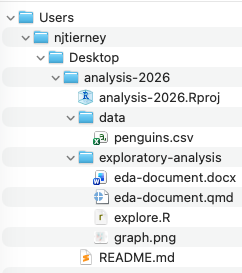
\includegraphics[keepaspectratio]{figs/project-org-file-explorer.png}}

\emph{Example of file and folder structure}

Each level is a folder inside the one above it. To read that data file,
you might write:

\begin{Shaded}
\begin{Highlighting}[]
\NormalTok{penguins }\OtherTok{\textless{}{-}} \FunctionTok{read\_csv}\NormalTok{(}\StringTok{"/Users/njtierney/Desktop/analysis{-}2026/data/penguins.csv"}\NormalTok{)}
\end{Highlighting}
\end{Shaded}

So in the above, the ``path'' is
\texttt{"/Users/njtierney/Desktop/analysis-2026/data/penguins.csv"}.

You might also note that sometimes in your work, you don't write down
this full path - it is very long! You might do something like:

\begin{Shaded}
\begin{Highlighting}[]
\NormalTok{penguins }\OtherTok{\textless{}{-}} \FunctionTok{read\_csv}\NormalTok{(}\StringTok{"data/penguins.csv"}\NormalTok{)}
\end{Highlighting}
\end{Shaded}

And this brings us to an important concept - these are two kinds of
path:

\begin{itemize}
\tightlist
\item
  \textbf{absolute paths} starts from the root of your computer.
\item
  \textbf{relative paths} starts from wherever you currently are.
\end{itemize}

To continue our directions analogy:

\begin{itemize}
\tightlist
\item
  \textbf{absolute paths} - the full driving directions to take you from
  Hobart to Cradle Mountain
\item
  \textbf{relative paths} - the directions from where you are (which
  might be just down the road!) to Cradle Mountain.
\end{itemize}

So, the code below is using an absolute path:

\begin{Shaded}
\begin{Highlighting}[]
\NormalTok{penguins }\OtherTok{\textless{}{-}} \FunctionTok{read\_csv}\NormalTok{(}\StringTok{"/Users/njtierney/Desktop/analysis{-}2026/data/penguins.csv"}\NormalTok{)}
\end{Highlighting}
\end{Shaded}

The code below is using a relative path:

\begin{Shaded}
\begin{Highlighting}[]
\NormalTok{penguins }\OtherTok{\textless{}{-}} \FunctionTok{read\_csv}\NormalTok{(}\StringTok{"data/penguins.csv"}\NormalTok{)}
\end{Highlighting}
\end{Shaded}

Of the two, the relative path might look nice, because it is shorter.
And that's sort of true.

But the absolute path will work from anywhere on your machine. Every
time. Now.

But will it work on your colleagues machine? On your machine in two
weeks, next month, next year?

My absolute path will not work on your machine, because your computer
(almost certainly) doesn't have a \texttt{/Users/njtierney/} folder. It
won't work on your own machine after you reorganise your folders when
you spring clean. It won't work on the cloud.

\begin{tcolorbox}[enhanced jigsaw, arc=.35mm, bottomrule=.15mm, bottomtitle=1mm, breakable, colback=white, colbacktitle=quarto-callout-note-color!10!white, colframe=quarto-callout-note-color-frame, coltitle=black, left=2mm, leftrule=.75mm, opacityback=0, opacitybacktitle=0.6, rightrule=.15mm, title=\textcolor{quarto-callout-note-color}{\faInfo}\hspace{0.5em}{Your Turn}, titlerule=0mm, toprule=.15mm, toptitle=1mm]

\begin{enumerate}
\def\labelenumi{\arabic{enumi}.}
\tightlist
\item
  Imagine you see the path
  \texttt{/Users/miles/etc1010/week1/data/health.csv}. What are the
  folders above the file \texttt{health.csv}?
\item
  Run \texttt{getwd()}. Where are you?
\item
  Look at your most recent analysis script. Find every file path in it.
  How many are absolute?
\end{enumerate}

\end{tcolorbox}

A common answer to this is that people will often use relative paths,
along with a function \texttt{setwd()}:

\begin{Shaded}
\begin{Highlighting}[]
\FunctionTok{setwd}\NormalTok{(}\StringTok{"/Users/njtierney/Desktop/analysis{-}2026"}\NormalTok{)}
\NormalTok{penguins }\OtherTok{\textless{}{-}} \FunctionTok{read\_csv}\NormalTok{(}\StringTok{"data/penguins.csv"}\NormalTok{)}
\end{Highlighting}
\end{Shaded}

Let's talk about why this is \textbf{not a good idea}.

\section{\texorpdfstring{What does \texttt{setwd()}
do?}{What does setwd() do?}}\label{what-does-setwd-do}

Sometimes the first line of a script looks like this:

\begin{Shaded}
\begin{Highlighting}[]
\FunctionTok{setwd}\NormalTok{(}\StringTok{"/Users/njtierney/Desktop/analysis{-}2026"}\NormalTok{)}
\end{Highlighting}
\end{Shaded}

This says:

\begin{quote}
Set my working directory to this specific directory, ``analysis-2026'',
which is in the folders, Users/njtierney/Desktop.
\end{quote}

It means you can then read data using the \textbf{relative paths} we
discussed above:

\begin{Shaded}
\begin{Highlighting}[]
\NormalTok{penguins }\OtherTok{\textless{}{-}} \FunctionTok{read\_csv}\NormalTok{(}\StringTok{"data/penguins.csv"}\NormalTok{)}
\end{Highlighting}
\end{Shaded}

instead of using the \textbf{absolute path}:

\begin{Shaded}
\begin{Highlighting}[]
\NormalTok{penguins }\OtherTok{\textless{}{-}} \FunctionTok{read\_csv}\NormalTok{(}\StringTok{"/Users/njtierney/Desktop/analysis{-}2026/data/penguins.csv"}\NormalTok{)}
\end{Highlighting}
\end{Shaded}

So it does have the effect of \textbf{making the file paths work in your
file}.

But, it is still a problem, because using \texttt{setwd()} like this
creates the same problem you had when you used the \textbf{absolute
path}:

\begin{itemize}
\tightlist
\item
  0\% chance of working on someone else's machine --- \textbf{and this
  could include you, in six months}.
\item
  Means your file is not self-contained or portable. What happens if
  this folder moves to \texttt{/Downloads}, or onto another machine?
\end{itemize}

I used to send files to people like this, and you might have come across
this yourself - where an R file comes to you and your colleague says:

\begin{quote}
Yup, all you need to do is \textbf{change the
\texttt{setwd("/Users/njtierney/Desktop/analysis-2026")} to point at
where you are, then run it}
\end{quote}

So, to get it working, you have to hand-edit the file path for every
machine it lands on.

This is painful. And when you do it all the time, it gets old, fast.
There is a better way!

\begin{figure}[ht]

{\centering 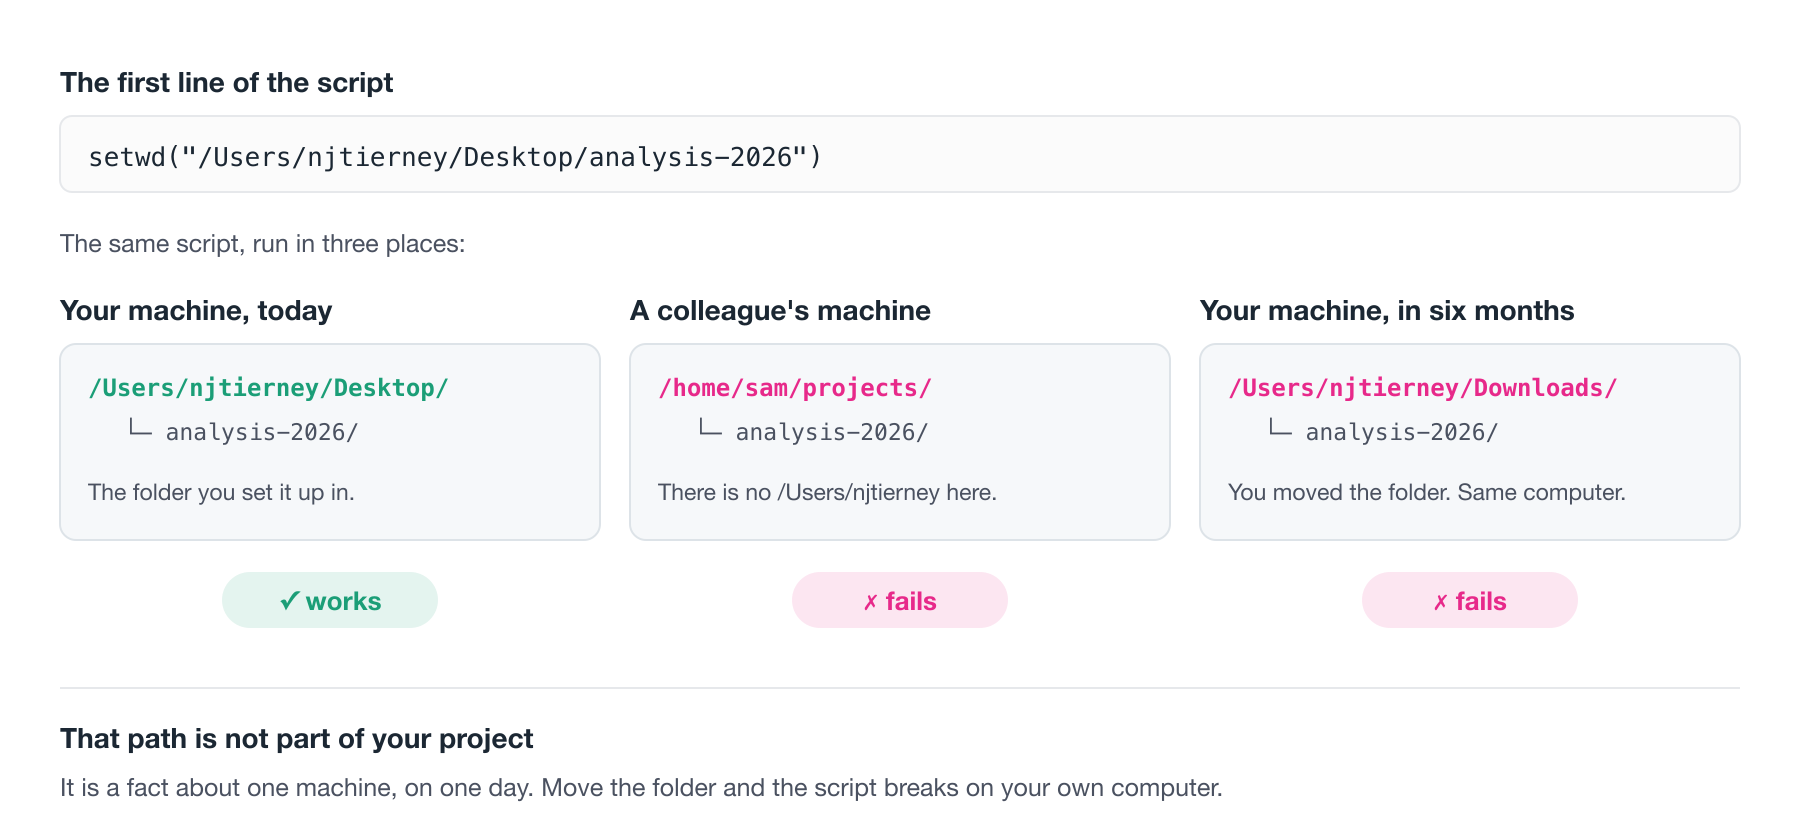
\includegraphics[width=1\linewidth,height=\textheight,keepaspectratio,alt={A script whose first line is setwd to /Users/njtierney/Desktop/analysis-2026, shown running in three places. On your own machine today the project really is under /Users/njtierney/Desktop, and the script works. On a colleague\textquotesingle s machine the project sits under /home/sam/projects, and the script fails. On your own machine six months later, the folder has moved to /Users/njtierney/Downloads, and the script fails again. That path is a fact about one machine on one day, not part of the project.}]{figs/setwd-one-machine.png}

}

\caption{The path inside \texttt{setwd()} names a folder that only one
machine has, and will not work in future places.}

\end{figure}%

This is the heart of the famous line from Jenny Bryan, from her
brilliant article,
\href{https://tidyverse.org/blog/2017/12/workflow-vs-script/}{``Project-oriented
workflow''}- you should read it:

\begin{quote}
If the first line of your R script is

\begin{verbatim}
setwd("C:\Users\jenny\path\that\only\I\have")
\end{verbatim}

I will come into your office and SET YOUR COMPUTER ON FIRE 🔥.
\end{quote}

\section{Is there an answer to the
madness?}\label{is-there-an-answer-to-the-madness}

Yes.

When you start on a new idea, a new project, a new paper --- anything
new --- it should start its life as a \textbf{project}. In RStudio that
is an \texttt{.Rproj} file; in Positron it is a \textbf{workspace
folder}.

A project keeps related work together in the same place. They also do
the following:

\begin{itemize}
\tightlist
\item
  Keep all your files together.
\item
  Set the working directory to the project directory.
\item
  Start a new session of R.
\item
  Restore previously edited files into your editor tabs.
\item
  Restore other editor settings.
\item
  Let you have several projects open at once.
\end{itemize}

This helps keep you sane, because:

\begin{itemize}
\tightlist
\item
  Your projects are each independent.
\item
  You can work on different projects at the same time.
\item
  Objects and functions you create in one project won't affect another.
\item
  You can refer to your data in a consistent way.
\end{itemize}

And finally, the big one:

\textbf{Projects resolve file path problems}, because they automatically
set the working directory to the location of the project.

This means you get two habits from this:

\begin{enumerate}
\def\labelenumi{\arabic{enumi}.}
\tightlist
\item
  \textbf{One project, one folder, one \texttt{.Rproj} file.} Open the
  project by double-clicking the \texttt{.Rproj} file, not by opening R
  and navigating around.
\item
  \textbf{Use relative paths only.} You never call \texttt{setwd()}
  again.
\end{enumerate}

\begin{tcolorbox}[enhanced jigsaw, arc=.35mm, bottomrule=.15mm, bottomtitle=1mm, breakable, colback=white, colbacktitle=quarto-callout-caution-color!10!white, colframe=quarto-callout-caution-color-frame, coltitle=black, left=2mm, leftrule=.75mm, opacityback=0, opacitybacktitle=0.6, rightrule=.15mm, title=\textcolor{quarto-callout-caution-color}{\faFire}\hspace{0.5em}{Aside: creating a project}, titlerule=0mm, toprule=.15mm, toptitle=1mm]

\section{RStudio}

Either use the button in the top right corner, or go:

File → New Project → New Directory → New Project → name your project →
Create Project

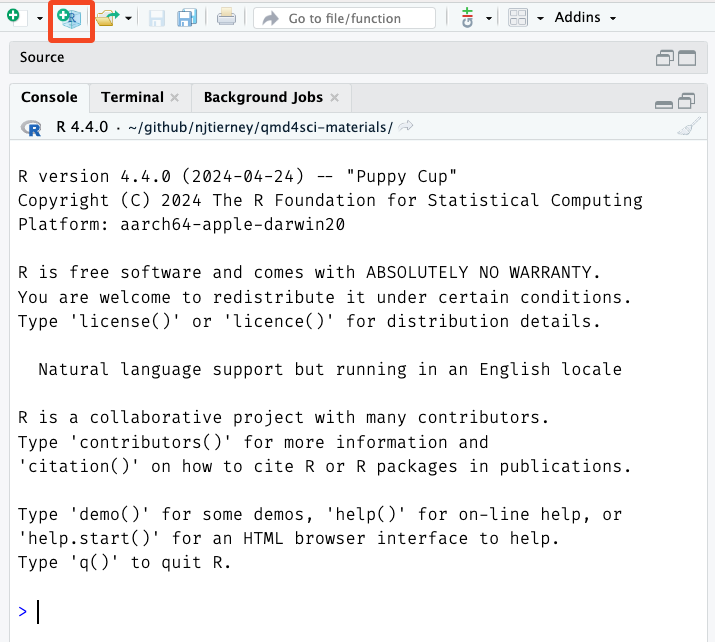
\includegraphics[width=0.7\linewidth,height=\textheight,keepaspectratio]{figs/rstudio-create-proj-1.png}

\emph{Starting a new project in RStudio.}

Then choose \textbf{New Directory} if this is a new folder. If you
already have a folder you want to turn into a project, choose
\textbf{Existing Directory} instead.

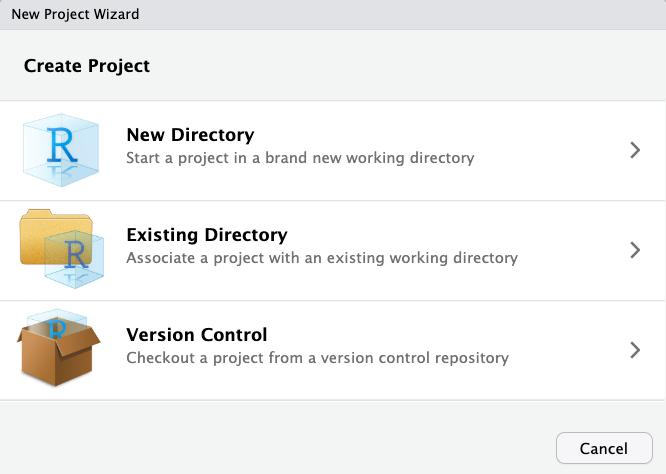
\includegraphics[width=0.7\linewidth,height=\textheight,keepaspectratio]{figs/rstudio-create-proj-2.png}

\emph{Choosing a new or existing directory.}

Then \textbf{New Project}.

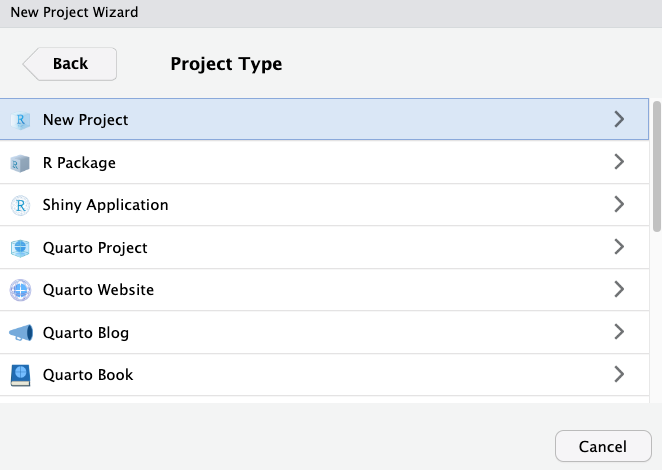
\includegraphics[width=0.7\linewidth,height=\textheight,keepaspectratio]{figs/rstudio-create-proj-3.png}

\emph{Choosing the project type.}

Then name it, and click \textbf{Create Project}.

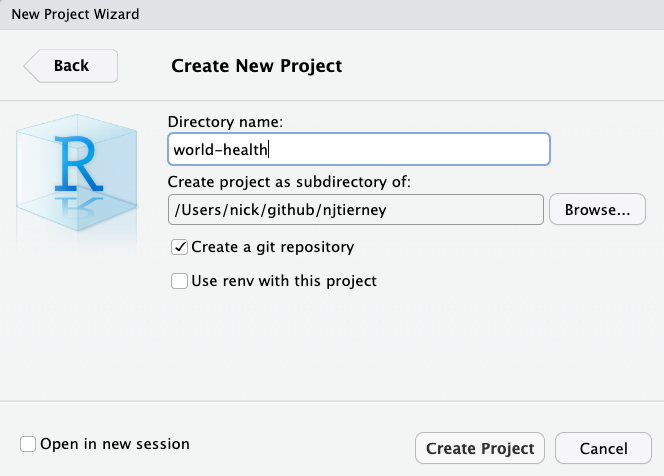
\includegraphics[width=0.7\linewidth,height=\textheight,keepaspectratio]{figs/rstudio-create-proj-4.png}

\emph{Naming the project.}

\section{Positron}

Positron doesn't use .Rproj files - that is an RStudio specific file.

The posit team talk about this in their docs:
\href{https://positron.posit.co/migrate-rstudio-rproj.html}{``The R Proj
File''}.

The gist of this is that Positron does not have Rproj files - you
essentially just open a folder and Positron will treat it as a
``workspace''.

You can open a folder as a workspace: File -\textgreater{} Open Folder.

If you also want the project to work in RStudio, add an \texttt{.Rproj}
file:

\begin{Shaded}
\begin{Highlighting}[]
\NormalTok{usethis}\SpecialCharTok{::}\FunctionTok{use\_rstudio}\NormalTok{()}
\end{Highlighting}
\end{Shaded}

Either way, it is worth spending a couple of minutes on the name. Even a
few minutes can make a difference. You want to:

\begin{itemize}
\tightlist
\item
  Keep it short.
\item
  Use no spaces.
\item
  Combine words.
\end{itemize}

For example, I had a project looking at bat calls, so I called it
\texttt{screech}, because bats make a screech-y noise. If you are doing
global health analysis, maybe it is \texttt{world-health}.

\end{tcolorbox}

\section{The \{here\} package}\label{the-here-package}

Although projects resolve most file path problems, in some cases you
might have many nested folders. To navigate them reliably you can use
the \href{https://here.r-lib.org/}{\{here\}} package, which builds the
full path from the project root, compactly.

\begin{Shaded}
\begin{Highlighting}[]
\NormalTok{here}\SpecialCharTok{::}\FunctionTok{here}\NormalTok{(}\StringTok{"data"}\NormalTok{)}
\CommentTok{\#\textgreater{} [1] "/Users/njtierney/github/njtierney/analysis{-}2026/data"}
\end{Highlighting}
\end{Shaded}

and

\begin{Shaded}
\begin{Highlighting}[]
\NormalTok{here}\SpecialCharTok{::}\FunctionTok{here}\NormalTok{(}\StringTok{"data"}\NormalTok{, }\StringTok{"penguins.csv"}\NormalTok{)}
\CommentTok{\#\textgreater{} [1] "/Users/njtierney/github/njtierney/analysis{-}2026/data/penguins.csv"}
\end{Highlighting}
\end{Shaded}

Note that these absolute paths will be different on my computer compared
to yours --- which is exactly the point.

You can read that \texttt{here} code as:

\begin{quote}
In the folder \texttt{data}, there is a file called
\texttt{penguins.csv}. Can you please give me the full path to that
file?
\end{quote}

This is handy for a few reasons:

\begin{enumerate}
\def\labelenumi{\arabic{enumi}.}
\tightlist
\item
  It makes things \emph{completely} portable.
\item
  Quarto documents have their own way of looking for files, and this
  eliminates a whole class of file path pain.
\item
  If you decide not to use projects, you still have code that works on
  \emph{any} machine.
\end{enumerate}

So in practice:

\begin{Shaded}
\begin{Highlighting}[]
\FunctionTok{library}\NormalTok{(here)}
\NormalTok{penguins }\OtherTok{\textless{}{-}} \FunctionTok{read\_csv}\NormalTok{(}\FunctionTok{here}\NormalTok{(}\StringTok{"data"}\NormalTok{, }\StringTok{"penguins.csv"}\NormalTok{))}
\end{Highlighting}
\end{Shaded}

works whether the code is called from the top of the project, from
inside \texttt{analysis/}, or from a Quarto document being rendered in a
subfolder --- all places where a plain relative path can quietly mean
something different.

\begin{tcolorbox}[enhanced jigsaw, arc=.35mm, bottomrule=.15mm, bottomtitle=1mm, breakable, colback=white, colbacktitle=quarto-callout-note-color!10!white, colframe=quarto-callout-note-color-frame, coltitle=black, left=2mm, leftrule=.75mm, opacityback=0, opacitybacktitle=0.6, rightrule=.15mm, title=\textcolor{quarto-callout-note-color}{\faInfo}\hspace{0.5em}{Your Turn}, titlerule=0mm, toprule=.15mm, toptitle=1mm]

\begin{enumerate}
\def\labelenumi{\arabic{enumi}.}
\tightlist
\item
  Open a project of your own, and run \texttt{here::here()}. Is it where
  you expected?
\item
  Take one absolute path from your most recent script and rewrite it
  with \texttt{here()}.
\item
  What would have to be true about your working directory for the old
  version to work?
\end{enumerate}

\end{tcolorbox}

\begin{tcolorbox}[enhanced jigsaw, arc=.35mm, bottomrule=.15mm, bottomtitle=1mm, breakable, colback=white, colbacktitle=quarto-callout-note-color!10!white, colframe=quarto-callout-note-color-frame, coltitle=black, left=2mm, leftrule=.75mm, opacityback=0, opacitybacktitle=0.6, rightrule=.15mm, title=\textcolor{quarto-callout-note-color}{\faInfo}\hspace{0.5em}{Your Turn}, titlerule=0mm, toprule=.15mm, toptitle=1mm]

When you start a \textbf{new} project:

\begin{itemize}
\tightlist
\item
  What is your normal workflow?
\item
  What helps you, what hinders you?
\item
  What do you think you should do?
\end{itemize}

When you come back to an \textbf{old} project:

\begin{itemize}
\tightlist
\item
  What has made it easier to work on it?
\item
  What makes it difficult?
\item
  Anything you wish you did?
\end{itemize}

There are no wrong answers! I want to have a discussion, and learn what
wins, what makes it hard, what makes it OK.

\end{tcolorbox}

\section{Why organise your project?}\label{why-organise-your-project}

When you are working on a project, you are almost certainly going to be
returning to it, at some point. When you do, you might look at the code,
and wonder:

\begin{quote}
Who wrote this, and are they insane?
\end{quote}

And then you realise that indeed, \textbf{it was you} that wrote this.

I think it is worthwhile internalising this saying:

\begin{quote}
You are always collaborating with your future self.\footnote{I swear I
  heard ot from someone else, but I cannot find the source}
\end{quote}

You want to have notes that keep you organised, and help you return to
work smoothly. I think the ``Who what when where why how'' of story
telling can be really useful here:

\begin{itemize}
\tightlist
\item
  \textbf{Who} did it: Was it just you? Were there many people?
\item
  \textbf{What} you did: what was run
\item
  \textbf{When} you did it: Last year, last month?
\item
  \textbf{Where} you did it: on your computer? the cloud?
\item
  \textbf{Why} you did it: what was the goal
\item
  \textbf{How} you did it: What was the order you ran things? Which file
  should I look at first?
\end{itemize}

If you can't answer these questions about a project, how much harder
would it be for you to return to it?

It is like making sure your house is tidy, and the dishes are done. It
is \emph{technically} optional, sure. But, it does make your life easier
when things are tidy, and always in the same spot.

I like to think of this as some self-care for your future self.

What I am getting at here is:

\begin{quote}
\textbf{A project that is organised is a project that's more likely to
re-run.}
\end{quote}

A well organised project does not guarantee reproducibility. But, if you
can't tell me which script to run first, then we cannot reproduce an
analysis.

The point is not to tidy your project just so it is tidy. The point is
having a tidy project that is well organised makes it easier to check,
run later, and understand.

Note: I think I'd like to very quickly just give people a win here and
show them that this part of the lesson is just: write a README, folks.
And then some additional motivation

Note: I need a preamble link into the next section, or consider moving
these sections around.

\section{Pitfalls of organisation}\label{pitfalls-of-organisation}

There are so many ways to organise a project. And there is no one
correct. And organising a project well is hard. While there isn't a
\textbf{right} way, there are definitely \textbf{better} and
\textbf{worse} ways. Circling back to the start of the lesson, one of
the takeaways from today I want you to remember is:

\begin{quote}
Your project might not be perfectly organised, but it should be possible
for someone to understand how it is structured, and what to run first.
\end{quote}

There are a few patterns that I think appear in projects. I am guilty of
all of these, so know that I am not judging you if these are how you
work now. What I am saying is that it is OK, and that there are some
ways you can improve.

I have put most of these patterns together into one repository, which
you can see at:

https://github.com/njtierney/rbp-materials

\subsection{Everything in one folder}\label{everything-in-one-folder}

\begin{verbatim}
01-everything-in-one-folder/
├── Rplot.png
├── Screen Shot 2026-03-14 at 10.23.45 am.png
├── Untitled1.R
├── analysis.R
├── figure1.png
├── notes.txt
├── penguins.csv
├── plot_stuff.R
├── report draft.docx
└── results.csv
\end{verbatim}

Notice that the R scripts, the data, the figures, a Word document, a
screenshot, and \texttt{Untitled1.R}, are all \emph{flat} - they are in
the same folder. This works until there are more than about fifteen
files, at which point finding anything becomes a search problem.

I think about this as like a grocery list: If my shopping list is only 5
items long, it might not impact me when I go to the shops:

\begin{itemize}
\tightlist
\item
  Milk
\item
  Yoghurt
\item
  Muesli
\item
  Bananas
\item
  Muesli bars
\end{itemize}

But if I'm buying a bunch of food for the week, some meal prep, and a
few other bits and pieces, if I don't order the shopping list, and group
the similar parts together, I am creating work for myself.

\section{Unordered}

\begin{itemize}
\tightlist
\item
  Milk
\item
  Onion powder
\item
  Red capsicum
\item
  Yoghurt
\item
  Muesli
\item
  Bananas
\item
  Muesli bars
\item
  Tomato paste
\item
  Ginger
\item
  Coriander
\item
  Garlic
\item
  Lemongrass
\item
  Coconut milk
\item
  Chicken thighs
\item
  Limes
\item
  Eggplants
\item
  Snow peas
\item
  Thai basil
\item
  500g beef mince
\item
  Basmati rice
\end{itemize}

\section{Ordered}

\begin{itemize}
\tightlist
\item
  \textbf{Produce}

  \begin{itemize}
  \tightlist
  \item
    Bananas
  \item
    Ginger
  \item
    Garlic
  \item
    Lemongrass
  \item
    Limes
  \item
    Thai basil
  \item
    Coriander
  \item
    Eggplants
  \item
    Red capsicum
  \item
    Snow peas
  \end{itemize}
\item
  \textbf{Dairy}

  \begin{itemize}
  \tightlist
  \item
    Milk
  \item
    Yoghurt
  \end{itemize}
\item
  \textbf{Meat}

  \begin{itemize}
  \tightlist
  \item
    Chicken thighs
  \item
    500g beef mince
  \end{itemize}
\item
  \textbf{Pantry}

  \begin{itemize}
  \tightlist
  \item
    Muesli
  \item
    Muesli bars
  \item
    Basmati rice
  \item
    Coconut milk
  \item
    Tomato paste
  \item
    Onion powder
  \end{itemize}
\end{itemize}

\begin{itemize}
\tightlist
\item
  The problem: Flat directory structure can make it hard to group things
  to understand how they are related.
\item
  The (partial) solution: Put similar things into folders (directories)
  that give them structure.
\end{itemize}

\subsection{No clear entry point}\label{no-clear-entry-point}

\begin{verbatim}
02-no-clear-entry-point/
├── analysis.R
├── clean.R
├── data.csv
├── do_it.R
├── final.R
├── helpers.R
├── main.R
├── model.R
├── plots.R
├── run.R
├── script.R
└── tests.R
\end{verbatim}

There are eleven \texttt{.R} files and no way to tell which one runs
first. If the only way to know the order they are run in, is only in
your head, the project is not reproducible. It is a performance that
only you can give.

\begin{itemize}
\tightlist
\item
  The problem: When task order is required, but it is not written down,
  you cannot reproduce the task.
\item
  The outcome: Encode the task order in another file, such as
  ``make-project.R'', and/or put the files in order.
\end{itemize}

\section{File names encode history, not
content}\label{file-names-encode-history-not-content}

\begin{verbatim}
04-names-encode-history/
├── analysis.R
├── analysis2.R
├── analysis_final.R
├── analysis_final_USE_THIS_ONE.R
├── analysis_final_USE_THIS_ONE_v2 (nick edits).R
├── analysis_final_USE_THIS_ONE_v2.R
├── analysis_final_v2.R
└── penguins.csv
\end{verbatim}

The \emph{names} of these files tell a story: the analysis progressed,
things changed, and there were concerns about knowing which version
worked, and being able to go back and change things. You can think of
this as using ``track changes'' in a word document. This is a kind of
version control. But naming the files in order to track versions creates
problems, and it is better solved with specific version control
software, such as git. I cover this in another course,
\href{https://gentle-git.njtierney.com/}{``Introduction to git and
github''}.

\begin{itemize}
\tightlist
\item
  The problem: There are multiples of the same file with names that tell
  you their version, rather than their task.
\item
  The solution: Name the files for what they do, not when you made them.
  Use a version control system like \href{}{git}
\end{itemize}

\section{Editing raw data in place}\label{editing-raw-data-in-place}

You might have some data provided for analysis and there might be
instructions to go through by hand to fix typos, or add new data. You
should not make hand edits to the file, as this changes the history and
increases the chances of a non-repeatable change. You can make a
critical error by accidentally hitting the wrong key. From experience,
having accidentally sorted a single column in an excel sheet and not
realising this, I essentially turned a meaningful data source into
random noise.

\begin{itemize}
\tightlist
\item
  The problem: Hand editing raw data
\item
  The solution: raw data should be read-only, and changes that happen to
  it happen with code, and are saved to separate outputs.
\end{itemize}

\section{Outputs mixed in with
inputs}\label{outputs-mixed-in-with-inputs}

\begin{verbatim}
03-outputs-mixed-with-inputs/
├── 01-clean.R
├── 02-model.R
├── cleaned_data.csv
├── fig-mass-flipper.png
├── fig-species.png
├── model_fit.rds
├── penguins.csv
└── raw survey data.xlsx
\end{verbatim}

In this case, figures, model outputs, and cleaned data sit in the same
folder as your raw data and scripts. This mean that you cannot tell at a
glance what is necessary for your analysis, and what is produced as
output by your analysis. If you cannot tell what is input, and what is
output, it means you don't have a clear sense of how to reproduce files,
or where edits can be safely made. A good test: \emph{could I delete
this folder entirely and regenerate it by running my code?} If yes, it
is an output, and it should live somewhere that says so.

\begin{itemize}
\tightlist
\item
  The problem: Not knowing what is inputs vs outputs impacts
  reproducibility.
\item
  The solution: Clearly label inputs and outputs - potentially put your
  outputs in an ``outputs'' folder. Or have a file that describes the
  inputs and outputs, such as a README, or an analysis script.
\end{itemize}

\begin{tcolorbox}[enhanced jigsaw, arc=.35mm, bottomrule=.15mm, bottomtitle=1mm, breakable, colback=white, colbacktitle=quarto-callout-note-color!10!white, colframe=quarto-callout-note-color-frame, coltitle=black, left=2mm, leftrule=.75mm, opacityback=0, opacitybacktitle=0.6, rightrule=.15mm, title=\textcolor{quarto-callout-note-color}{\faInfo}\hspace{0.5em}{Your Turn}, titlerule=0mm, toprule=.15mm, toptitle=1mm]

Open a project you worked on more than six months ago.

\begin{enumerate}
\def\labelenumi{\arabic{enumi}.}
\tightlist
\item
  Can you tell, within thirty seconds, which script to run first?
\item
  Which files could you delete and regenerate from code?
\item
  Which files could you \emph{not} regenerate? Those are the ones that
  actually matter --- are they backed up?
\end{enumerate}

\end{tcolorbox}

\section{Common project structures}\label{common-project-structures}

There is no single correct structure, but there is a common shape that
most working structures converge on:

\begin{figure}[ht]

{\centering 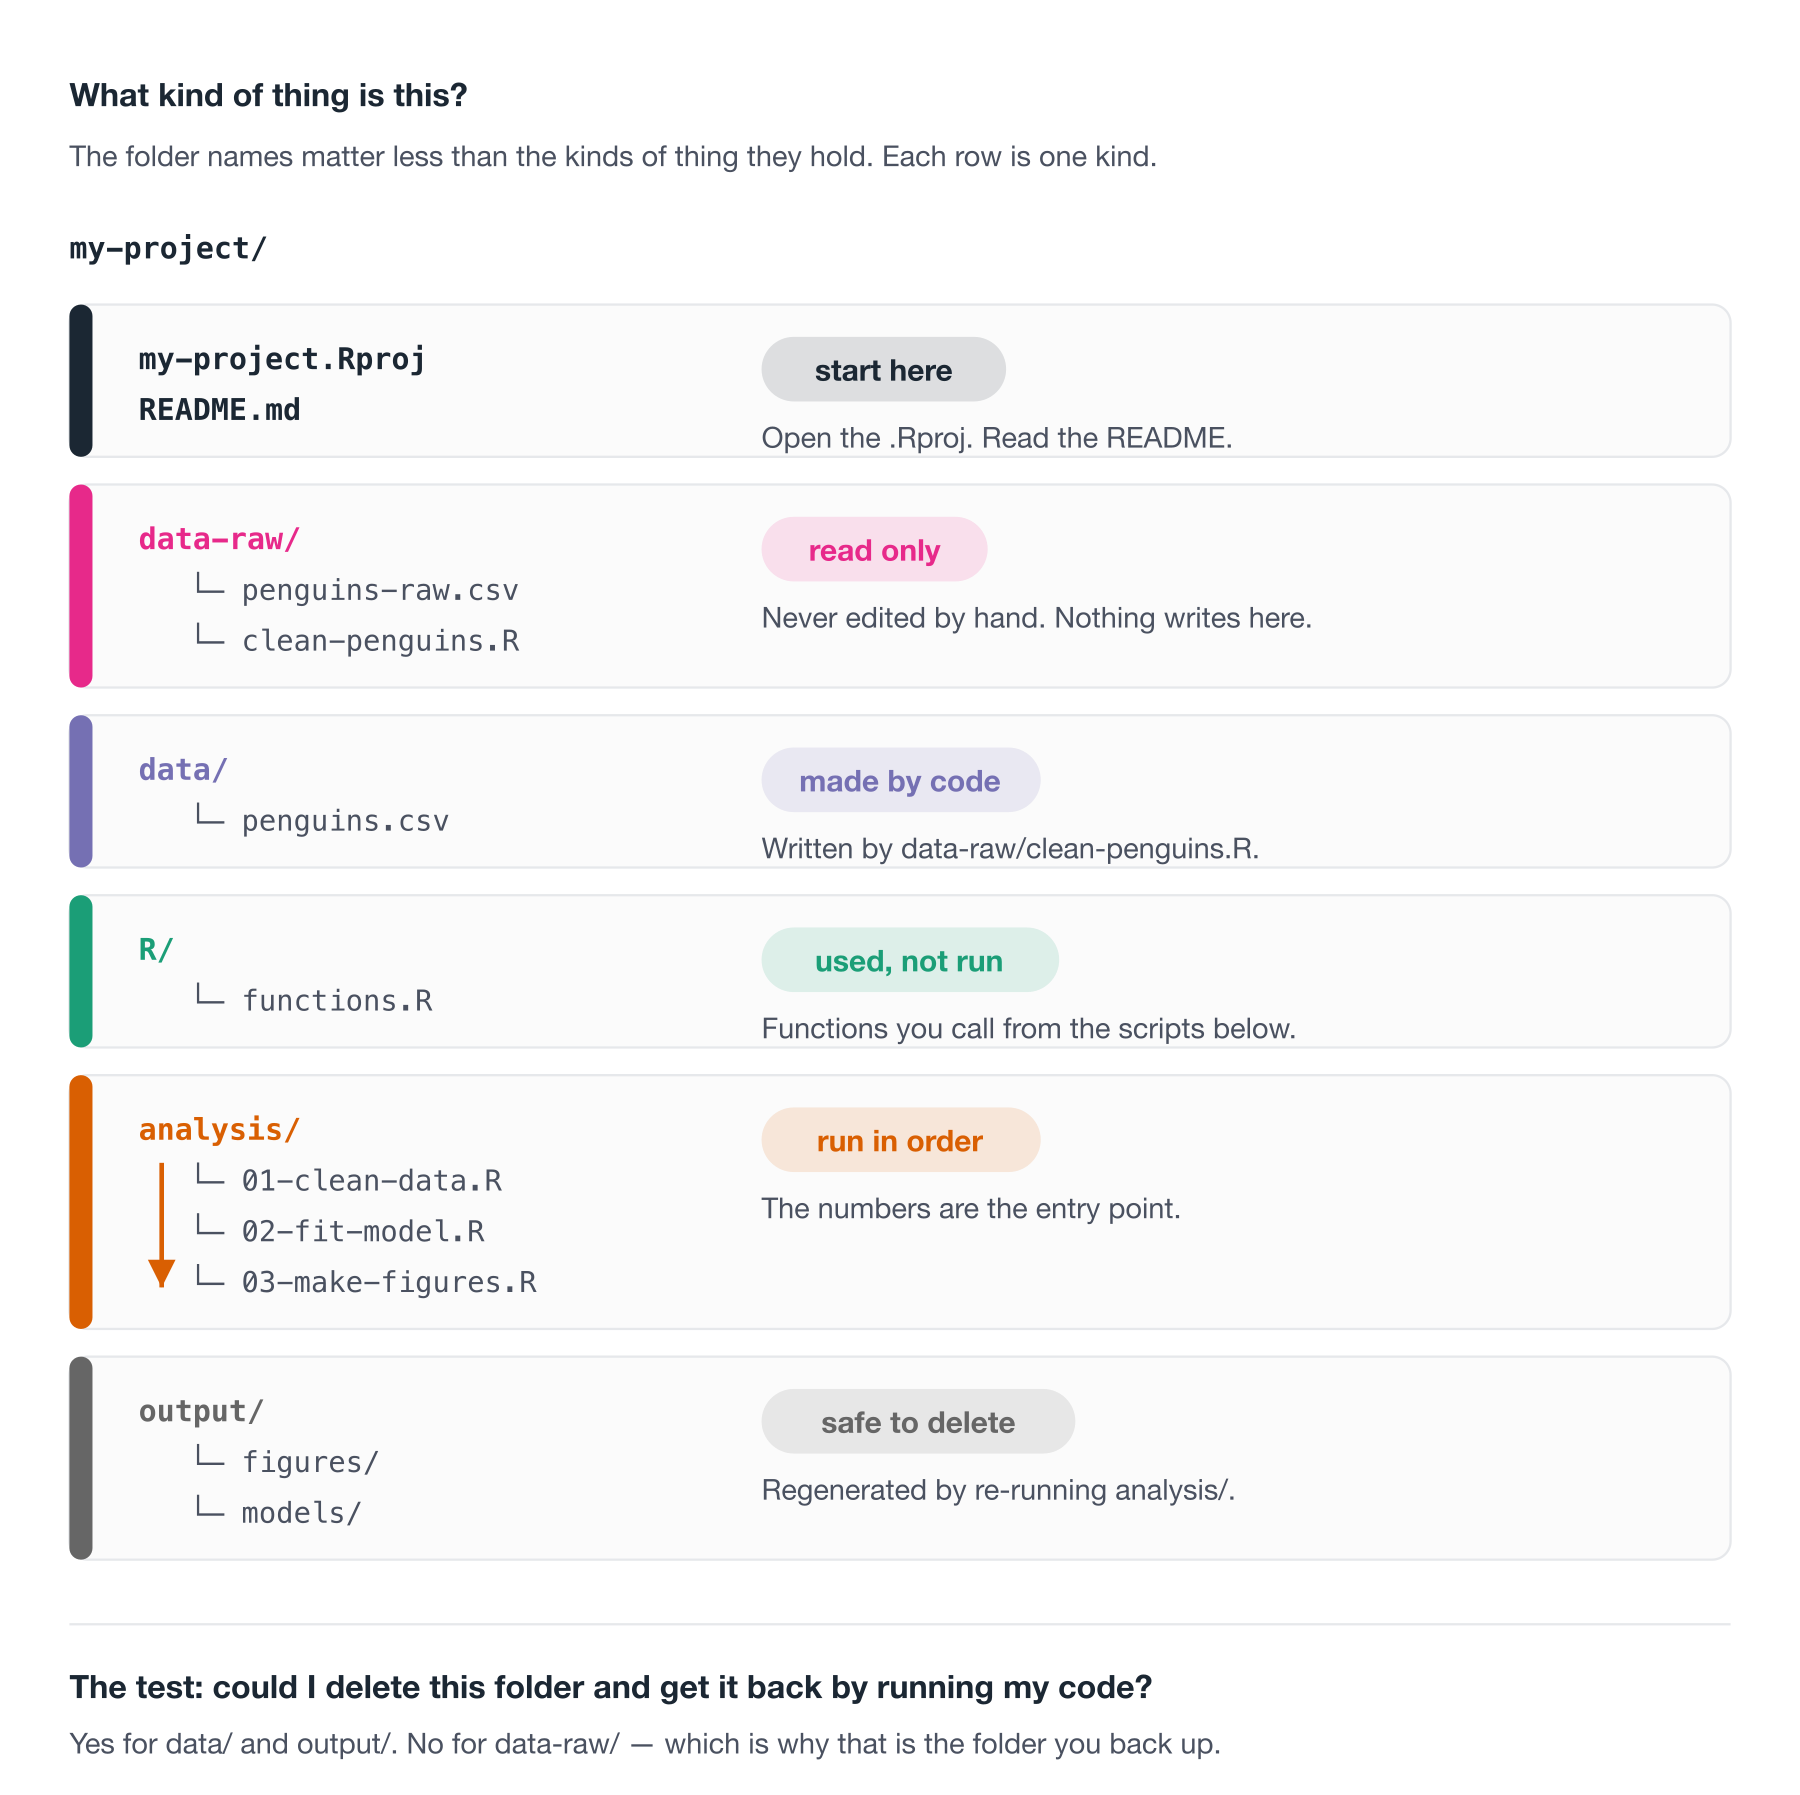
\includegraphics[width=1\linewidth,height=\textheight,keepaspectratio,alt={A project folder called my-project, drawn as six rows, one for each kind of thing it holds. Row one: my-project.Rproj and README.md, labelled start here --- open the .Rproj, read the README. Row two: data-raw/ containing penguins-raw.csv and clean-penguins.R, labelled read only --- never edited by hand, nothing writes here. Row three: data/ containing penguins.csv, labelled made by code --- written by data-raw/clean-penguins.R. Row four: R/ containing functions.R, labelled used, not run --- functions you call from the scripts below. Row five: analysis/ containing 01-clean-data.R, 02-fit-model.R and 03-make-figures.R, labelled run in order, with an arrow running down the three numbered scripts. Row six: output/ containing figures/ and models/, labelled safe to delete --- regenerated by re-running analysis/. Underneath, the test: could I delete this folder and get it back by running my code? Yes for data/ and output/, no for data-raw/, which is why that is the folder you back up.}]{figs/project-structure-kinds.png}

}

\caption{The same structure, grouped by what each thing \emph{is} rather
than what it is called. Raw data is read only, code in \texttt{R/} gets
used, scripts in \texttt{analysis/} get run in order, and everything in
\texttt{output/} can be deleted and regenerated.}

\end{figure}%

The parts worth noticing:

\begin{itemize}
\tightlist
\item
  \textbf{\texttt{data-raw/} holds the raw data, exactly as you received
  it}, along with the script that cleans it. Raw data is read-only, so
  nothing ever writes here, and you never edit it by hand. Keeping the
  cleaning script next to the raw data means the two never drift apart.
\item
  \textbf{\texttt{data/} holds the analysis-ready data} that the
  cleaning script produces. This is the version your analysis actually
  reads.
\item
  \textbf{\texttt{R/} holds functions.} Code that gets \emph{used}, not
  code that gets \emph{run}. We will spend a whole lesson on this.
\item
  \textbf{\texttt{analysis/} holds scripts that get run}, in order. The
  numbering is doing real work: it tells your future self the entry
  point without needing a README.
\item
  \textbf{\texttt{output/} holds things you can delete.} Anything in
  here can be regenerated by re-running the analysis.
\end{itemize}

If your project is small, collapse this. Three files in a flat folder
with a README is a perfectly good project structure. The point is not to
have folders. It is to have \emph{a place where each kind of thing
goes}, and to be consistent about it.

\begin{tcolorbox}[enhanced jigsaw, arc=.35mm, bottomrule=.15mm, bottomtitle=1mm, breakable, colback=white, colbacktitle=quarto-callout-tip-color!10!white, colframe=quarto-callout-tip-color-frame, coltitle=black, left=2mm, leftrule=.75mm, opacityback=0, opacitybacktitle=0.6, rightrule=.15mm, title=\textcolor{quarto-callout-tip-color}{\faLightbulb}\hspace{0.5em}{The same structure as text, if you want to copy it}, titlerule=0mm, toprule=.15mm, toptitle=1mm]

\begin{verbatim}
my-project/
|-- my-project.Rproj
|-- README.md
|-- data-raw/
|   |-- penguins-raw.csv
|   `-- clean-penguins.R
|-- data/
|   `-- penguins.csv
|-- R/
|   `-- functions.R
|-- analysis/
|   |-- 01-clean-data.R
|   |-- 02-fit-model.R
|   `-- 03-make-figures.R
`-- output/
    |-- figures/
    `-- models/
\end{verbatim}

\end{tcolorbox}

\subsection{Naming the files
themselves}\label{naming-the-files-themselves}

Naming is hard. We will come back to this throughout the course.

This structure tells you \textbf{where} things go, but it does not tell
you what to \textbf{name} them.

The \href{https://style.tidyverse.org/files.html}{files chapter of the
Tidyverse style guide} is short, and it is worth your time reading. I
also really enjoy Jenny Bryan's talk,
\href{https://github.com/jennybc/how-to-name-files}{``How to name files
like a normie''}:

Some especially good pieces of advice:

\begin{itemize}
\tightlist
\item
  \textbf{Machine readable.} No spaces, no punctuation beyond \texttt{-}
  and \texttt{\_}, and stick to one case. \texttt{01-clean-data.R}, not
  \texttt{01\ Clean\ Data\ (final).R}.
\item
  \textbf{Human readable.} The name should say what the file does.
  \texttt{clean-penguins.R} tells you something. \texttt{script2.R} does
  not.
\item
  \textbf{Sorts sensibly.} Numbers at the front, zero padded, so
  \texttt{01}, \texttt{02}, \texttt{10} stay in order. Dates as
  \texttt{YYYY-MM-DD}, which sorts correctly for free.
\end{itemize}

That last one is the sneaky one. If your file names sort properly, your
file explorer does your project organisation for you, and you get the
running order without needing a README.

You still need the README, of course.

\begin{tcolorbox}[enhanced jigsaw, arc=.35mm, bottomrule=.15mm, bottomtitle=1mm, breakable, colback=white, colbacktitle=quarto-callout-note-color!10!white, colframe=quarto-callout-note-color-frame, coltitle=black, left=2mm, leftrule=.75mm, opacityback=0, opacitybacktitle=0.6, rightrule=.15mm, title=\textcolor{quarto-callout-note-color}{\faInfo}\hspace{0.5em}{Your Turn}, titlerule=0mm, toprule=.15mm, toptitle=1mm]

Look at the file names in your most recent project.

\begin{enumerate}
\def\labelenumi{\arabic{enumi}.}
\tightlist
\item
  How many have spaces in them?
\item
  If you sorted them alphabetically, would the order mean anything?
\item
  Pick the worst named file and give it a better name.
\end{enumerate}

\end{tcolorbox}

\begin{tcolorbox}[enhanced jigsaw, arc=.35mm, bottomrule=.15mm, bottomtitle=1mm, breakable, colback=white, colbacktitle=quarto-callout-note-color!10!white, colframe=quarto-callout-note-color-frame, coltitle=black, left=2mm, leftrule=.75mm, opacityback=0, opacitybacktitle=0.6, rightrule=.15mm, title=\textcolor{quarto-callout-note-color}{\faInfo}\hspace{0.5em}{Your Turn}, titlerule=0mm, toprule=.15mm, toptitle=1mm]

Sketch the folder structure for a project you are working on right now.
Don't create it yet --- just write it out.

\begin{enumerate}
\def\labelenumi{\arabic{enumi}.}
\tightlist
\item
  Where does raw data go?
\item
  Where do the things you can regenerate go?
\item
  Where does someone start reading?
\end{enumerate}

\end{tcolorbox}

\section{``Good enough'' common sense principles of project
organisation}\label{good-enough-common-sense-principles-of-project-organisation}

I want to be clear that the goal here is \emph{good enough}, not
perfect. This phrasing comes from a paper I recommend to everyone,
\href{https://journals.plos.org/ploscompbiol/article?id=10.1371/journal.pcbi.1005510}{``Good
enough practices in scientific computing''} by Wilson and colleagues. It
is aimed at people who have real work to do and no appetite for
ceremony.

The principles I would hold you to:

\begin{enumerate}
\def\labelenumi{\arabic{enumi}.}
\tightlist
\item
  \textbf{Put each project in its own folder, with its own
  \texttt{.Rproj} file.}
\item
  \textbf{Treat raw data as read-only.} Never edit it by hand.
\item
  \textbf{Treat generated output as disposable.} If you can't delete it
  and get it back, it isn't really output.
\item
  \textbf{Use relative paths.} Never \texttt{setwd()}.
\item
  \textbf{Name files so a stranger can guess what they do.}
\item
  \textbf{Make the running order obvious}, with numbered scripts or a
  README.
\item
  \textbf{Write a README.}
\end{enumerate}

That is the whole list. If you do those seven things, you are organised
enough, and the remaining effort is better spent on the analysis itself.

One more principle, which is really about attitude:

\begin{quote}
Don't reorganise everything tonight.
\end{quote}

Apply this to your \emph{next} project. Retrofitting a large existing
project is a big job with a small payoff, and it is a very effective way
to talk yourself out of the whole idea. Start clean, once, and let the
habit build.

\begin{tcolorbox}[enhanced jigsaw, arc=.35mm, bottomrule=.15mm, bottomtitle=1mm, breakable, colback=white, colbacktitle=quarto-callout-note-color!10!white, colframe=quarto-callout-note-color-frame, coltitle=black, left=2mm, leftrule=.75mm, opacityback=0, opacitybacktitle=0.6, rightrule=.15mm, title=\textcolor{quarto-callout-note-color}{\faInfo}\hspace{0.5em}{Your Turn}, titlerule=0mm, toprule=.15mm, toptitle=1mm]

Go through the seven principles above and score your most recent project
out of seven.

Pick the single one that would have saved you the most time, and write
down what you would have to change to fix it.

\end{tcolorbox}

\section{Always have a README}\label{always-have-a-readme}

A README is a plain text file at the top of your project that answers
three questions:

\begin{enumerate}
\def\labelenumi{\arabic{enumi}.}
\tightlist
\item
  \textbf{What is this?}
\item
  \textbf{How do I run it?}
\item
  \textbf{Where does the data come from?}
\end{enumerate}

That's it. It does not need to be long. Mine are often ten lines. Here
is a complete, entirely adequate README:

\begin{Shaded}
\begin{Highlighting}[]
\FunctionTok{\# Penguin body mass analysis}

\NormalTok{Fits a model of penguin body mass against flipper length and species,}
\NormalTok{for the 2026 report to the department.}

\FunctionTok{\#\# How to run}

\NormalTok{Open }\InformationTok{\textasciigrave{}penguins.Rproj\textasciigrave{}}\NormalTok{, then run the scripts in }\InformationTok{\textasciigrave{}analysis/\textasciigrave{}}\NormalTok{ in order:}

\SpecialStringTok{1. }\InformationTok{\textasciigrave{}01{-}clean{-}data.R\textasciigrave{}}
\SpecialStringTok{2. }\InformationTok{\textasciigrave{}02{-}fit{-}model.R\textasciigrave{}}
\SpecialStringTok{3. }\InformationTok{\textasciigrave{}03{-}make{-}figures.R\textasciigrave{}}

\NormalTok{Figures are written to }\InformationTok{\textasciigrave{}output/figures/\textasciigrave{}}\NormalTok{.}

\FunctionTok{\#\# Data}

\InformationTok{\textasciigrave{}data/penguins.csv\textasciigrave{}}\NormalTok{ is from the \{palmerpenguins\} package, saved on}
\NormalTok{2026{-}03{-}14. Do not edit this file.}
\end{Highlighting}
\end{Shaded}

The reason I insist on this is that the README is the only part of your
project that explains \emph{intent}. Code tells you what happens. The
README tells you what you were trying to do, and that is the thing you
will have forgotten.

Write it first, if you can. A README written before the analysis is a
plan. A README written after the analysis is an archaeology report.

Two refinements worth knowing.

You can have \textbf{more than one README}. A short one inside
\texttt{data-raw/} explaining where those files came from is often the
most valuable file in the whole project.

And it's worth recording \textbf{when you obtained the data, and what
versions of software you used}, so that someone later, including you,
can reconstruct similar conditions.

\begin{tcolorbox}[enhanced jigsaw, arc=.35mm, bottomrule=.15mm, bottomtitle=1mm, breakable, colback=white, colbacktitle=quarto-callout-tip-color!10!white, colframe=quarto-callout-tip-color-frame, coltitle=black, left=2mm, leftrule=.75mm, opacityback=0, opacitybacktitle=0.6, rightrule=.15mm, title=\textcolor{quarto-callout-tip-color}{\faLightbulb}\hspace{0.5em}{This pays off when the project becomes a paper}, titlerule=0mm, toprule=.15mm, toptitle=1mm]

Everything in this lesson is framed around your future self. But the
same structure is what makes your work usable by \emph{anyone} else, and
that matters most at publication.

Karthik Ram and I wrote about this in
\href{https://www.cell.com/patterns/fulltext/S2666-3899(21)00230-0}{Common
sense approaches to sharing tabular data alongside publication}
(\emph{Patterns}, 2021). The argument, in short: depositing data doesn't
make it reusable. What makes it reusable is mundane and structural.

\begin{itemize}
\tightlist
\item
  A README that says who, what, when, where and how.
\item
  \textbf{Both} the raw data and the analysis-ready data, each in its
  own folder.
\item
  The cleaning script that turns one into the other, kept with the raw
  data.
\item
  Metadata describing each variable: its name, what it means, and its
  type. Enough to stop someone reading a gene sequence as a date.
\item
  A licence. We recommend CC0.
\end{itemize}

If you organise your project this way from the start, you don't have to
do anything special at submission. You're already most of the way there.

That's the real payoff, and it's why I'd rather you set this up now than
tidy it up later.

\end{tcolorbox}

\begin{tcolorbox}[enhanced jigsaw, arc=.35mm, bottomrule=.15mm, bottomtitle=1mm, breakable, colback=white, colbacktitle=quarto-callout-note-color!10!white, colframe=quarto-callout-note-color-frame, coltitle=black, left=2mm, leftrule=.75mm, opacityback=0, opacitybacktitle=0.6, rightrule=.15mm, title=\textcolor{quarto-callout-note-color}{\faInfo}\hspace{0.5em}{Your Turn}, titlerule=0mm, toprule=.15mm, toptitle=1mm]

Write a README for the project you sketched above. Ten lines. Answer the
three questions.

Do it now, before you write any code --- you will find it clarifies what
you are actually about to do.

\end{tcolorbox}

\section{RStudio and Positron set up}\label{rstudio-and-positron-set-up}

There are two settings that matter more than all the others, and both
are about making sure your R session starts empty every time.

By default, R offers to save your workspace when you quit, and reload it
when you start. This sounds helpful. It is not. It means your analysis
works because of an object you created three weeks ago and can no longer
remember making. When you eventually restart cleanly, the code breaks,
and you have no idea why.

\section{RStudio}

Tools → Global Options (or \texttt{Cmd\ +\ ,} on macOS) → General.

Under \textbf{Workspace}:

\begin{itemize}
\tightlist
\item
  Uncheck \textbf{Restore .RData into workspace at startup}
\item
  Set \textbf{Save workspace to .RData on exit} to \textbf{Never}
\end{itemize}

Under \textbf{History}:

\begin{itemize}
\tightlist
\item
  Uncheck \textbf{Always save history (even when not saving .RData)}
\item
  Uncheck \textbf{Remove duplicate entries in history}
\end{itemize}

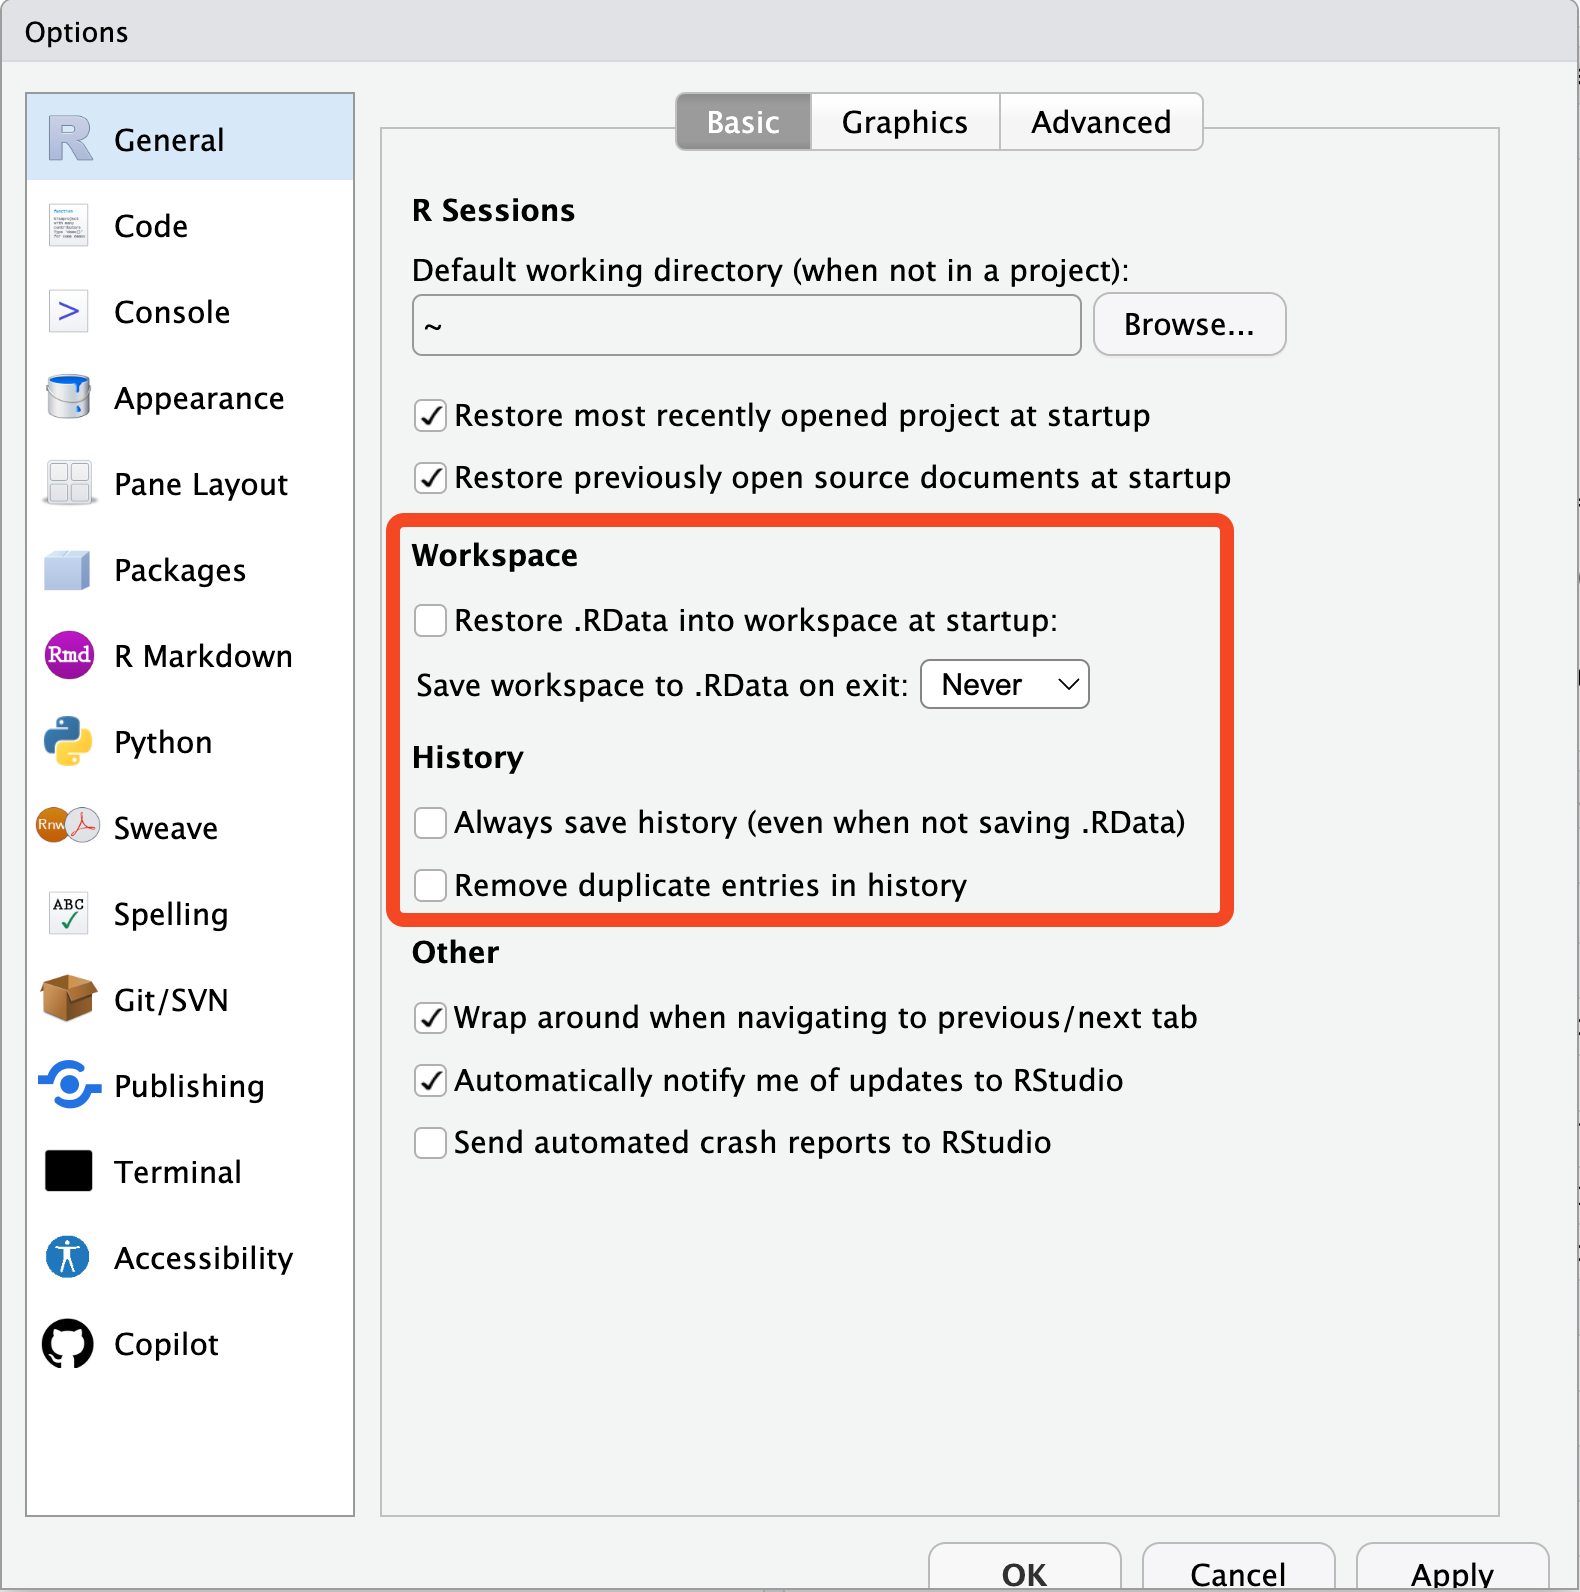
\includegraphics[width=0.7\linewidth,height=\textheight,keepaspectratio]{figs/rstudio-remove-data.png}

\emph{Setting the options so you neither restore nor save your previous
session's work.}

\section{Positron}

The same settings live under Settings → Extensions → R. The equivalent
behaviour is off by default, so there is usually nothing to change ---
but it is worth looking, so you know where it is.

This matters for two reasons:

\begin{enumerate}
\def\labelenumi{\arabic{enumi}.}
\tightlist
\item
  \textbf{Reproducibility.} You don't want objects from last week
  cluttering your session, and you don't want an analysis that only
  works because of one of them.
\item
  \textbf{Privacy.} You don't want private data written into a
  \texttt{.RData} file on disk as a side effect of quitting. You want to
  read data in, deliberately, every time.
\end{enumerate}

Your history is the list of commands you have typed. Not saving it means
you won't come to rely on something you typed in a previous session ---
which is a good habit to build.

You can also do this from code:

\begin{Shaded}
\begin{Highlighting}[]
\NormalTok{usethis}\SpecialCharTok{::}\FunctionTok{use\_blank\_slate}\NormalTok{()}
\end{Highlighting}
\end{Shaded}

With that set, restarting R gives you a genuinely clean session. The
keyboard shortcut is worth memorising:

\begin{itemize}
\tightlist
\item
  \textbf{Restart R}: \texttt{Cmd/Ctrl\ +\ Shift\ +\ F10}
\end{itemize}

The habit that goes with it: \textbf{restart R often, and re-run your
script from the top.} If it works from a clean session, it works. If it
only works in your current session, you have a bug that hasn't happened
yet.

This is also the single cheapest check that your project is portable.

Running your scripts in a clean environment is how you find out whether
the code quietly depends on something that only exists on your machine.
An object you made by hand, a package you loaded and forgot, or your own
folder layout.

Nobody else has any of those.

While you are in the settings, two more worth turning on:

\begin{itemize}
\tightlist
\item
  \textbf{Show line numbers} --- you cannot discuss code you cannot
  point at.
\item
  \textbf{Rainbow parentheses} --- cheap insurance against a very common
  class of error.
\end{itemize}

\begin{tcolorbox}[enhanced jigsaw, arc=.35mm, bottomrule=.15mm, bottomtitle=1mm, breakable, colback=white, colbacktitle=quarto-callout-note-color!10!white, colframe=quarto-callout-note-color-frame, coltitle=black, left=2mm, leftrule=.75mm, opacityback=0, opacitybacktitle=0.6, rightrule=.15mm, title=\textcolor{quarto-callout-note-color}{\faInfo}\hspace{0.5em}{Your Turn}, titlerule=0mm, toprule=.15mm, toptitle=1mm]

\begin{enumerate}
\def\labelenumi{\arabic{enumi}.}
\tightlist
\item
  Turn off workspace saving using the settings above, or run
  \texttt{usethis::use\_blank\_slate()}.
\item
  Restart R with \texttt{Cmd/Ctrl\ +\ Shift\ +\ F10}.
\item
  Open your most recent analysis script and run it from the top in the
  clean session.
\item
  Did it work? If not --- and it very often does not --- that gap is
  exactly what the rest of this course is about.
\end{enumerate}

\end{tcolorbox}

\section{Summary}\label{summary}

\begin{itemize}
\tightlist
\item
  You are always collaborating with your future self.
\item
  A file path is the address of a file; absolute paths only work on one
  machine.
\item
  Use one folder and one \texttt{.Rproj} per project, and relative paths
  within it.
\item
  \texttt{here::here()} builds paths from the project root, wherever the
  code is called from.
\item
  Raw data is read-only; output is disposable.
\item
  Make the running order obvious.
\item
  Write a README that says what, how, and where from.
\item
  Start R with a blank slate, and restart often.
\end{itemize}

Next, we will look at what happens \emph{inside} those files: how code
is styled, and why consistency makes code readable.

\bookmarksetup{startatroot}

\chapter{Code style and readability}\label{code-style-and-readability-1}

There is more to your code than having it run. I mean, it \emph{should
run}, and that is the first step. But this is a book on \emph{best
practices}, so we are actually aiming for your code to be not just
``running'', but ``easy to read, and easy to understand''.

There are some really useful tools we can apply to get quick wins on
improving the readability of your code. In this section we will discuss
concepts of \emph{code style}, talking about how to easily improve code
\emph{layout (whitespace, newlines, punctuation standards)}, and
improving code with \emph{code linting} - where a program looks at how
your code is written and identifies common errors, style
inconsistencies, and other known problem patterns.

\section{Overview}\label{overview-1}

\begin{itemize}
\tightlist
\item
  \textbf{Duration} 45 minutes
\end{itemize}

\section{Questions}\label{questions-1}

\begin{itemize}
\tightlist
\item
  Why does style matter?
\item
  What is a code formatter?
\item
  What is a code linter?
\end{itemize}

\section{Reading things that are hard to
read}\label{reading-things-that-are-hard-to-read}

Which of these is easier to read?

\begin{quote}
I am so clever that sometimes I don't understand a single word of what I
am saying
\end{quote}

And

\begin{quote}
i dont understan an ingle werd sumtimes of wot i say, but it is becoz i
am so cleva
\end{quote}

(from Oscar Wilde, The Happy Prince and Other Stories)

I've called this section: ``Reading things that are hard to read'', and
the point of the above is that one of these is harder to read than the
other, and I think this is because the second one has a few spelling
mistakes, and doesn't clearly express what it says.

Now, writing is hard! I'm not saying it is easy. It takes time, it takes
iteration. You have to revisit things. But the point is that when the
spelling is correct, and the grammar is good, it is easier to read and
understand than when it isn't.

Punctuation does the same job, and sometimes it does more than that.
Sometimes it decides what the words mean.

Here is Lionel Hutz, attorney at law.

\section{The card}


\includegraphics[width=0.7\linewidth,height=\textheight,keepaspectratio]{figs/lionel-hutz-card-clean.png}

Works on contingency, no money down. Sounds like a reasonable offer.

\section{Marked up}


\includegraphics[width=0.7\linewidth,height=\textheight,keepaspectratio]{figs/lionel-hutz-card.png}

Three marks in red pen, and not one word has changed.

Works on contingency? No, money down!

The point of the above is that you can still work out what it says. But
you spend energy doing it. Our precious mental energy. If you're reading
something and these little bumps interrupt your thinking:

\begin{itemize}
\tightlist
\item
  silently correcting correcting ``their'' to ``there''.
\item
  Has a sentence ended? There was a capital letter.
\item
  re-reading the sentence, it sounds backwards.
\end{itemize}

Our energy and our attention are finite resources, and if we spend them
on these smaller things, then we will spend less energy on the goal:
understanding the meaning.

\subsection{Mental cycles}\label{mental-cycles}

I find it useful to borrow a word from computers here, and talk about
\textbf{mental cycles}.

A computer has CPU cycles. We spend a lot of effort saving them. We
vectorise a loop, we avoid making a copy of a big object, we shave
milliseconds off something that runs a thousand times.

You have mental cycles too, and yours are much more expensive.

So here is the trade I want you to notice. Say some very terse code
saves the computer a tenth of a second, but it takes you an extra minute
or two to read it every time you come back. You have not made anything
faster. You have moved the cost off the machine, which has cycles to
spare, and onto yourself, who does not.

\textbf{Removing mental cycles is usually worth more than removing
computer cycles.}

Spend the computer's freely. Guard your own.

My point is that code is the same.

In fact R has its own version of the Hutz card:

\begin{Shaded}
\begin{Highlighting}[]
\NormalTok{x }\OtherTok{\textless{}{-}} \DecValTok{1}
\NormalTok{x }\SpecialCharTok{\textless{}} \SpecialCharTok{{-}}\DecValTok{1}
\end{Highlighting}
\end{Shaded}

\begin{verbatim}
[1] FALSE
\end{verbatim}

The first line assigns \texttt{1} to \texttt{x}. The second asks whether
\texttt{x} is less than negative one. One space, and a completely
different meaning.

R accepted both without complaint, which is the whole problem.

Compare these two:

\begin{Shaded}
\begin{Highlighting}[]
\NormalTok{d}\OtherTok{\textless{}{-}}\NormalTok{ChickWeight;d}\OtherTok{\textless{}{-}}\NormalTok{d[d}\SpecialCharTok{$}\NormalTok{Time}\SpecialCharTok{==}\DecValTok{21}\NormalTok{,];M}\OtherTok{\textless{}{-}}\FunctionTok{mean}\NormalTok{(d}\SpecialCharTok{$}\NormalTok{weight);S}\OtherTok{\textless{}{-}}\FunctionTok{sd}\NormalTok{(d}\SpecialCharTok{$}\NormalTok{weight);}\FunctionTok{c}\NormalTok{(M,S)}
\end{Highlighting}
\end{Shaded}

\begin{verbatim}
[1] 218.68889  71.51027
\end{verbatim}

\begin{Shaded}
\begin{Highlighting}[]
\NormalTok{chicks\_day\_21 }\OtherTok{\textless{}{-}}\NormalTok{ ChickWeight[ChickWeight}\SpecialCharTok{$}\NormalTok{Time }\SpecialCharTok{==} \DecValTok{21}\NormalTok{, ]}
\NormalTok{weight\_mean }\OtherTok{\textless{}{-}} \FunctionTok{mean}\NormalTok{(chicks\_day\_21}\SpecialCharTok{$}\NormalTok{weight)}
\NormalTok{weight\_sd }\OtherTok{\textless{}{-}} \FunctionTok{sd}\NormalTok{(chicks\_day\_21}\SpecialCharTok{$}\NormalTok{weight)}
\FunctionTok{c}\NormalTok{(weight\_mean, weight\_sd)}
\end{Highlighting}
\end{Shaded}

\begin{verbatim}
[1] 218.68889  71.51027
\end{verbatim}

Both of these will run. R does not care where you put your spaces. R
does not care that your variables are short, that your code is very long
winded.

But you care about these things - every stray space, and ever
inconsistent name is one more small correction you make before you can
get at what the code is trying to do.

You are spending your mental cycles on this problem. It would be nice if
you didn't have to do that.

And that is part of what this lesson is about - there are ways to
automate a lot of this! And there are ways to turn the rest into a
habit, so it stops being a decision you make every time you write a
line.

Here's the good news. Nearly all of that surface level noise is
systematic, which means we can get rid of it systematically. Quite a lot
of it we can hand to a computer entirely.

And once it's gone, your attention goes to the part that actually needs
you: whether the code does the right thing.

\section{Style is like grammar}\label{style-is-like-grammar}

Style guides define a set of rules that keep code easy to read. To quote
\href{https://hadley.nz/}{Hadley Wickham}:

\begin{quote}
Good coding style is like correct punctuation: you can manage without
it, butitsuremakesthingseasiertoread.
\end{quote}

That's the whole argument, and the sentence performs it on you as you
read it.

There is a comprehensive guide in the
\href{https://style.tidyverse.org/}{Tidyverse style guide}, and a
shorter one in the \href{http://adv-r.had.co.nz/Style.html}{style
chapter of Advanced R, 1st edition}.

\subsection{Style: layout, naming,
correctness}\label{style-layout-naming-correctness}

It helps to split ``style'' into two parts, because they need very
different things from you.

\textbf{Layout.} Where the spaces go, where the line breaks go, how deep
the indentation is, how a long function call gets split across lines.

\begin{Shaded}
\begin{Highlighting}[]
\CommentTok{\# layout}
\FunctionTok{mean}\NormalTok{(x,}\AttributeTok{na.rm=}\ConstantTok{TRUE}\NormalTok{)}
\FunctionTok{mean}\NormalTok{(x, }\AttributeTok{na.rm =} \ConstantTok{TRUE}\NormalTok{)}
\end{Highlighting}
\end{Shaded}

This part is completely mechanical, and a tool can do all of it.

\textbf{Naming.} What you call your variables, your functions, and your
files.

\begin{Shaded}
\begin{Highlighting}[]
\CommentTok{\# naming}
\NormalTok{d2 }\OtherTok{\textless{}{-}}\NormalTok{ d[d}\SpecialCharTok{$}\NormalTok{Time }\SpecialCharTok{==} \DecValTok{21}\NormalTok{, ]}
\NormalTok{chicks\_day\_21 }\OtherTok{\textless{}{-}}\NormalTok{ ChickWeight[ChickWeight}\SpecialCharTok{$}\NormalTok{Time }\SpecialCharTok{==} \DecValTok{21}\NormalTok{, ]}
\end{Highlighting}
\end{Shaded}

No tool can do this for you, because a name is a decision about meaning.

There is a third thing that is not style at all, but often gets lumped
in with it.

\textbf{Correctness.} Whether your code actually does what you think it
does.

\begin{Shaded}
\begin{Highlighting}[]
\CommentTok{\# correctness}
\ControlFlowTok{if}\NormalTok{ (}\FunctionTok{all.equal}\NormalTok{(x, y)) }\StringTok{"same"} \ControlFlowTok{else} \StringTok{"different"}
\ControlFlowTok{if}\NormalTok{ (}\FunctionTok{isTRUE}\NormalTok{(}\FunctionTok{all.equal}\NormalTok{(x, y))) }\StringTok{"same"} \ControlFlowTok{else} \StringTok{"different"}
\end{Highlighting}
\end{Shaded}

Both of those are laid out perfectly well. Only one of them is right,
and we come back to why later in this chapter. That is a \emph{linter's}
job.

So.

\begin{itemize}
\tightlist
\item
  Layout is automatable
\item
  Naming is yours
\item
  Correctness is a different tool
\end{itemize}

\begin{figure}[ht]

{\centering 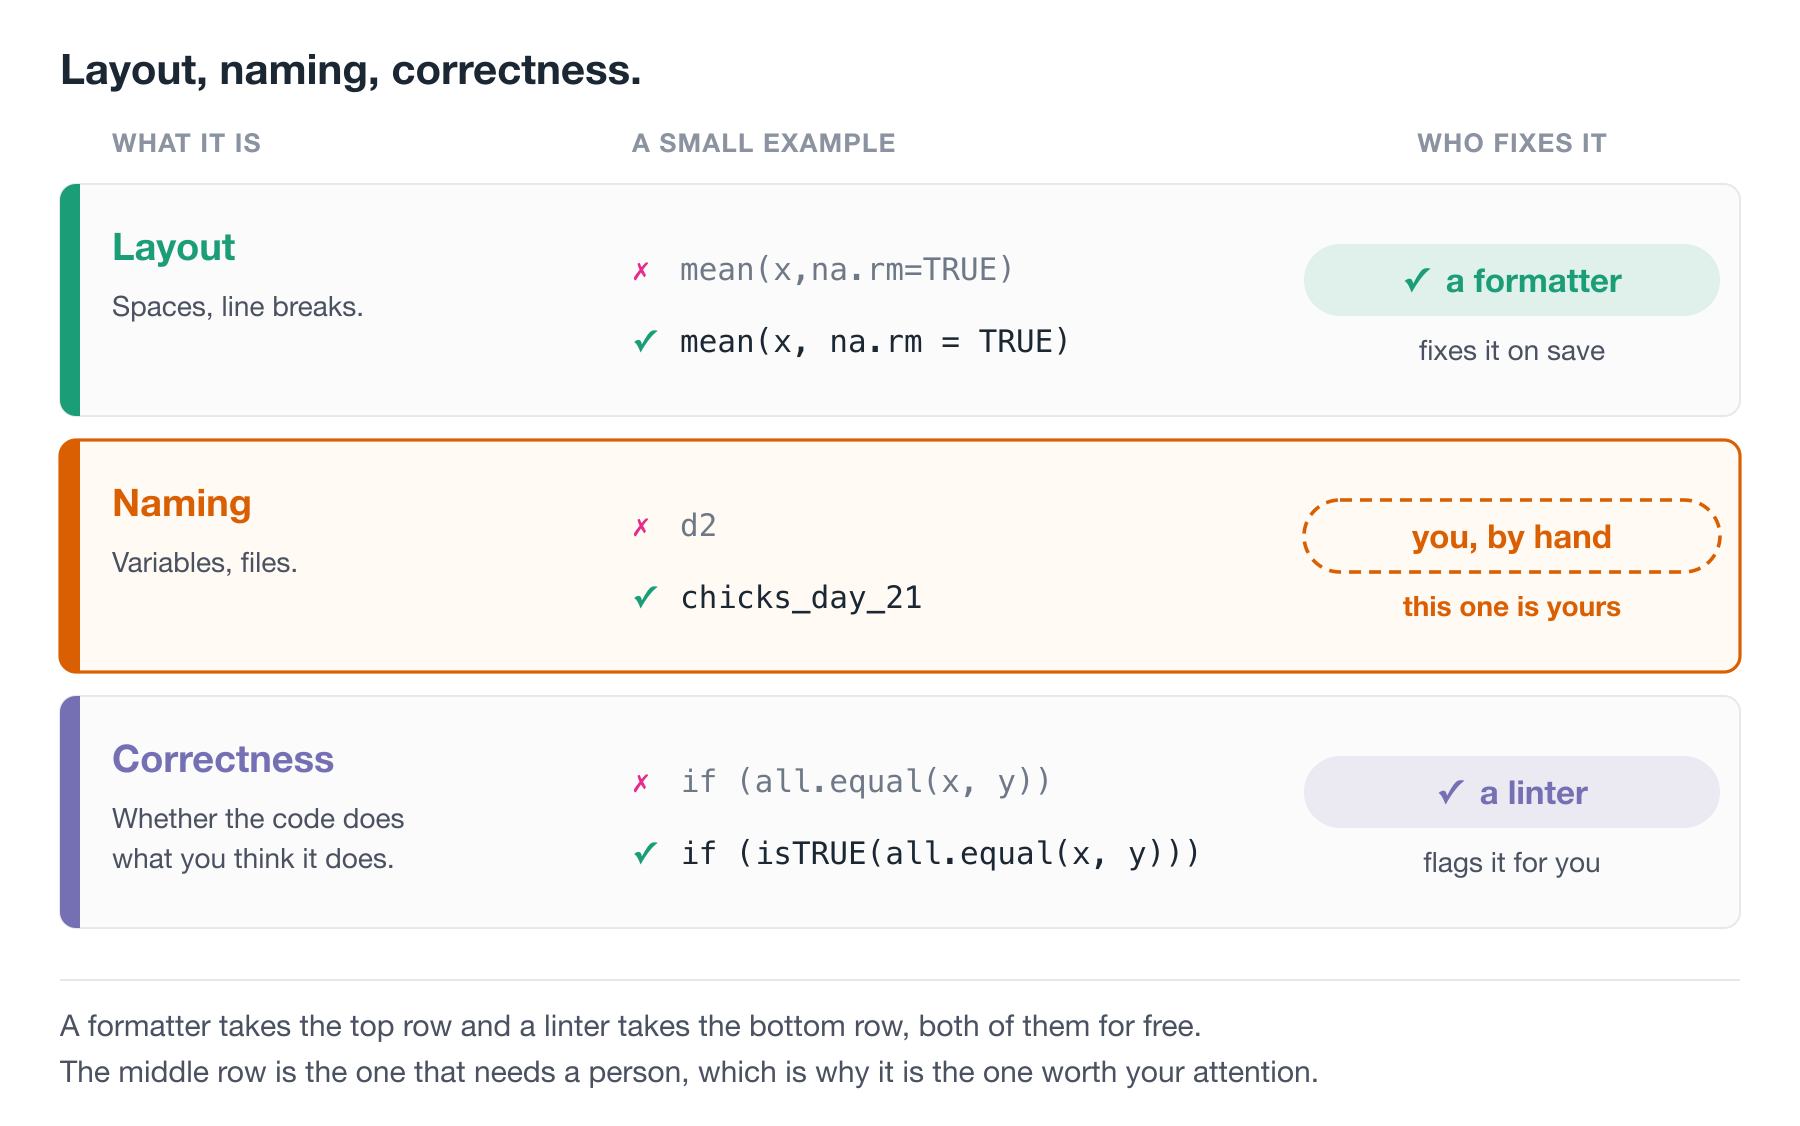
\includegraphics[width=1\linewidth,height=\textheight,keepaspectratio,alt={Three rows, each with an example and the thing that fixes it. Layout, where the spaces and line breaks go: mean(x,na.rm=TRUE) becomes mean(x, na.rm = TRUE), and air, a formatter, fixes it on save. Naming, what you call your variables and your files: d2 becomes chicks\_day\_21, and the row is outlined in orange with a dashed badge reading you, by hand, because no tool can do this. Correctness, whether the code does what you think it does: if (all.equal(x, y)) becomes if (isTRUE(all.equal(x, y))), and jarl, a linter, flags it for you. The middle row is the gap the tools cannot fill.}]{figs/style-three-jobs.png}

}

\caption{A formatter takes the layout and a linter takes the
correctness. The naming in the middle is the one with no tool.}

\end{figure}%

Let's get into it.

\section{Layout}\label{layout}

Let's look at the same code twice.

\section{Hard work}

\begin{Shaded}
\begin{Highlighting}[]
\NormalTok{penguin\_summary}\OtherTok{\textless{}{-}}\NormalTok{penguins}\SpecialCharTok{|\textgreater{}}\FunctionTok{filter}\NormalTok{(}\SpecialCharTok{!}\FunctionTok{is.na}\NormalTok{(bill\_len))}\SpecialCharTok{|\textgreater{}}\FunctionTok{group\_by}\NormalTok{(species,island)}\SpecialCharTok{|\textgreater{}}
\FunctionTok{summarise}\NormalTok{(}\AttributeTok{bill\_mean=}\FunctionTok{mean}\NormalTok{(bill\_len),}\AttributeTok{bill\_sd=}\FunctionTok{sd}\NormalTok{(bill\_len),}\AttributeTok{n=}\FunctionTok{n}\NormalTok{())}
\end{Highlighting}
\end{Shaded}

\section{Easy work}

\begin{Shaded}
\begin{Highlighting}[]
\NormalTok{penguin\_summary }\OtherTok{\textless{}{-}}\NormalTok{ penguins }\SpecialCharTok{|\textgreater{}}
  \FunctionTok{filter}\NormalTok{(}\SpecialCharTok{!}\FunctionTok{is.na}\NormalTok{(bill\_len)) }\SpecialCharTok{|\textgreater{}}
  \FunctionTok{group\_by}\NormalTok{(species, island) }\SpecialCharTok{|\textgreater{}}
  \FunctionTok{summarise}\NormalTok{(}
    \AttributeTok{bill\_mean =} \FunctionTok{mean}\NormalTok{(bill\_len),}
    \AttributeTok{bill\_sd =} \FunctionTok{sd}\NormalTok{(bill\_len),}
    \AttributeTok{n =} \FunctionTok{n}\NormalTok{()}
\NormalTok{  )}
\end{Highlighting}
\end{Shaded}

Both give the same answer. R sees no difference at all.

But in the second one you can see the shape of the analysis:

\begin{itemize}
\tightlist
\item
  filter()
\item
  group\_by()
\item
  summarise()
\end{itemize}

Three steps, one per line, each indented to show it belongs to the
pipeline.

In the first one you have to parse it yourself, character by character,
before you can even start thinking about whether the analysis is right.

\begin{tcolorbox}[enhanced jigsaw, arc=.35mm, bottomrule=.15mm, bottomtitle=1mm, breakable, colback=white, colbacktitle=quarto-callout-note-color!10!white, colframe=quarto-callout-note-color-frame, coltitle=black, left=2mm, leftrule=.75mm, opacityback=0, opacitybacktitle=0.6, rightrule=.15mm, title=\textcolor{quarto-callout-note-color}{\faInfo}\hspace{0.5em}{Your Turn}, titlerule=0mm, toprule=.15mm, toptitle=1mm]

Take this and work out, by reading alone, what it produces:

\begin{Shaded}
\begin{Highlighting}[]
\NormalTok{x}\OtherTok{\textless{}{-}}\FunctionTok{lm}\NormalTok{(body\_mass}\SpecialCharTok{\textasciitilde{}}\NormalTok{flipper\_len}\SpecialCharTok{+}\NormalTok{species,}\AttributeTok{data=}\NormalTok{penguins[penguins}\SpecialCharTok{$}\NormalTok{year}\SpecialCharTok{==}\DecValTok{2008}\SpecialCharTok{\&!}\FunctionTok{is.na}\NormalTok{(penguins}\SpecialCharTok{$}\NormalTok{sex),])}
\end{Highlighting}
\end{Shaded}

\begin{enumerate}
\def\labelenumi{\arabic{enumi}.}
\tightlist
\item
  How many things are being filtered out?
\item
  What is the response variable?
\item
  How long did that take you?
\end{enumerate}

\end{tcolorbox}

\subsection{The one line special}\label{the-one-line-special}

I once saw someone writing code where the goal, as far as I could tell,
was to have as few lines as possible.

Not fewer \emph{steps}. Fewer \emph{lines}.

It was an entire analysis. Read the data in, reshape it, fit a model,
draw a plot, save it. Four lines.

Have a look at both of these, and see which one you would rather open on
a Monday morning.

\section{Four lines}

\begin{Shaded}
\begin{Highlighting}[]
\NormalTok{penguins }\OtherTok{\textless{}{-}} \FunctionTok{read\_csv}\NormalTok{(}\StringTok{"data/penguins.csv"}\NormalTok{) }\SpecialCharTok{|\textgreater{}} \FunctionTok{filter}\NormalTok{(}\SpecialCharTok{!}\FunctionTok{is.na}\NormalTok{(bill\_length\_mm), }\SpecialCharTok{!}\FunctionTok{is.na}\NormalTok{(body\_mass\_g)) }\SpecialCharTok{|\textgreater{}} \FunctionTok{mutate}\NormalTok{(}\AttributeTok{mass\_kg =}\NormalTok{ body\_mass\_g }\SpecialCharTok{/} \DecValTok{1000}\NormalTok{, }\AttributeTok{bill\_ratio =}\NormalTok{ bill\_length\_mm }\SpecialCharTok{/}\NormalTok{ bill\_depth\_mm) }\SpecialCharTok{|\textgreater{}} \FunctionTok{group\_by}\NormalTok{(species) }\SpecialCharTok{|\textgreater{}} \FunctionTok{mutate}\NormalTok{(}\AttributeTok{mass\_z =}\NormalTok{ (mass\_kg }\SpecialCharTok{{-}} \FunctionTok{mean}\NormalTok{(mass\_kg)) }\SpecialCharTok{/} \FunctionTok{sd}\NormalTok{(mass\_kg)) }\SpecialCharTok{|\textgreater{}} \FunctionTok{ungroup}\NormalTok{()}
\NormalTok{fit }\OtherTok{\textless{}{-}} \FunctionTok{lm}\NormalTok{(mass\_kg }\SpecialCharTok{\textasciitilde{}}\NormalTok{ bill\_ratio }\SpecialCharTok{+}\NormalTok{ species }\SpecialCharTok{+}\NormalTok{ island, }\AttributeTok{data =}\NormalTok{ penguins)}
\NormalTok{p }\OtherTok{\textless{}{-}} \FunctionTok{ggplot}\NormalTok{(penguins, }\FunctionTok{aes}\NormalTok{(}\AttributeTok{x =}\NormalTok{ bill\_ratio, }\AttributeTok{y =}\NormalTok{ mass\_kg, }\AttributeTok{colour =}\NormalTok{ species)) }\SpecialCharTok{+} \FunctionTok{geom\_point}\NormalTok{(}\AttributeTok{alpha =} \FloatTok{0.6}\NormalTok{) }\SpecialCharTok{+} \FunctionTok{geom\_smooth}\NormalTok{(}\AttributeTok{method =} \StringTok{"lm"}\NormalTok{, }\AttributeTok{se =} \ConstantTok{FALSE}\NormalTok{) }\SpecialCharTok{+} \FunctionTok{facet\_wrap}\NormalTok{(}\SpecialCharTok{\textasciitilde{}}\NormalTok{island) }\SpecialCharTok{+} \FunctionTok{labs}\NormalTok{(}\AttributeTok{x =} \StringTok{"Bill length / bill depth"}\NormalTok{, }\AttributeTok{y =} \StringTok{"Body mass (kg)"}\NormalTok{) }\SpecialCharTok{+} \FunctionTok{theme\_minimal}\NormalTok{(}\AttributeTok{base\_size =} \DecValTok{12}\NormalTok{)}
\FunctionTok{ggsave}\NormalTok{(}\StringTok{"output/figures/mass{-}bill{-}ratio.png"}\NormalTok{, p, }\AttributeTok{width =} \DecValTok{8}\NormalTok{, }\AttributeTok{height =} \DecValTok{5}\NormalTok{, }\AttributeTok{dpi =} \DecValTok{300}\NormalTok{)}
\end{Highlighting}
\end{Shaded}

\section{The same thing, laid out}

\begin{Shaded}
\begin{Highlighting}[]
\NormalTok{penguins }\OtherTok{\textless{}{-}} \FunctionTok{read\_csv}\NormalTok{(}\StringTok{"data/penguins.csv"}\NormalTok{) }\SpecialCharTok{|\textgreater{}}
  \FunctionTok{filter}\NormalTok{(}
    \SpecialCharTok{!}\FunctionTok{is.na}\NormalTok{(bill\_length\_mm),}
    \SpecialCharTok{!}\FunctionTok{is.na}\NormalTok{(body\_mass\_g)}
\NormalTok{  ) }\SpecialCharTok{|\textgreater{}}
  \FunctionTok{mutate}\NormalTok{(}
    \AttributeTok{mass\_kg =}\NormalTok{ body\_mass\_g }\SpecialCharTok{/} \DecValTok{1000}\NormalTok{,}
    \AttributeTok{bill\_ratio =}\NormalTok{ bill\_length\_mm }\SpecialCharTok{/}\NormalTok{ bill\_depth\_mm}
\NormalTok{  ) }\SpecialCharTok{|\textgreater{}}
  \FunctionTok{group\_by}\NormalTok{(species) }\SpecialCharTok{|\textgreater{}}
  \FunctionTok{mutate}\NormalTok{(}\AttributeTok{mass\_z =}\NormalTok{ (mass\_kg }\SpecialCharTok{{-}} \FunctionTok{mean}\NormalTok{(mass\_kg)) }\SpecialCharTok{/} \FunctionTok{sd}\NormalTok{(mass\_kg)) }\SpecialCharTok{|\textgreater{}}
  \FunctionTok{ungroup}\NormalTok{()}

\NormalTok{fit }\OtherTok{\textless{}{-}} \FunctionTok{lm}\NormalTok{(mass\_kg }\SpecialCharTok{\textasciitilde{}}\NormalTok{ bill\_ratio }\SpecialCharTok{+}\NormalTok{ species }\SpecialCharTok{+}\NormalTok{ island, }\AttributeTok{data =}\NormalTok{ penguins)}

\NormalTok{p }\OtherTok{\textless{}{-}} \FunctionTok{ggplot}\NormalTok{(penguins, }\FunctionTok{aes}\NormalTok{(}\AttributeTok{x =}\NormalTok{ bill\_ratio, }\AttributeTok{y =}\NormalTok{ mass\_kg, }\AttributeTok{colour =}\NormalTok{ species)) }\SpecialCharTok{+}
  \FunctionTok{geom\_point}\NormalTok{(}\AttributeTok{alpha =} \FloatTok{0.6}\NormalTok{) }\SpecialCharTok{+}
  \FunctionTok{geom\_smooth}\NormalTok{(}\AttributeTok{method =} \StringTok{"lm"}\NormalTok{, }\AttributeTok{se =} \ConstantTok{FALSE}\NormalTok{) }\SpecialCharTok{+}
  \FunctionTok{facet\_wrap}\NormalTok{(}\SpecialCharTok{\textasciitilde{}}\NormalTok{island) }\SpecialCharTok{+}
  \FunctionTok{labs}\NormalTok{(}
    \AttributeTok{x =} \StringTok{"Bill length / bill depth"}\NormalTok{,}
    \AttributeTok{y =} \StringTok{"Body mass (kg)"}
\NormalTok{  ) }\SpecialCharTok{+}
  \FunctionTok{theme\_minimal}\NormalTok{(}\AttributeTok{base\_size =} \DecValTok{12}\NormalTok{)}

\FunctionTok{ggsave}\NormalTok{(}
  \StringTok{"output/figures/mass{-}bill{-}ratio.png"}\NormalTok{,}
\NormalTok{  p,}
  \AttributeTok{width =} \DecValTok{8}\NormalTok{,}
  \AttributeTok{height =} \DecValTok{5}\NormalTok{,}
  \AttributeTok{dpi =} \DecValTok{300}
\NormalTok{)}
\end{Highlighting}
\end{Shaded}

\begin{figure}[ht]

{\centering 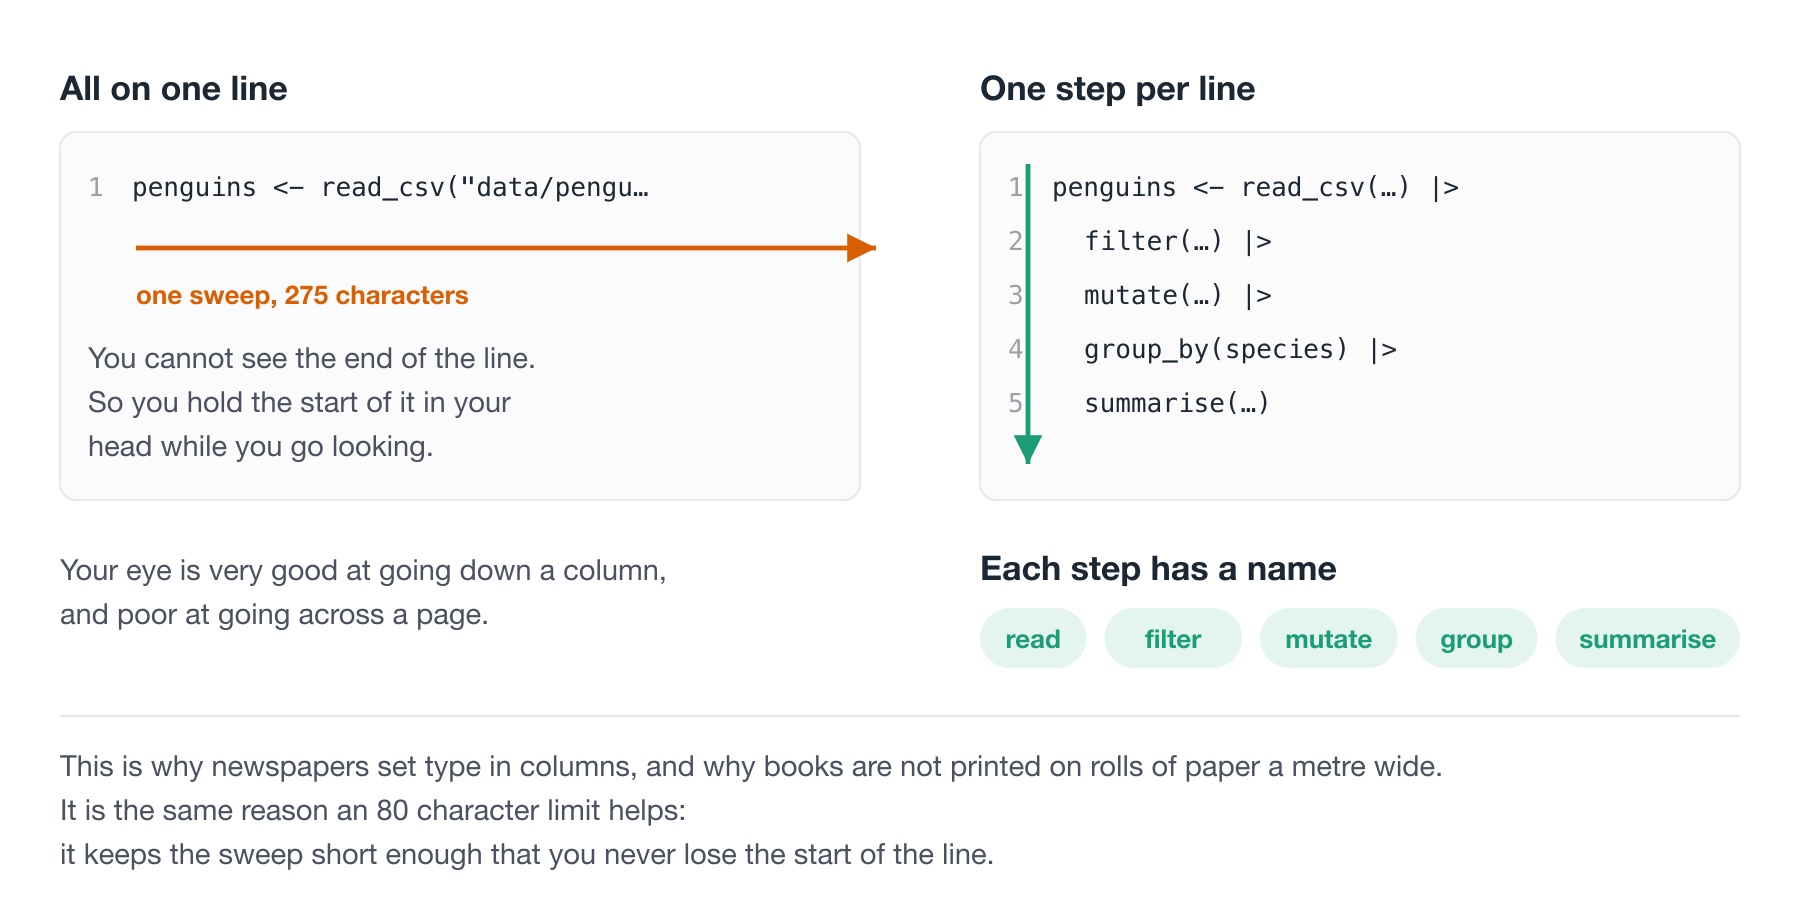
\includegraphics[width=1\linewidth,height=\textheight,keepaspectratio,alt={The same analysis two ways. As one long line the eye makes a single wide sweep and has to hold the start of the line in memory to reach the end. Broken one step per line, the eye makes five short downward steps, and each step can be named: read, filter, mutate, group, summarise.}]{figs/scan-down-not-across.png}

}

\caption{Why code reads better down a column than across a page.}

\end{figure}%

Same code. Same results.

But look at what your eye can do with the second one. You can run down
the left hand edge and read the steps off like a list: filter, mutate,
group by, mutate, ungroup.

Your eye is very good at scanning down a column. It is terrible at
scanning across a page, which is why newspapers use columns and why
books are not printed on rolls of paper a metre wide.

The first version makes you do the horizontal thing. On a laptop you
cannot even see the end of those lines without scrolling sideways, so
you are holding the start of the line in your head while you go looking
for the end of it.

Those are mental cycles, and you are burning them on the shape of the
code rather than on the analysis.

There is a second thing that shows up the moment something breaks. R
tells you which line the error is on. In the first version that is not
much help, because a quarter of your analysis is on that line.

Lines are free. Use them.

\section{Naming}\label{naming}

This is the half of style that a formatter cannot help you with.

Pick a convention, \texttt{snake\_case}, \texttt{camelCase}, or
\texttt{CamelCase}, and stick to it. I prefer \texttt{snake\_case}
because I find it easier to read, but the choice matters far less than
the consistency.

Consistency matters for a reason more concrete than tidiness. Compare:

\begin{Shaded}
\begin{Highlighting}[]
\NormalTok{weight\_mean }\OtherTok{\textless{}{-}} \FunctionTok{mean}\NormalTok{(ChickWeight}\SpecialCharTok{$}\NormalTok{weight)}
\NormalTok{sd\_weight }\OtherTok{\textless{}{-}} \FunctionTok{sd}\NormalTok{(ChickWeight}\SpecialCharTok{$}\NormalTok{weight)}
\end{Highlighting}
\end{Shaded}

with:

\begin{Shaded}
\begin{Highlighting}[]
\NormalTok{weight\_mean }\OtherTok{\textless{}{-}} \FunctionTok{mean}\NormalTok{(ChickWeight}\SpecialCharTok{$}\NormalTok{weight)}
\NormalTok{weight\_sd }\OtherTok{\textless{}{-}} \FunctionTok{sd}\NormalTok{(ChickWeight}\SpecialCharTok{$}\NormalTok{weight)}
\end{Highlighting}
\end{Shaded}

The first pair changes the order of the naming. The second sticks to one
pattern, \texttt{variable\_operation}, where the first word says what we
measured and the second says what we did to it.

Why does that help? \textbf{Tab complete.}

If I am consistent, I can type \texttt{weight\_} and press tab, and R
tells me every single thing I have done to \texttt{weight}.

If I had chosen the other order, \texttt{sd\_} would tell me everything
I have taken a standard deviation of:

\begin{Shaded}
\begin{Highlighting}[]
\NormalTok{sd\_weight }\OtherTok{\textless{}{-}} \FunctionTok{sd}\NormalTok{(ChickWeight}\SpecialCharTok{$}\NormalTok{weight)}
\NormalTok{sd\_time }\OtherTok{\textless{}{-}} \FunctionTok{sd}\NormalTok{(ChickWeight}\SpecialCharTok{$}\NormalTok{Time)}
\end{Highlighting}
\end{Shaded}

Either order is fine. What you can't do is mix them.

Because then you have to \emph{remember} which way round you named each
thing, and that's exactly the kind of small tax that makes code tiring
to work with.

\section{Consistent}

\begin{Shaded}
\begin{Highlighting}[]
\NormalTok{weight\_mean}
\NormalTok{weight\_sd}
\NormalTok{time\_mean}
\NormalTok{time\_sd}
\end{Highlighting}
\end{Shaded}

\section{Inconsistent}

\begin{Shaded}
\begin{Highlighting}[]
\NormalTok{sd\_Weight}
\NormalTok{SD\_weight}
\NormalTok{Long\_variable\_Name}
\NormalTok{timeSD}
\end{Highlighting}
\end{Shaded}

The second set is not wrong, exactly. It just means that every time you
want one of those objects you have to recall how you happened to feel on
the day you made it.

\section{Read a style guide, once}\label{read-a-style-guide-once}

It's worth your time to read through a style guide once. Properly, start
to finish, one time.

You'll notice things in your own code that you didn't see before, and
you'll see other people's code differently. It's a bit like learning
about \href{https://xkcd.com/1015/}{kerning}.

Once you see it, you notice it everywhere.

\begin{tcolorbox}[enhanced jigsaw, arc=.35mm, bottomrule=.15mm, bottomtitle=1mm, breakable, colback=white, colbacktitle=quarto-callout-note-color!10!white, colframe=quarto-callout-note-color-frame, coltitle=black, left=2mm, leftrule=.75mm, opacityback=0, opacitybacktitle=0.6, rightrule=.15mm, title=\textcolor{quarto-callout-note-color}{\faInfo}\hspace{0.5em}{Your Turn}, titlerule=0mm, toprule=.15mm, toptitle=1mm]

Read the \href{http://adv-r.had.co.nz/Style.html}{style chapter of
Advanced R, 1st edition}. It is short, and you can get through it in
about ten minutes.

As you read, keep a list of the rules you are currently breaking. Don't
fix anything yet.

\end{tcolorbox}

\begin{tcolorbox}[enhanced jigsaw, arc=.35mm, bottomrule=.15mm, bottomtitle=1mm, breakable, colback=white, colbacktitle=quarto-callout-tip-color!10!white, colframe=quarto-callout-tip-color-frame, coltitle=black, left=2mm, leftrule=.75mm, opacityback=0, opacitybacktitle=0.6, rightrule=.15mm, title=\textcolor{quarto-callout-tip-color}{\faLightbulb}\hspace{0.5em}{Going deeper}, titlerule=0mm, toprule=.15mm, toptitle=1mm]

When you have more time, read sections 1 to 5 of the
\href{https://style.tidyverse.org/}{Tidyverse style guide}: files,
syntax, functions, pipes, and ggplot2.

It is the more complete treatment, and it explains the reasoning behind
each rule rather than just stating it.

The \href{https://style.tidyverse.org/files.html}{files chapter} is
worth reading alongside the project organisation lesson, because it is
really about project structure rather than code.

\end{tcolorbox}

\section{Do I have to do all this by
hand?}\label{do-i-have-to-do-all-this-by-hand}

No.~And you shouldn't.

If you try to apply a style guide by hand you will spend your time
putting spaces after commas, lining up arguments, and re-indenting
things you just moved. It is tedious, and you will do it inconsistently,
because it is exactly the kind of task humans are bad at and get bored
by.

Worse, you'll do it \emph{instead of} the analysis.

The good news is that layout is mechanical, and mechanical things can be
automated.

\section{Using the \{air\} formatter}\label{using-the-air-formatter}

\href{https://posit-dev.github.io/air/}{Air} is an R formatter from
Posit. You point it at your code, and it lays it out properly.

It is basically magic, and it changes how you work almost immediately.

Once you have it wired into your editor, you stop thinking about layout.
You type whatever comes out of your head, hit save, and it comes out
tidy. That's it. That's the whole workflow.

\subsection{Installing air}\label{installing-air}

On macOS and Linux:

\begin{Shaded}
\begin{Highlighting}[]
\ExtensionTok{curl} \AttributeTok{{-}LsSf}\NormalTok{ https://github.com/posit{-}dev/air/releases/latest/download/air{-}installer.sh }\KeywordTok{|} \FunctionTok{sh}
\end{Highlighting}
\end{Shaded}

On Windows:

\begin{Shaded}
\begin{Highlighting}[]
\NormalTok{powershell }\OperatorTok{{-}}\NormalTok{ExecutionPolicy Bypass }\OperatorTok{{-}}\NormalTok{c }\StringTok{"irm https://github.com/posit{-}dev/air/releases/latest/download/air{-}installer.ps1 | iex"}
\end{Highlighting}
\end{Shaded}

Check it worked:

\begin{Shaded}
\begin{Highlighting}[]
\ExtensionTok{air} \AttributeTok{{-}{-}version}
\end{Highlighting}
\end{Shaded}

You should get a version number back. If you get ``command not found'',
the install didn't finish, so try it again.

\begin{tcolorbox}[enhanced jigsaw, arc=.35mm, bottomrule=.15mm, bottomtitle=1mm, breakable, colback=white, colbacktitle=quarto-callout-note-color!10!white, colframe=quarto-callout-note-color-frame, coltitle=black, left=2mm, leftrule=.75mm, opacityback=0, opacitybacktitle=0.6, rightrule=.15mm, title=\textcolor{quarto-callout-note-color}{\faInfo}\hspace{0.5em}{Your Turn: install air}, titlerule=0mm, toprule=.15mm, toptitle=1mm]

Do this one now, before we go any further, because everything in the
rest of this section needs it.

\begin{enumerate}
\def\labelenumi{\arabic{enumi}.}
\tightlist
\item
  Open a terminal. In RStudio that's the Terminal tab, next to the
  Console.
\item
  Run the install command above for your operating system.
\item
  Run \texttt{air\ -\/-version} and check you get a number.
\item
  Run \texttt{which\ air} on macOS or Linux, or \texttt{where\ air} on
  Windows, and \textbf{write the path down}. You need it in a minute.
\end{enumerate}

\end{tcolorbox}

\section{Format on save, which is the good
bit}\label{format-on-save-which-is-the-good-bit}

This is the part that changes how you work, so I want to be clear about
what it gives you.

Once this is set up, you write code however it falls out of your head.
Wonky spacing, arguments strewn across the line, indentation all over
the place. You do not fix any of it.

Then you hit \texttt{Cmd\ /\ Ctrl\ +\ S}, and it is all just correct.

Not ``you run a command and it tidies up''. You hit save, the thing you
already do a hundred times a day, and the file is formatted. There is no
new habit to build, because you are attaching it to a habit you already
have.

I cannot really oversell this. It is the single highest value setting in
this whole chapter, and it takes two minutes.

\section{RStudio}

You need RStudio 2024.12.0 or later.

You want the path you wrote down a moment ago, from \texttt{which\ air}
or \texttt{where\ air}.

Go: Tools → Global Options → Code → Formatting.

Set \textbf{Code formatter} to \textbf{External}.

Set \textbf{Reformat command} to your air path followed by
\texttt{format}, so something like
\texttt{/Users/nick/.local/bin/air\ format}. If your path has spaces in
it, wrap it in double quotes.

Now turn on format on save. Go: Tools → Global Options → Code → Saving,
and tick \textbf{Reformat documents on save}.

\section{Positron}

Air comes with Positron, so there is nothing to install.

Open the command palette (\texttt{Cmd/Ctrl\ +\ Shift\ +\ P}) and run
\textbf{Air: Initialize Workspace Folder}. This writes the recommended
settings into your project.

If you'd rather do it by hand, add this to your \texttt{settings.json}:

\begin{Shaded}
\begin{Highlighting}[]
\FunctionTok{\{}
  \DataTypeTok{"[r]"}\FunctionTok{:} \FunctionTok{\{}
    \DataTypeTok{"editor.formatOnSave"}\FunctionTok{:} \KeywordTok{true}\FunctionTok{,}
    \DataTypeTok{"editor.defaultFormatter"}\FunctionTok{:} \StringTok{"Posit.air{-}vscode"}
  \FunctionTok{\}}
\FunctionTok{\}}
\end{Highlighting}
\end{Shaded}

For R chunks inside Quarto documents, add the Quarto formatter too:

\begin{Shaded}
\begin{Highlighting}[]
\FunctionTok{\{}
  \DataTypeTok{"[quarto]"}\FunctionTok{:} \FunctionTok{\{}
    \DataTypeTok{"editor.formatOnSave"}\FunctionTok{:} \KeywordTok{true}\FunctionTok{,}
    \DataTypeTok{"editor.defaultFormatter"}\FunctionTok{:} \StringTok{"quarto.quarto"}
  \FunctionTok{\}}
\FunctionTok{\}}
\end{Highlighting}
\end{Shaded}

\begin{tcolorbox}[enhanced jigsaw, arc=.35mm, bottomrule=.15mm, bottomtitle=1mm, breakable, colback=white, colbacktitle=quarto-callout-tip-color!10!white, colframe=quarto-callout-tip-color-frame, coltitle=black, left=2mm, leftrule=.75mm, opacityback=0, opacitybacktitle=0.6, rightrule=.15mm, title=\textcolor{quarto-callout-tip-color}{\faLightbulb}\hspace{0.5em}{Setting it up from R}, titlerule=0mm, toprule=.15mm, toptitle=1mm]

If you're inside a project already, this does most of the work for you:

\begin{Shaded}
\begin{Highlighting}[]
\NormalTok{usethis}\SpecialCharTok{::}\FunctionTok{use\_air}\NormalTok{()}
\end{Highlighting}
\end{Shaded}

It sets up the editor configuration and adds an \texttt{air.toml} to
your project.

\end{tcolorbox}

\begin{tcolorbox}[enhanced jigsaw, arc=.35mm, bottomrule=.15mm, bottomtitle=1mm, breakable, colback=white, colbacktitle=quarto-callout-note-color!10!white, colframe=quarto-callout-note-color-frame, coltitle=black, left=2mm, leftrule=.75mm, opacityback=0, opacitybacktitle=0.6, rightrule=.15mm, title=\textcolor{quarto-callout-note-color}{\faInfo}\hspace{0.5em}{Your Turn: the good bit}, titlerule=0mm, toprule=.15mm, toptitle=1mm]

\begin{enumerate}
\def\labelenumi{\arabic{enumi}.}
\tightlist
\item
  Set up format on save in your editor, using the tabs above.
\item
  Open any R script. Make a mess of it on purpose. Delete the spaces
  around a \texttt{\textless{}-}, jam some arguments together, break the
  indentation.
\item
  Hit \texttt{Cmd\ /\ Ctrl\ +\ S}.
\item
  Do that three or four more times, with a different kind of mess each
  time.
\end{enumerate}

I want you to do it repeatedly, because the point is not that it worked
once. The point is to stop believing you have to tidy your own code.

\end{tcolorbox}

\subsection{On the command line}\label{on-the-command-line}

You don't need an editor at all. Air will format a single file:

\begin{Shaded}
\begin{Highlighting}[]
\ExtensionTok{air}\NormalTok{ format analysis/01{-}clean{-}data.R}
\end{Highlighting}
\end{Shaded}

or an entire project:

\begin{Shaded}
\begin{Highlighting}[]
\ExtensionTok{air}\NormalTok{ format .}
\end{Highlighting}
\end{Shaded}

That second one is the command I run most. It is also the one worth
putting in front of any code review, so that nobody spends their
attention on spacing.

\begin{tcolorbox}[enhanced jigsaw, arc=.35mm, bottomrule=.15mm, bottomtitle=1mm, breakable, colback=white, colbacktitle=quarto-callout-note-color!10!white, colframe=quarto-callout-note-color-frame, coltitle=black, left=2mm, leftrule=.75mm, opacityback=0, opacitybacktitle=0.6, rightrule=.15mm, title=\textcolor{quarto-callout-note-color}{\faInfo}\hspace{0.5em}{Your Turn}, titlerule=0mm, toprule=.15mm, toptitle=1mm]

There is a deliberately awful script in the course repository at
\texttt{06-bad-style/messy-analysis.R}. It breaks essentially every rule
in this chapter.

\begin{enumerate}
\def\labelenumi{\arabic{enumi}.}
\tightlist
\item
  Open \texttt{messy-analysis.R} and read it. Note how long it takes you
  to work out what it does.
\item
  Run \texttt{air\ format\ 06-bad-style/messy-analysis.R} from your
  terminal.
\item
  Read it again. What can you see now that you couldn't before?
\item
  Look at the variable names in the formatted version. Air has not
  touched a single one of them, and they're still a mess. Write down
  three you would rename.
\end{enumerate}

Step 4 is the important one. It's the clearest demonstration I know that
layout and naming are two different jobs.

\end{tcolorbox}

\subsection{Notes on using air}\label{notes-on-using-air}

A few things that will save you some confusion.

\textbf{There is very little to configure, and that's on purpose.} Air's
settings live in an \texttt{air.toml} file, and there are about ten of
them. The ones you might actually change are \texttt{line-width}
(default 80) and \texttt{indent-width} (default 2). There is no way to
spend an afternoon tuning it, which is the point.

\textbf{It won't work on an untitled tab.} Air needs a file that exists
on disk, with an \texttt{.R} extension, so that it knows it's looking at
R code. Save the file first.

\textbf{In RStudio it won't work inside R chunks in Quarto or R
Markdown.} This is an RStudio limitation rather than an air one, and it
may well change. Positron handles chunks fine.

\textbf{If your code doesn't reformat, you probably have a syntax
error.} Air will not format code it cannot parse. So a file that
stubbornly refuses to tidy up is telling you something useful. Go and
find your missing bracket.

That last one turns out to be a small free bonus. Format on save quietly
becomes a syntax check on save.

\section{Using linters}\label{using-linters}

Air has now taken care of how your code \emph{looks}. Here is a piece of
code where that isn't the problem.

\begin{Shaded}
\begin{Highlighting}[]
\NormalTok{sites }\OtherTok{\textless{}{-}} \FunctionTok{character}\NormalTok{(}\DecValTok{0}\NormalTok{)}

\ControlFlowTok{for}\NormalTok{ (i }\ControlFlowTok{in} \DecValTok{1}\SpecialCharTok{:}\FunctionTok{length}\NormalTok{(sites)) \{}
  \FunctionTok{message}\NormalTok{(}\StringTok{"Processing site "}\NormalTok{, sites[i])}
\NormalTok{\}}
\end{Highlighting}
\end{Shaded}

Air is perfectly happy with that. Every space is in the right place, the
indentation is correct, and running \texttt{air\ format} on it changes
nothing at all.

It is also broken.

When \texttt{sites} is empty, \texttt{length(sites)} is \texttt{0}, and
\texttt{1:0} does not give you nothing. It gives you this:

\begin{Shaded}
\begin{Highlighting}[]
\NormalTok{sites }\OtherTok{\textless{}{-}} \FunctionTok{character}\NormalTok{(}\DecValTok{0}\NormalTok{)}
\DecValTok{1}\SpecialCharTok{:}\FunctionTok{length}\NormalTok{(sites)}
\end{Highlighting}
\end{Shaded}

\begin{verbatim}
[1] 1 0
\end{verbatim}

So the loop runs twice, on elements \texttt{1} and \texttt{0}, neither
of which exists. No error, no warning, and a message about a site that
isn't there.

This is a different kind of problem, and it needs a different kind of
tool.

\begin{itemize}
\tightlist
\item
  A \textbf{formatter} changes how your code \emph{looks}.
  \texttt{\{air\}} doesn't care what your code does.
\item
  A \textbf{linter} tells you what your code might be doing
  \emph{wrong}. It reads your code without running it, which is called
  static analysis, and flags errors, bugs, and suspicious patterns.
\end{itemize}

You want both. Formatting settles arguments about layout. Linting
catches the class of mistake that runs perfectly happily and gives you
the wrong answer.

\begin{tcolorbox}[enhanced jigsaw, arc=.35mm, bottomrule=.15mm, bottomtitle=1mm, breakable, colback=white, colbacktitle=quarto-callout-caution-color!10!white, colframe=quarto-callout-caution-color-frame, coltitle=black, left=2mm, leftrule=.75mm, opacityback=0, opacitybacktitle=0.6, rightrule=.15mm, title=\textcolor{quarto-callout-caution-color}{\faFire}\hspace{0.5em}{Some history: why is it called a linter?}, titlerule=0mm, toprule=.15mm, toptitle=1mm]

The name comes from a program called \texttt{lint}, written by Stephen
C. Johnson at Bell Labs in 1978 to check C code for bugs and portability
problems. You can read more on the
\href{https://en.wikipedia.org/wiki/Lint_(software)}{Wikipedia page for
lint}.

The name is the good part. Lint is the fluff that clothes shed in the
wash, and a clothes dryer has a lint trap to catch it. Johnson's idea
was that his program would work the same way, catching the waste fibres
while leaving the fabric intact.

Your code is the fabric. The linter is the trap.

I like this because it sets the right expectation. A lint trap does not
tell you the jumper was a bad idea. It picks off the fluff, and it does
it every single load, without being asked.

\end{tcolorbox}

\subsection{jarl}\label{jarl}

\href{https://jarl.etiennebacher.com/}{Jarl}, which stands for Just
Another R Linter, is a fast linter by
\href{https://www.etiennebacher.com/}{Etienne Bacher}. It is built on
top of Air, which is why the two feel like the same tool.

Here is a script of the kind most of us have written. Nothing exotic.
Read some data in, flag a few things, print a message.

\begin{Shaded}
\begin{Highlighting}[]
\NormalTok{penguins }\OtherTok{\textless{}{-}} \FunctionTok{read.csv}\NormalTok{(}\StringTok{"data/penguins.csv"}\NormalTok{)}

\NormalTok{missing\_mass }\OtherTok{\textless{}{-}}\NormalTok{ penguins}\SpecialCharTok{$}\NormalTok{body\_mass\_g }\SpecialCharTok{==} \ConstantTok{NA}

\NormalTok{penguins}\SpecialCharTok{$}\NormalTok{heavy }\OtherTok{\textless{}{-}} \FunctionTok{ifelse}\NormalTok{(penguins}\SpecialCharTok{$}\NormalTok{body\_mass\_g }\SpecialCharTok{\textgreater{}} \DecValTok{5000}\NormalTok{, T, F)}

\NormalTok{has\_data }\OtherTok{\textless{}{-}} \FunctionTok{nrow}\NormalTok{(penguins) }\SpecialCharTok{\textgreater{}} \DecValTok{0}

\ControlFlowTok{if}\NormalTok{ (has\_data }\SpecialCharTok{==} \ConstantTok{TRUE}\NormalTok{) \{}
  \FunctionTok{message}\NormalTok{(}\StringTok{"Loaded "}\NormalTok{, }\FunctionTok{nrow}\NormalTok{(penguins), }\StringTok{" penguins"}\NormalTok{)}
\NormalTok{\}}
\end{Highlighting}
\end{Shaded}

Air has no complaints. It runs without an error.

\begin{Shaded}
\begin{Highlighting}[]
\ExtensionTok{$}\NormalTok{ jarl check penguin{-}check.R}
\end{Highlighting}
\end{Shaded}

\begin{verbatim}
warning: equals_na
 --> penguin-check.R:3:17
  |
3 | missing_mass <- penguins$body_mass_g == NA
  |                 -------------------------- Comparing to NA with `==`, `!=` or `%in%` is problematic.
  |
  = help: Use `is.na()` instead.

warning: true_false_symbol
 --> penguin-check.R:5:55
  |
5 | penguins$heavy <- ifelse(penguins$body_mass_g > 5000, T, F)
  |                                                       - `T` and `F` can be confused with variable names.
  |

warning: redundant_equals
 --> penguin-check.R:9:5
  |
9 | if (has_data == TRUE) {
  |     ---------------- Using == on a logical vector is redundant.
  |
\end{verbatim}

Let's take those one at a time, because each one teaches something.

\textbf{\texttt{missing\_mass\ \textless{}-\ penguins\$body\_mass\_g\ ==\ NA}}

This is the one I want you to remember. It looks completely reasonable,
and it is always wrong.

\texttt{NA} means ``I don't know''. So asking ``is this value equal to a
value I don't know?'' can only be answered with ``I don't know'':

\begin{Shaded}
\begin{Highlighting}[]
\NormalTok{x }\OtherTok{\textless{}{-}} \FunctionTok{c}\NormalTok{(}\DecValTok{1}\NormalTok{, }\ConstantTok{NA}\NormalTok{, }\DecValTok{3}\NormalTok{)}
\NormalTok{x }\SpecialCharTok{==} \ConstantTok{NA}
\end{Highlighting}
\end{Shaded}

\begin{verbatim}
[1] NA NA NA
\end{verbatim}

Every answer is \texttt{NA}, including for the values that are obviously
not missing. Your \texttt{missing\_mass} vector contains no information
at all, and nothing warned you.

\begin{Shaded}
\begin{Highlighting}[]
\FunctionTok{is.na}\NormalTok{(x)}
\end{Highlighting}
\end{Shaded}

\begin{verbatim}
[1] FALSE  TRUE FALSE
\end{verbatim}

That's the function you wanted.

\textbf{\texttt{ifelse(...,\ T,\ F)}}

\texttt{TRUE} and \texttt{FALSE} are reserved words in R. \texttt{T} and
\texttt{F} are just ordinary variables that happen to start out holding
\texttt{TRUE} and \texttt{FALSE}, which means anyone can reassign them.

\begin{Shaded}
\begin{Highlighting}[]
\NormalTok{T }\OtherTok{\textless{}{-}} \ConstantTok{FALSE}
\FunctionTok{mean}\NormalTok{(}\FunctionTok{c}\NormalTok{(}\DecValTok{1}\NormalTok{, }\ConstantTok{NA}\NormalTok{, }\DecValTok{3}\NormalTok{), }\AttributeTok{na.rm =}\NormalTok{ T)}
\end{Highlighting}
\end{Shaded}

\begin{verbatim}
[1] NA
\end{verbatim}

\begin{Shaded}
\begin{Highlighting}[]
\FunctionTok{rm}\NormalTok{(T)}
\end{Highlighting}
\end{Shaded}

\texttt{na.rm\ =\ T} quietly became \texttt{na.rm\ =\ FALSE}, and the
mean is now \texttt{NA}. Spell them out and this cannot happen to you.

\textbf{\texttt{if\ (has\_data\ ==\ TRUE)}}

\texttt{has\_data} is already \texttt{TRUE} or \texttt{FALSE}. Comparing
it to \texttt{TRUE} gets you back exactly what you started with, so
\texttt{if\ (has\_data)} says the same thing with less to read.

This one is not a bug. It is a mental cycles problem, which is the theme
of this whole chapter.

\begin{tcolorbox}[enhanced jigsaw, arc=.35mm, bottomrule=.15mm, bottomtitle=1mm, breakable, colback=white, colbacktitle=quarto-callout-important-color!10!white, colframe=quarto-callout-important-color-frame, coltitle=black, left=2mm, leftrule=.75mm, opacityback=0, opacitybacktitle=0.6, rightrule=.15mm, title=\textcolor{quarto-callout-important-color}{\faExclamation}\hspace{0.5em}{Two nastier ones, for later}, titlerule=0mm, toprule=.15mm, toptitle=1mm]

These turn up in real code and are much harder to spot by eye.

\texttt{class(dat)\ ==\ "data.frame"} looks fine until you meet an
object with more than one class:

\begin{Shaded}
\begin{Highlighting}[]
\FunctionTok{class}\NormalTok{(}\FunctionTok{data.frame}\NormalTok{(}\AttributeTok{x =} \DecValTok{1}\NormalTok{))}
\end{Highlighting}
\end{Shaded}

\begin{verbatim}
[1] "data.frame"
\end{verbatim}

\begin{Shaded}
\begin{Highlighting}[]
\FunctionTok{class}\NormalTok{(datasets}\SpecialCharTok{::}\NormalTok{ChickWeight)}
\end{Highlighting}
\end{Shaded}

\begin{verbatim}
[1] "nfnGroupedData" "nfGroupedData"  "groupedData"    "data.frame"    
\end{verbatim}

One class for a plain data frame, four for that one. So the comparison
hands \texttt{if()} four answers where it wanted one, and errors.
\texttt{inherits(dat,\ "data.frame")} asks the question you actually
meant.

\texttt{if\ (all.equal(x,\ y))} is worse. \texttt{all.equal()} returns
\texttt{TRUE} when things match, and a \emph{description of the
difference} when they don't:

\begin{Shaded}
\begin{Highlighting}[]
\FunctionTok{all.equal}\NormalTok{(}\DecValTok{1}\NormalTok{, }\DecValTok{1}\NormalTok{)}
\end{Highlighting}
\end{Shaded}

\begin{verbatim}
[1] TRUE
\end{verbatim}

\begin{Shaded}
\begin{Highlighting}[]
\FunctionTok{all.equal}\NormalTok{(}\DecValTok{1}\NormalTok{, }\FloatTok{1.1}\NormalTok{)}
\end{Highlighting}
\end{Shaded}

\begin{verbatim}
[1] "Mean relative difference: 0.1"
\end{verbatim}

That second one is a string, and \texttt{if()} can't do anything
sensible with it. So the code works perfectly while your values match,
and falls over the first time they don't, which is precisely the case
you wrote the check for. \texttt{isTRUE(all.equal(x,\ y))} fixes it.

\end{tcolorbox}

Notice that these fail in two different ways.

\texttt{==\ NA} and \texttt{na.rm\ =\ T} are \textbf{silent}. They run,
there is no error and no warning, and the answer is wrong.

The two in the callout above \textbf{error}, which sounds better and is
arguably worse. They work fine while the data behaves, so they pass
every test you run on tidy data, and then fail on a Friday afternoon on
somebody else's file.

That is what a linter is for. No amount of careful reading catches all
of these reliably, and a tool catches them every time in about a tenth
of a second.

Where a fix is unambiguous, jarl can apply it for you:

\begin{Shaded}
\begin{Highlighting}[]
\ExtensionTok{$}\NormalTok{ jarl check penguin{-}check.R }\AttributeTok{{-}{-}fix}
\end{Highlighting}
\end{Shaded}

which turns the \texttt{T} and \texttt{F} into \texttt{TRUE} and
\texttt{FALSE}. It won't touch the \texttt{==\ NA}, because deciding
what you actually meant there is your job, not the tool's.

It ships 55+ rules, integrates with VS Code, Positron and Zed, and runs
in CI. It's also very fast. On the \texttt{dplyr} source, roughly 25,000
lines of R, the documented benchmark is 0.131 seconds against 18.5
seconds for \texttt{\{lintr\}}.

\begin{tcolorbox}[enhanced jigsaw, arc=.35mm, bottomrule=.15mm, bottomtitle=1mm, breakable, colback=white, colbacktitle=quarto-callout-tip-color!10!white, colframe=quarto-callout-tip-color-frame, coltitle=black, left=2mm, leftrule=.75mm, opacityback=0, opacitybacktitle=0.6, rightrule=.15mm, title=\textcolor{quarto-callout-tip-color}{\faLightbulb}\hspace{0.5em}{What about lintr?}, titlerule=0mm, toprule=.15mm, toptitle=1mm]

\href{https://lintr.r-lib.org/}{\texttt{\{lintr\}}} is the long
established R linter, it's pure R, and it's what you'll meet in most
existing projects and CI setups. It's a perfectly good tool and knowing
it is worthwhile.

Jarl is newer and much faster, which matters more than it sounds.

A linter you run on every save changes your habits. A linter that takes
eighteen seconds is one you run occasionally, and then stop running.

Use whichever you like. Use one of them.

\end{tcolorbox}

\begin{tcolorbox}[enhanced jigsaw, arc=.35mm, bottomrule=.15mm, bottomtitle=1mm, breakable, colback=white, colbacktitle=quarto-callout-note-color!10!white, colframe=quarto-callout-note-color-frame, coltitle=black, left=2mm, leftrule=.75mm, opacityback=0, opacitybacktitle=0.6, rightrule=.15mm, title=\textcolor{quarto-callout-note-color}{\faInfo}\hspace{0.5em}{Your Turn}, titlerule=0mm, toprule=.15mm, toptitle=1mm]

Back to \texttt{06-bad-style/}. There's a second file there,
\texttt{dodgy-logic.R}, which is formatted perfectly well and still
wrong.

\begin{enumerate}
\def\labelenumi{\arabic{enumi}.}
\tightlist
\item
  Read it, and see if you can spot the bug by eye. Give yourself two
  minutes.
\item
  Run \texttt{jarl\ check\ 06-bad-style/dodgy-logic.R}, or
  \texttt{lintr::lint("06-bad-style/dodgy-logic.R")}.
\item
  Now run \texttt{jarl\ check} over your own most recent project. What
  comes up?
\end{enumerate}

Nothing on that last one is a judgement. I run this over my own code and
it finds things every time.

\end{tcolorbox}

\begin{tcolorbox}[enhanced jigsaw, arc=.35mm, bottomrule=.15mm, bottomtitle=1mm, breakable, colback=white, colbacktitle=quarto-callout-tip-color!10!white, colframe=quarto-callout-tip-color-frame, coltitle=black, left=2mm, leftrule=.75mm, opacityback=0, opacitybacktitle=0.6, rightrule=.15mm, title=\textcolor{quarto-callout-tip-color}{\faLightbulb}\hspace{0.5em}{Read more}, titlerule=0mm, toprule=.15mm, toptitle=1mm]

The style and naming material in this chapter is adapted from my blog
post
\href{https://www.njtierney.com/posts/2023-10-30-how-to-get-good-with-r/\#stick-to-a-style-guide}{How
to get good with R}.

\end{tcolorbox}

\section{Summary}\label{summary-1}

\begin{itemize}
\tightlist
\item
  Badly laid out code makes you spend mental cycles on the surface
  before you get to the ideas, in the same way that bad spelling does.
\item
  Mental cycles are worth more than computer cycles. Spend the
  machine's, guard your own.
\item
  Style splits into layout, which a tool can fix, and naming, which is
  yours.
\item
  Lines are free. Use them, because your eye reads down far better than
  across.
\item
  Pick a naming convention and stick to it, because consistency is what
  makes tab complete work for you.
\item
  Read a style guide once, properly, and you'll see code differently
  afterwards.
\item
  Set up \texttt{\{air\}} and format on save, then stop thinking about
  layout.
\item
  A linter is a different tool again, and it catches the bugs that run
  perfectly happily.
\end{itemize}

Next, we look at readability beyond layout: names that carry meaning,
breaking a wall of code into pieces, and how to review code.

\bookmarksetup{startatroot}

\chapter{Writing readable code}\label{writing-readable-code-1}

So far we have fixed things without really reading the code. This is the
section where we have to actually read it, and decide whether a person
can follow it.

We cover what you are looking for when you read code, a process for
reviewing it that works just as well on your own work, and how to review
someone else's without being a pain about it.

\section{Overview}\label{overview-2}

\begin{itemize}
\tightlist
\item
  \textbf{Duration} 45 minutes
\end{itemize}

\section{Questions}\label{questions-2}

\begin{itemize}
\tightlist
\item
  Where does readable code start, once the tools have done their bit?
\item
  What makes a variable name good enough?
\item
  How do I break a wall of code into readable pieces?
\item
  What am I actually looking for when I read code?
\item
  How do I review code, including my own?
\end{itemize}

\section{Where we are up to}\label{where-we-are-up-to}

Two chapters in, and you have already fixed a good deal of code without
reading any of it closely.

Chapter 1 was about where things live. A project that opens, paths that
work on someone else's machine, a README that says what the thing is.

Chapter 2 was about how the code looks. Pick a naming convention. Let
\texttt{air} handle the layout. Let a linter tell you about the rest.

Both of those are fixes you can make without understanding the analysis
at all. One is structural, and one is a button you press.

It is a bit like writing an essay.

Organising your project is putting your notes and drafts in sensible
folders. Running \texttt{air} is spell check, and running a linter is
the automatic grammar check that tells you a sentence has no verb.

All of that is useful, and none of it tells you whether the essay makes
any sense.

That is what this chapter is for. Now we read the code and ask whether a
person can follow it.

\section{Good vs bad variable names}\label{good-vs-bad-variable-names}

There is a quote attributed to \href{https://www.karlton.org/}{Phil
Karlton}:

\begin{quote}
There are only two hard things in computer science: cache invalidation
and naming things.
\end{quote}

I'm not really sure what cache invalidation is. But naming things well
is genuinely hard, and I want to lower the bar deliberately:
\textbf{giving things an OK name is much easier than giving things a
great name.} Getting into the habit of OK names is what leads, with
practice, to better ones. Aim for OK.

\begin{tcolorbox}[enhanced jigsaw, arc=.35mm, bottomrule=.15mm, bottomtitle=1mm, breakable, colback=white, colbacktitle=quarto-callout-caution-color!10!white, colframe=quarto-callout-caution-color-frame, coltitle=black, left=2mm, leftrule=.75mm, opacityback=0, opacitybacktitle=0.6, rightrule=.15mm, title=\textcolor{quarto-callout-caution-color}{\faFire}\hspace{0.5em}{Some history: where the quote comes from}, titlerule=0mm, toprule=.15mm, toptitle=1mm]

Phil Karlton was a principal developer at Xerox PARC, DEC, Silicon
Graphics and Netscape.
\href{https://martinfowler.com/bliki/TwoHardThings.html}{Martin Fowler
has written up the provenance of the quote}, which is more interesting
than you'd expect. Nobody has ever found where Karlton first said it,
and it seems to have travelled by word of mouth from about 1996.

\end{tcolorbox}

In chapter 2 we talked about naming \emph{conventions}. Pick one, stick
to it, and get tab complete for free.

This is the other half. A name can follow your convention perfectly and
still tell you nothing.

\begin{Shaded}
\begin{Highlighting}[]
\NormalTok{df1 }\OtherTok{\textless{}{-}} \FunctionTok{read.csv}\NormalTok{(}\StringTok{"survey.csv"}\NormalTok{)}
\NormalTok{df2 }\OtherTok{\textless{}{-}}\NormalTok{ df1[df1}\SpecialCharTok{$}\NormalTok{year }\SpecialCharTok{==} \DecValTok{2024}\NormalTok{, ]}
\NormalTok{df3 }\OtherTok{\textless{}{-}}\NormalTok{ df2[df2}\SpecialCharTok{$}\NormalTok{site }\SpecialCharTok{==} \StringTok{"north"}\NormalTok{, ]}
\end{Highlighting}
\end{Shaded}

That is consistent, it is \texttt{air}-clean, and a linter has no
complaint about it. But if I meet \texttt{df3} two hundred lines later I
have to go back and reconstruct what it is.

Compare:

\begin{Shaded}
\begin{Highlighting}[]
\NormalTok{survey\_raw }\OtherTok{\textless{}{-}} \FunctionTok{read.csv}\NormalTok{(}\StringTok{"survey.csv"}\NormalTok{)}
\NormalTok{survey\_2024 }\OtherTok{\textless{}{-}}\NormalTok{ survey\_raw[survey\_raw}\SpecialCharTok{$}\NormalTok{year }\SpecialCharTok{==} \DecValTok{2024}\NormalTok{, ]}
\NormalTok{survey\_north }\OtherTok{\textless{}{-}}\NormalTok{ survey\_2024[survey\_2024}\SpecialCharTok{$}\NormalTok{site }\SpecialCharTok{==} \StringTok{"north"}\NormalTok{, ]}
\end{Highlighting}
\end{Shaded}

Same code, and now the name carries the history of what happened to the
data.

There is a small counter-example. Inside very short functions,
\texttt{x} is often the right name, precisely because the function is
small enough that you can see everything at once. But that is the
exception, and you will know when you are in it.

\begin{tcolorbox}[enhanced jigsaw, arc=.35mm, bottomrule=.15mm, bottomtitle=1mm, breakable, colback=white, colbacktitle=quarto-callout-note-color!10!white, colframe=quarto-callout-note-color-frame, coltitle=black, left=2mm, leftrule=.75mm, opacityback=0, opacitybacktitle=0.6, rightrule=.15mm, title=\textcolor{quarto-callout-note-color}{\faInfo}\hspace{0.5em}{Your Turn}, titlerule=0mm, toprule=.15mm, toptitle=1mm]

\begin{enumerate}
\def\labelenumi{\arabic{enumi}.}
\tightlist
\item
  Open \texttt{07-needs-review/analysis.R} from the messy project repo.
  Find every object whose name tells you nothing about what it holds.
\item
  Rename three of them. Don't try to do all of them, and don't aim for
  perfect names. Aim for OK.
\item
  Did renaming change how long it took you to work out what the next
  section does?
\end{enumerate}

\end{tcolorbox}

\section{De-chunking code}\label{de-chunking-code}

Here is a phone number:

\begin{verbatim}
1-8-0-0-1-3-1-0-8-6
\end{verbatim}

Ten digits. Try to hold them in your head. Now try this:

\begin{verbatim}
1800 131 086
\end{verbatim}

Same ten digits, and suddenly it's easy.

Nothing about the information changed. Only the \textbf{chunking} did.

This is not a party trick. Our working memory holds roughly
\textbf{seven, plus or minus two} chunks at once, a finding from George
Miller's 1956 paper
\href{https://en.wikipedia.org/wiki/The_Magical_Number_Seven,_Plus_or_Minus_Two}{``The
magical number seven, plus or minus two''}. Crucially, memory isn't
limited by the amount of information. It's limited by the \emph{number
of chunks}.

So make bigger chunks and you hold more.

\begin{figure}[ht]

{\centering 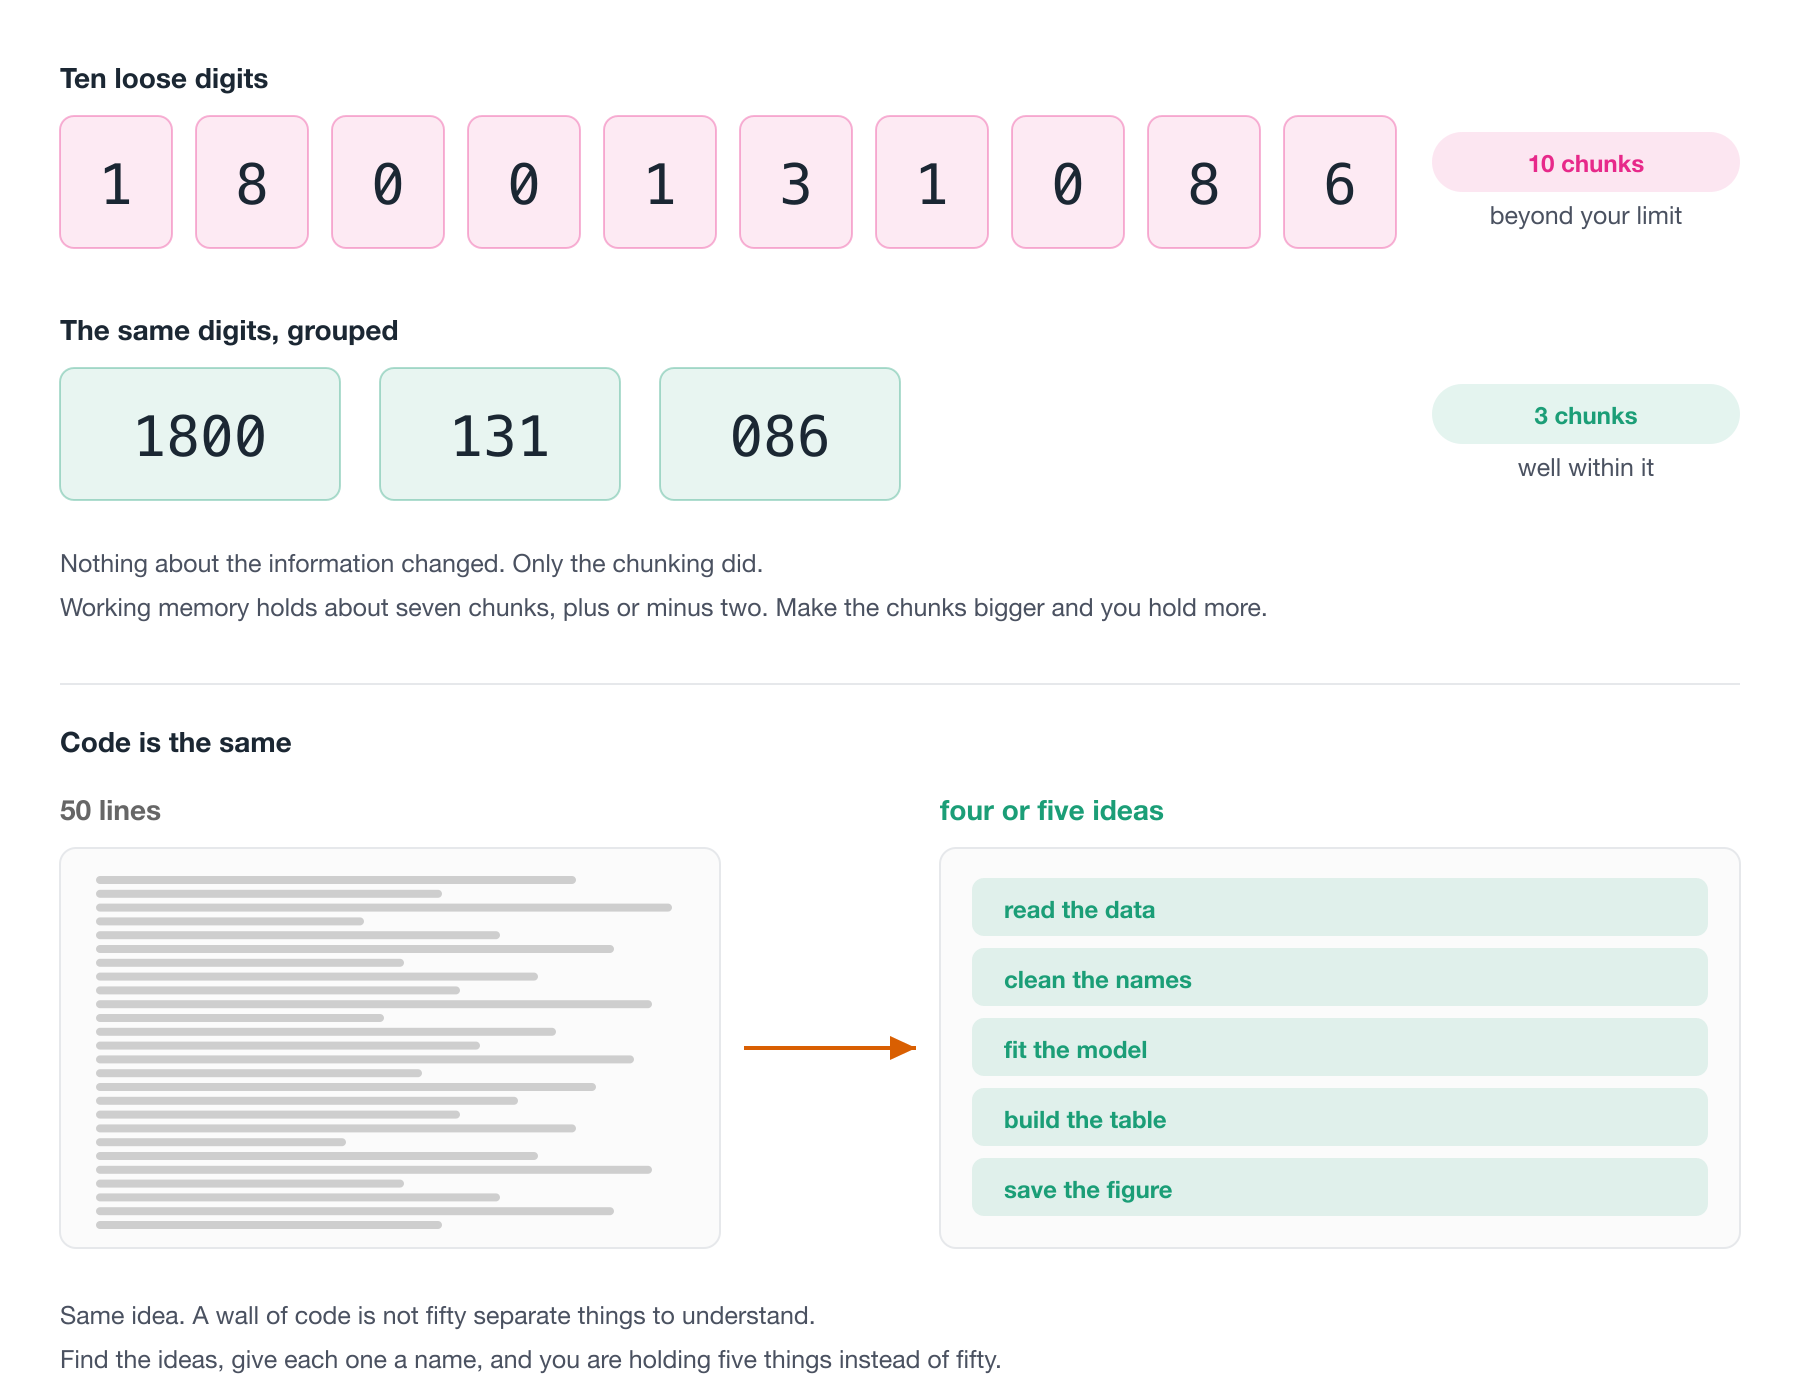
\includegraphics[width=1\linewidth,height=\textheight,keepaspectratio,alt={Ten pink boxes each holding one digit of 1800131086, labelled 10 chunks, beyond your limit. Below, the same digits in three green boxes reading 1800, 131 and 086, labelled 3 chunks, well within it. Underneath, a box filled with twenty-six anonymous grey lines labelled 50 lines, an arrow pointing right, and a box holding five named green bars: read the data, clean the names, fit the model, build the table, save the figure.}]{figs/chunking-working-memory.png}

}

\caption{Ten loose digits are ten chunks. Grouped as a phone number they
are three, and code works the same way.}

\end{figure}%

Code is the same. The question to keep asking is:

\begin{quote}
How do I take all this complexity and break it into smaller pieces, each
of which I can reason about, each of which I can hold in my head?
\end{quote}

So when you look at a long script:

\begin{itemize}
\tightlist
\item
  \textbf{50 lines of code is not 50 ideas.} It is usually four or five
  ideas, written out longhand.
\item
  \textbf{Chunk the code into ideas.} Where does one thing end and the
  next begin?
\item
  \textbf{Reason with them.} Can you say what each chunk does in a
  sentence?
\item
  \textbf{Find the complexity}, and \textbf{abstract it}, often into a
  function with a name that says what the chunk was for.
\end{itemize}

That last step is what the functions lesson is about. But the chunking
comes first, and you can do it with nothing more than a blank line and a
comment.

\begin{tcolorbox}[enhanced jigsaw, arc=.35mm, bottomrule=.15mm, bottomtitle=1mm, breakable, colback=white, colbacktitle=quarto-callout-note-color!10!white, colframe=quarto-callout-note-color-frame, coltitle=black, left=2mm, leftrule=.75mm, opacityback=0, opacitybacktitle=0.6, rightrule=.15mm, title=\textcolor{quarto-callout-note-color}{\faInfo}\hspace{0.5em}{Your Turn}, titlerule=0mm, toprule=.15mm, toptitle=1mm]

\begin{enumerate}
\def\labelenumi{\arabic{enumi}.}
\tightlist
\item
  In \texttt{07-needs-review/analysis.R}, mark where one idea ends and
  the next begins. A blank line and a comment is enough.
\item
  How many ideas are in there? Write the number down before you count
  the lines.
\item
  Are any two of those chunks doing the same thing to different data?
\end{enumerate}

\end{tcolorbox}

\section{What to look for}\label{what-to-look-for}

Once the tools have done their bit, what are you actually reading
\emph{for}?

Here are four things worth having names for.

\subsection{Code smells}\label{code-smells}

A code smell is a bit of code that isn't wrong, but that makes you
uneasy.

The word is deliberate, because it is the feeling of opening the fridge
and knowing something in there has gone off before you have worked out
what.

Smells are useful precisely because they are cheap, and you do not have
to prove anything to act on one. You notice that a function is doing
three things, or that a block has been copied twice with one number
changed, and you make a note.

For the best possible introduction to this, watch
\href{https://www.youtube.com/watch?v=7oyiPBjLAWY}{Jenny Bryan's ``Code
smells and feels''}.

\subsection{Inputs and outputs}\label{inputs-and-outputs}

For any section of code, two questions:

\textbf{What does this need in order to run?} and \textbf{what does it
leave behind?}

If a chunk needs six objects that were made in four different places,
that's the finding. You've found something that can't be moved, can't be
tested, and can't be understood on its own.

The same goes the other way. A chunk that creates nine objects, seven of
which are never used again, is a chunk that hasn't decided what it's
for.

Long sections with many inputs and many outputs are the ones worth your
attention. They're almost always several ideas wearing one coat.

\begin{figure}[ht]

{\centering 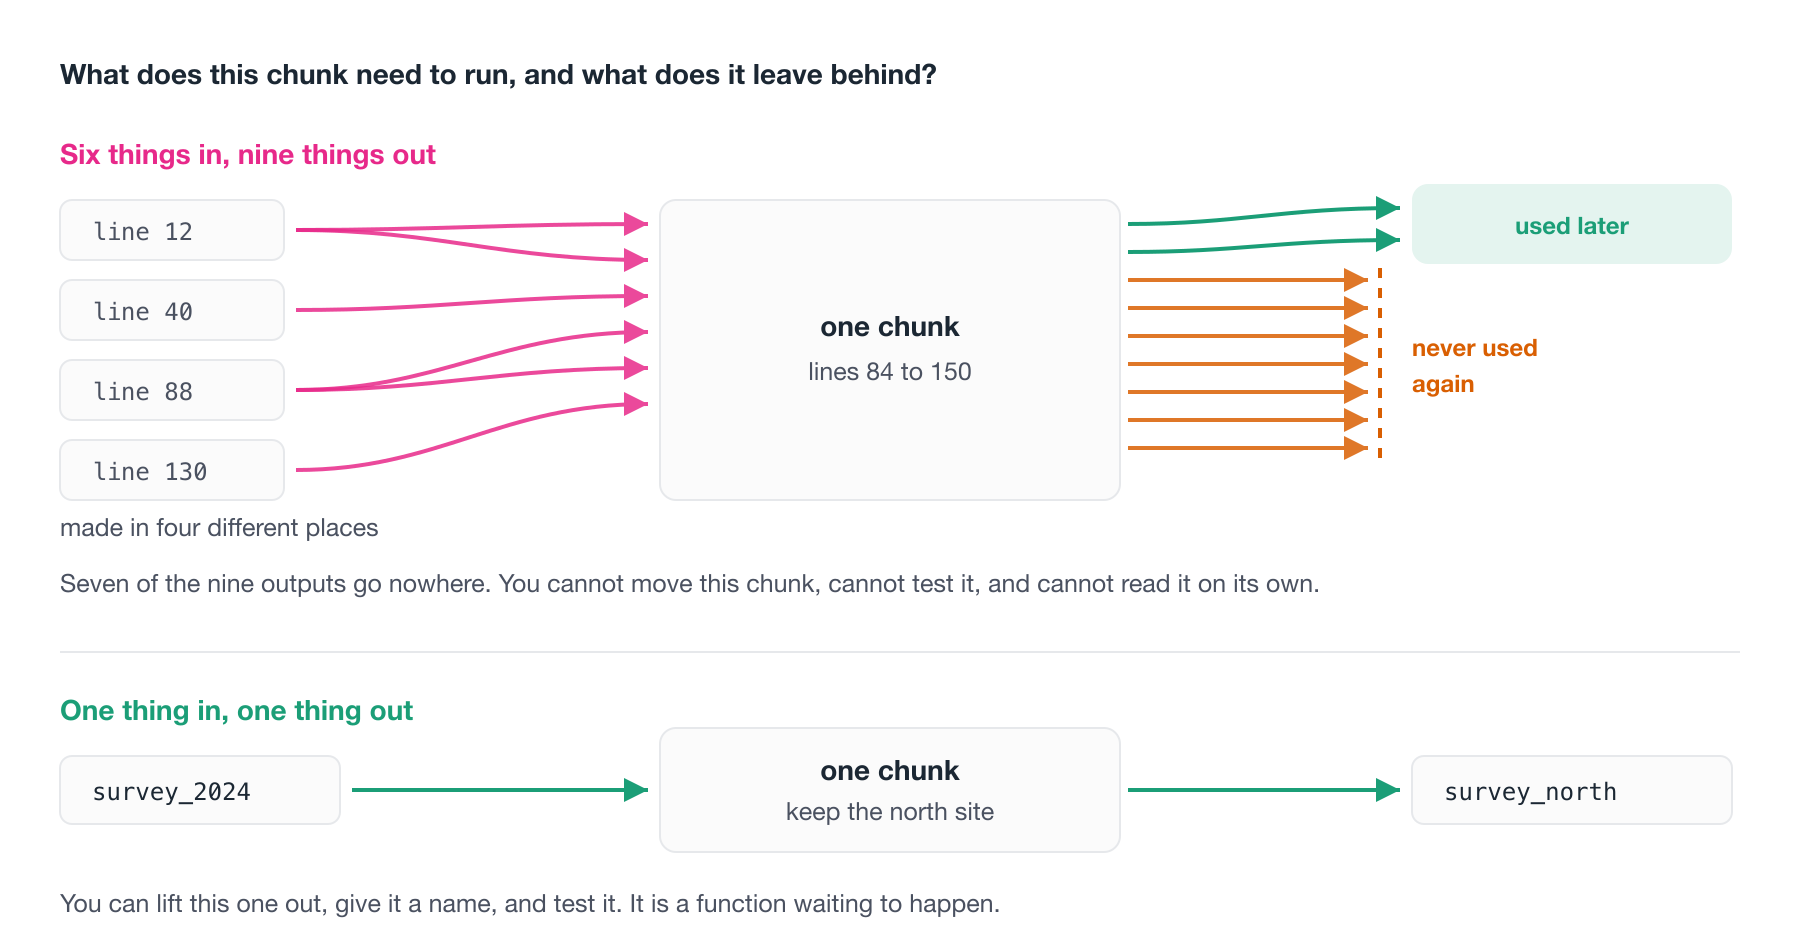
\includegraphics[width=1\linewidth,height=\textheight,keepaspectratio,alt={Two chunks compared. The first is fed by six pink arrows leaving four boxes labelled line 12, line 40, line 88 and line 130, and emits nine arrows: two green ones reach a box marked used later, and seven orange ones stop dead at a dashed wall marked never used again. The second chunk takes one green arrow in from survey\_2024 and sends one green arrow out to survey\_north.}]{figs/chunk-inputs-outputs.png}

}

\caption{Count the arrows going in and the arrows coming out. That count
is the finding.}

\end{figure}%

\subsection{Complexity that has a simpler
form}\label{complexity-that-has-a-simpler-form}

Sometimes code is doing something perfectly reasonable in a roundabout
way, and R already has the direct version.

\begin{Shaded}
\begin{Highlighting}[]
\FunctionTok{sapply}\NormalTok{(my\_list, }\ControlFlowTok{function}\NormalTok{(i) }\FunctionTok{length}\NormalTok{(i))}
\end{Highlighting}
\end{Shaded}

That works, but R already has:

\begin{Shaded}
\begin{Highlighting}[]
\FunctionTok{lengths}\NormalTok{(my\_list)}
\end{Highlighting}
\end{Shaded}

Same answer, and now the line says what it means rather than how it is
done.

You cannot spot these unless you happen to know the shortcut, which is a
bit unfair. So do not go hunting for them. Just notice when a line feels
like more machinery than the idea deserves, and have a look.

\subsection{Refactoring}\label{refactoring}

\textbf{Refactoring} means changing code while keeping its behaviour the
same.

It is like giving a car a service, or replacing parts that have worn
out. The car still drives the same, it just does so more reliably.

This is the move you make once you have found a smell. The behaviour is
fine, and the expression of it is not.

\section{A process for reviewing
code}\label{a-process-for-reviewing-code}

Here is the process I actually use, and it works on my own code as well
as on other people's.

The principle underneath it is this: \textbf{let the machine review the
mechanics, so that people can review the thinking.}

If a human reviewer spends their attention on spacing, on a misspelled
word in a comment, or on \texttt{any(is.na(x))}, that attention is gone
and it was worth almost nothing. Those are all things a tool does
perfectly, instantly, every time.

\begin{figure}[ht]

{\centering 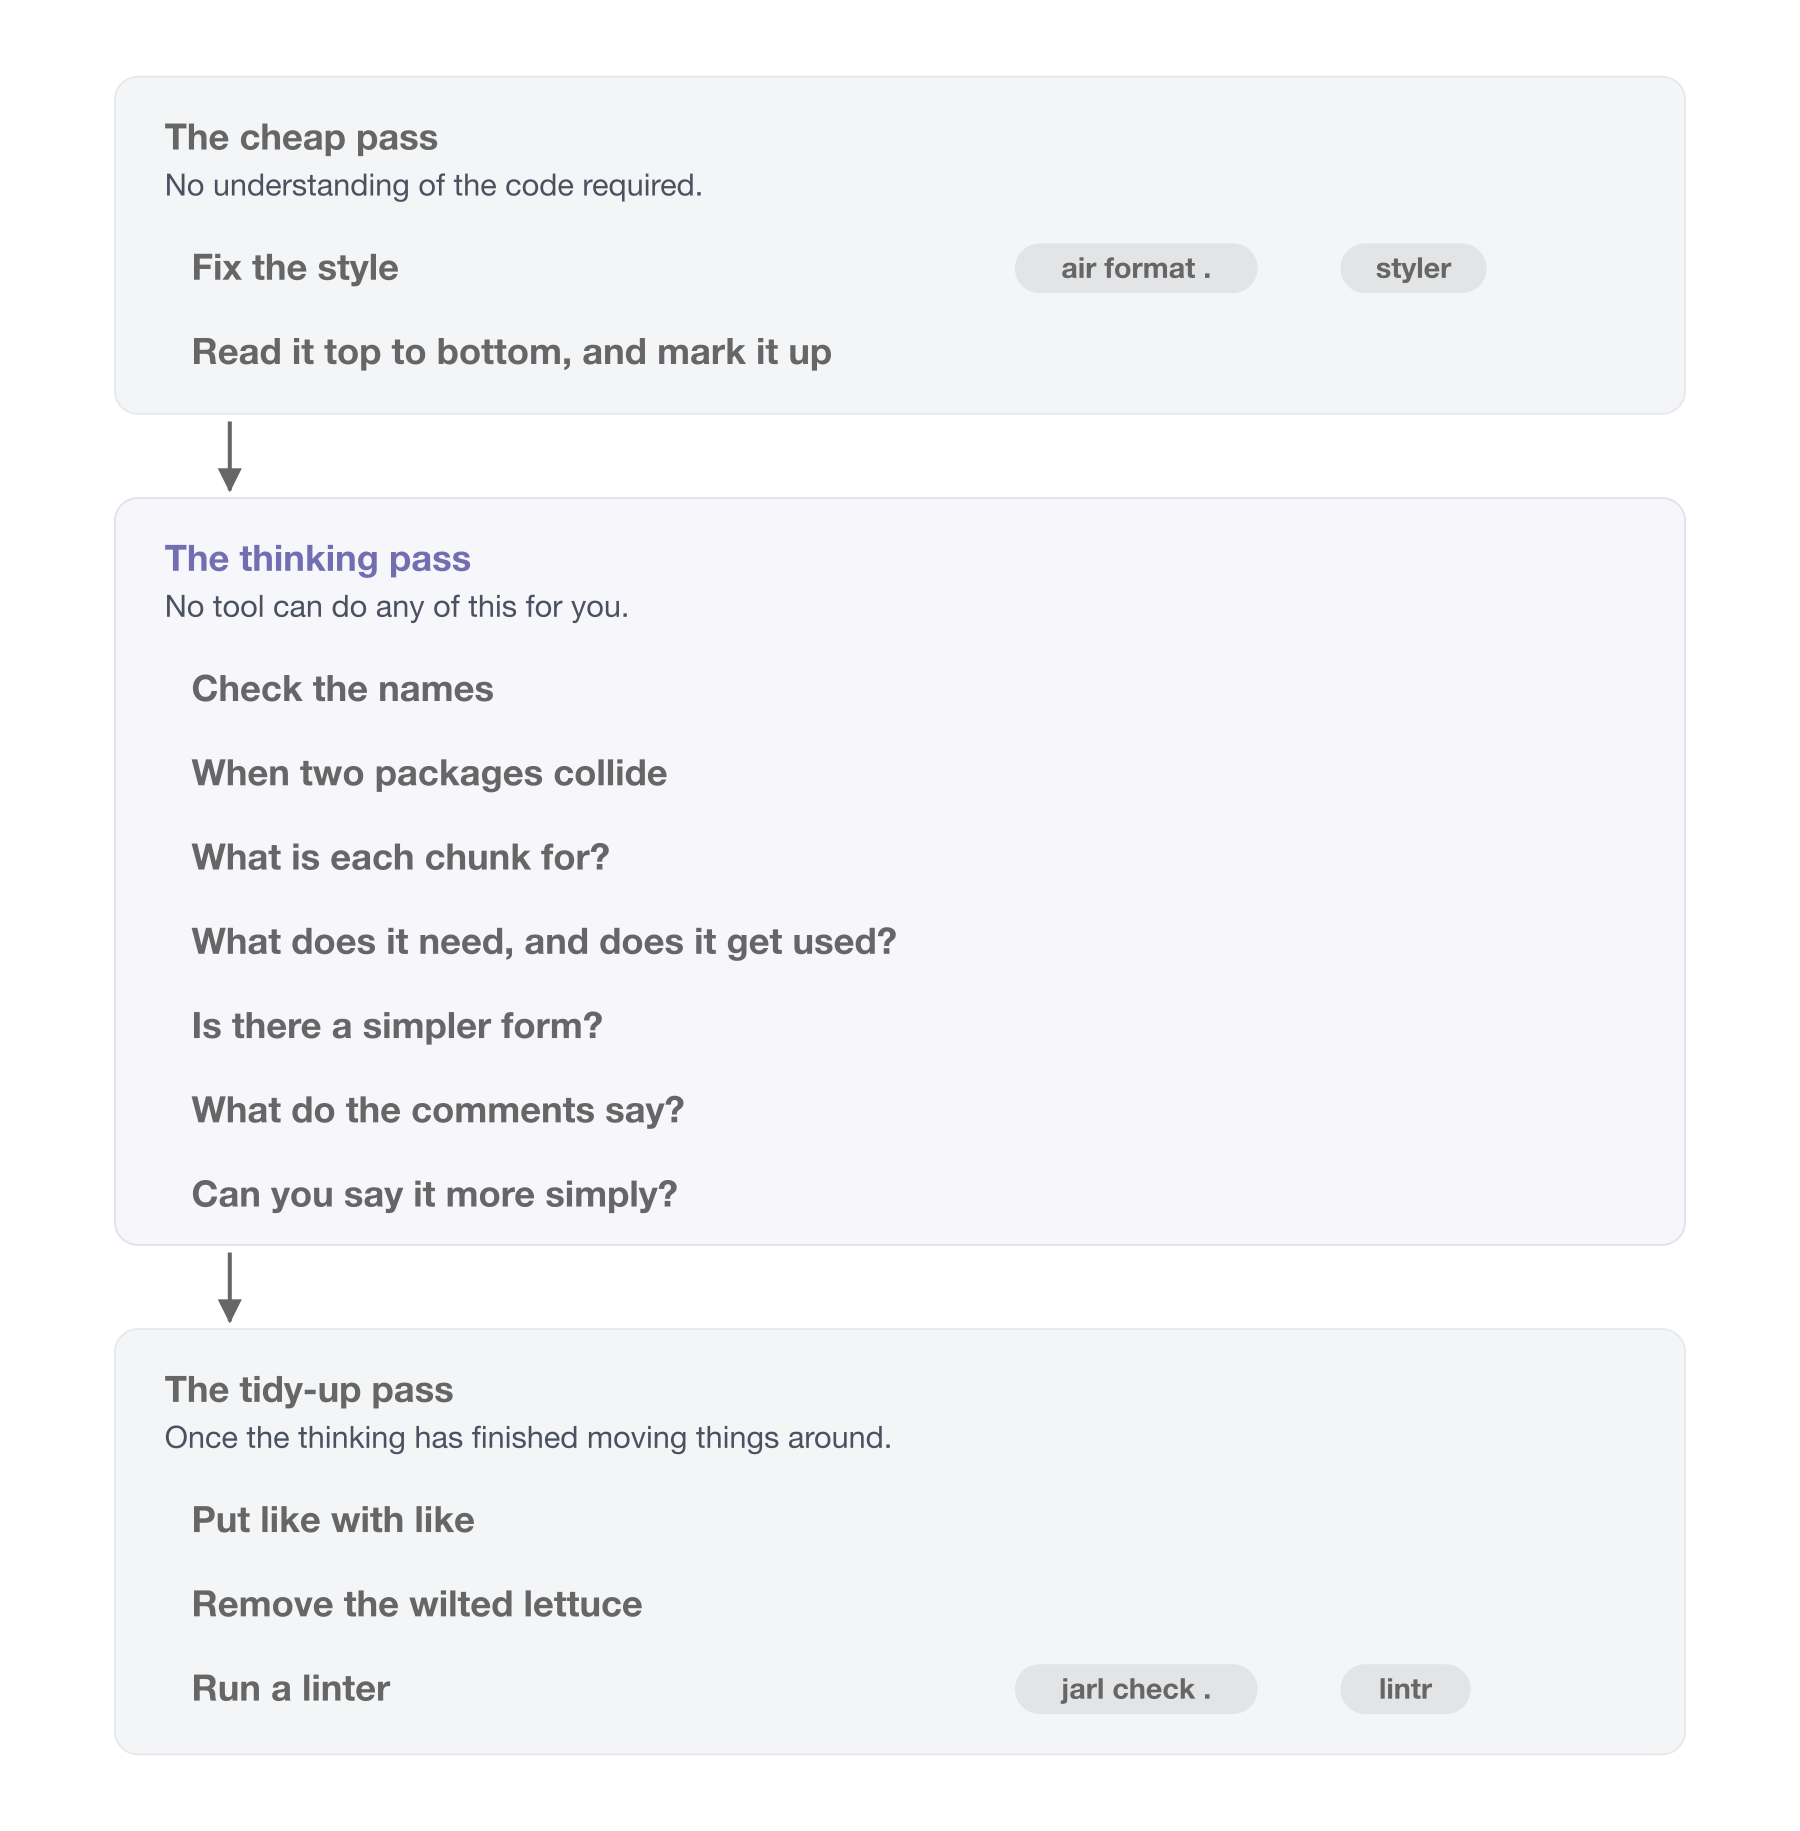
\includegraphics[width=1\linewidth,height=\textheight,keepaspectratio,alt={Two stacked bands. The upper grey band holds step 1, run the automated checks first, with pills for air format, jarl check, spelling colon colon spell underscore check underscore files, and restart R run from the top; it is labelled done by a machine, in seconds. An arrow crosses the gap saying only then is it worth a person\textquotesingle s time. The lower purple band holds steps 2 to 5 --- read it top to bottom and edit nothing, chunk it up, expression, and re-expression --- labelled only a person can do these.}]{figs/review-process-machine-then-person.png}

}

\caption{One of these five steps is a machine's job. The other four are
the review.}

\end{figure}%

\subsection{1. Run the automated checks
first}\label{run-the-automated-checks-first}

Before anyone reads it:

\begin{itemize}
\tightlist
\item
  \textbf{Format it.} \texttt{air\ format\ .}
\item
  \textbf{Lint it.} \texttt{jarl\ check\ .} or
  \texttt{lintr::lint\_dir()}
\item
  \textbf{Spell check it.} \texttt{spelling::spell\_check\_files()}
\item
  \textbf{Check the package habits.} \texttt{goodpractice::gp()}, if
  it's a package
\item
  \textbf{Run it from a clean session.} Restart R, run from the top. If
  it doesn't run, nothing else matters yet.
\end{itemize}

Only then is it worth a person's time.

\subsection{2. Read it top to bottom, and don't edit
anything}\label{read-it-top-to-bottom-and-dont-edit-anything}

This one is harder than it sounds, because the urge to fix the first
thing you see is strong.

Resist it, because on this pass you are only getting the shape of the
thing.

What you are collecting is a list of the places where the code caught
you. The bits where it did not quite make sense, or where something was
not clear, or where you had to read a line twice.

Those moments are the data, so mark them and keep going.

\subsection{3. Chunk it up}\label{chunk-it-up}

Now put similar things together.

\begin{itemize}
\tightlist
\item
  All \texttt{library()} calls at the top, in alphabetical order.
\item
  All function definitions together.
\item
  If a variable is defined at line 10 and isn't used until line 150,
  move them closer to each other.
\item
  Sections of code that do similar things should sit near each other.
\item
  Add commented section headers so you can see where a new area starts.
\item
  If one of those sections gets long, should it be its own script?
\end{itemize}

None of this changes what the code does, and all of it changes how much
you have to hold in your head to read it.

\subsection{4. Expression: can you follow
it?}\label{expression-can-you-follow-it}

Now go back to the places that caught you in step 2.

For each one: \textbf{do you understand what the code is doing when you
read it?}

Not what it does line by line. What it's \emph{for}. If you can't say it
in a sentence, that's the finding.

\subsection{5. Re-expression: can you say it more
simply?}\label{re-expression-can-you-say-it-more-simply}

The last question is the useful one.

\textbf{Can you re-express the intention of the code, and keep the
output the same?}

That is refactoring, and it is where the smells you noticed earlier get
cashed in. The copied block becomes a function, the nine objects become
one, and the \texttt{sapply} becomes \texttt{lengths}.

Then you run it again and check that the output did not move.

\begin{tcolorbox}[enhanced jigsaw, arc=.35mm, bottomrule=.15mm, bottomtitle=1mm, breakable, colback=white, colbacktitle=quarto-callout-tip-color!10!white, colframe=quarto-callout-tip-color-frame, coltitle=black, left=2mm, leftrule=.75mm, opacityback=0, opacitybacktitle=0.6, rightrule=.15mm, title=\textcolor{quarto-callout-tip-color}{\faLightbulb}\hspace{0.5em}{Some questions worth asking as you go}, titlerule=0mm, toprule=.15mm, toptitle=1mm]

\textbf{Can I tell what this is for?} If you cannot say it in a
sentence, that is the finding.

\textbf{Is the running order obvious?} Could a stranger tell what to run
first?

\textbf{Are the names consistent, and do they mean anything?}
\texttt{get.data()} versus \texttt{getData()} versus
\texttt{get\_data()} in one project is a real cost, paid every time
someone has to remember which.

\textbf{Can I reason about each piece separately?} Or do I have to hold
the whole thing in my head at once? This is the chunking question from
earlier, asked about someone else's code.

\textbf{What would break if the data changed slightly?} Extra column, a
new \texttt{NA}, a factor level nobody expected.

\textbf{Is anything here that I could regenerate?} Or, conversely, is
anything precious sitting somewhere disposable?

\end{tcolorbox}

\begin{tcolorbox}[enhanced jigsaw, arc=.35mm, bottomrule=.15mm, bottomtitle=1mm, breakable, colback=white, colbacktitle=quarto-callout-note-color!10!white, colframe=quarto-callout-note-color-frame, coltitle=black, left=2mm, leftrule=.75mm, opacityback=0, opacitybacktitle=0.6, rightrule=.15mm, title=\textcolor{quarto-callout-note-color}{\faInfo}\hspace{0.5em}{Your Turn}, titlerule=0mm, toprule=.15mm, toptitle=1mm]

\begin{enumerate}
\def\labelenumi{\arabic{enumi}.}
\tightlist
\item
  Run steps 1 to 3 on \texttt{07-needs-review/analysis.R}. Actually run
  \texttt{air} and the linter. Don't just read them.
\item
  The code still isn't easy to follow. Write down three places where it
  caught you.
\item
  Pick one and do step 5. Re-express it, then check the output hasn't
  changed.
\end{enumerate}

\end{tcolorbox}

\section{Reviewing someone else's
code}\label{reviewing-someone-elses-code}

Everything above works on your own code. Doing it to someone else's is a
different skill, and most of the difference is social rather than
technical.

\subsection{Start by asking what they
want}\label{start-by-asking-what-they-want}

The most useful question you can ask before reading a single line is:
\textbf{what kind of feedback are you looking for?}

Someone who wants to know whether the statistics are right does not want
thirty comments about variable names.

And the second question: \textbf{what is this code meant to do?}

Find the intention before you review the implementation. Half of what
looks like a mistake turns out to be a decision you didn't have the
context for.

\subsection{Non-adversarial, on
purpose}\label{non-adversarial-on-purpose}

Review is not a verdict. The goal is better code, not a judgement about
whether the code passed.

That sounds obvious written down, and it is surprisingly easy to lose
once you are twenty comments deep.

Two things that keep it on track.

\textbf{Review the code, not the person.} ``This function is doing three
things'' is useful. ``You always overcomplicate things'' isn't.

\textbf{Say what's good, specifically.} This is not politeness. If you
only ever name problems, people learn what to avoid but never what to
aim for.

\subsection{Exercise the code, don't just read
it}\label{exercise-the-code-dont-just-read-it}

Don't review from reading alone. Run it.

Then run it on something slightly different from what the author ran it
on. Your data, an extra column, a year that isn't in their file.

Reading tells you whether code is comprehensible. Running it on
something unfamiliar is what surfaces the assumptions the author didn't
know they were making.

\subsection{It will be slow at first}\label{it-will-be-slow-at-first}

Your first few reviews will take ages, and you will finish them feeling
like you did not have much to say.

That is normal, and it is what reviewing is like at the start.

Reviewing is a skill like any other, and it gets faster with practice.
The people who seem to spot things instantly have simply read a lot of
code.

\begin{tcolorbox}[enhanced jigsaw, arc=.35mm, bottomrule=.15mm, bottomtitle=1mm, breakable, colback=white, colbacktitle=quarto-callout-tip-color!10!white, colframe=quarto-callout-tip-color-frame, coltitle=black, left=2mm, leftrule=.75mm, opacityback=0, opacitybacktitle=0.6, rightrule=.15mm, title=\textcolor{quarto-callout-tip-color}{\faLightbulb}\hspace{0.5em}{If you want to see this done at full scale}, titlerule=0mm, toprule=.15mm, toptitle=1mm]

Open software peer review is the most developed version of this
practice, and it is all public.
\href{https://devguide.ropensci.org/softwarereview_reviewer.html}{rOpenSci's
reviewer guide} sets out what a reviewer is asked to look at, and their
\href{https://devguide.ropensci.org/reviewtemplate.html}{review
template} is the checklist itself. Reviews happen in the open on GitHub
and are signed, so you can read hundreds of real ones.

Two things there are worth stealing even for a small analysis project:
reviews are explicitly \textbf{non-adversarial}, because the goal is
better software rather than a verdict. And reviewers are asked to
comment on things a checklist can't capture, such as whether the
argument names read well and autocomplete sensibly.

That last one should sound familiar from the naming lesson.

\end{tcolorbox}

\begin{tcolorbox}[enhanced jigsaw, arc=.35mm, bottomrule=.15mm, bottomtitle=1mm, breakable, colback=white, colbacktitle=quarto-callout-note-color!10!white, colframe=quarto-callout-note-color-frame, coltitle=black, left=2mm, leftrule=.75mm, opacityback=0, opacitybacktitle=0.6, rightrule=.15mm, title=\textcolor{quarto-callout-note-color}{\faInfo}\hspace{0.5em}{Your Turn}, titlerule=0mm, toprule=.15mm, toptitle=1mm]

\begin{enumerate}
\def\labelenumi{\arabic{enumi}.}
\tightlist
\item
  Pair up. Swap the version of \texttt{analysis.R} you tidied earlier.
\item
  Before you read it, ask your partner the two questions: what feedback
  do they want, and what is the code meant to do?
\item
  Give three pieces of feedback. At least one of them should be
  something that's working well.
\end{enumerate}

\end{tcolorbox}

\begin{tcolorbox}[enhanced jigsaw, arc=.35mm, bottomrule=.15mm, bottomtitle=1mm, breakable, colback=white, colbacktitle=quarto-callout-tip-color!10!white, colframe=quarto-callout-tip-color-frame, coltitle=black, left=2mm, leftrule=.75mm, opacityback=0, opacitybacktitle=0.6, rightrule=.15mm, title=\textcolor{quarto-callout-tip-color}{\faLightbulb}\hspace{0.5em}{If you want a harder one: real code, real stranger}, titlerule=0mm, toprule=.15mm, toptitle=1mm]

Everything you've reviewed so far was written for this course.
\texttt{08-real-code-from-the-wild/} in the messy project repo wasn't.
It's a published survey script from the US Fish and Wildlife Service,
used here because it's released under CC0, and it is messy in ways
nobody planned.

The exercise is the same one you just did, with one part removed: you
cannot ask the author either of the two questions. You have the code, a
README, and nothing else.

That is the more common situation. Most code you inherit comes from
someone who has left, moved teams, or simply doesn't remember. Notice
what you end up doing instead of asking --- and notice how much of the
intention you can recover from the code itself, which is the best
argument there is for writing readable code in the first place.

Run \texttt{air} and the linter first, as before. Both find something.
Neither finds the thing that matters.

\end{tcolorbox}

\section{Clean as you go}\label{clean-as-you-go}

Get into the habit of going back over your code briefly to tidy it up,
as you go.

A kitchen analogy is useful here. Professional kitchens clean as they
go, because a tidy workspace keeps your mind clear and because the
alternative is an unusable bench by service. The same is true of code.

I rarely write my best code on the first pass. It gets better with
iteration.

So iterate briefly, as you go:

\begin{itemize}
\tightlist
\item
  Clean up the random comments that no longer mean anything.
\item
  Remove the wilted lettuce. These are the commented-out chunks of code
  you \emph{might just come back to}. You probably won't. If one really
  is important, write a comment explaining why it might be relevant,
  rather than leaving it lying there.
\item
  Fix the style.
\item
  Check the names.
\item
  Consider tidying up the implementation, refactoring it.
\end{itemize}

You might not have time to do all of these, or to do them thoroughly.
Doing \emph{some} of them will still leave you with better code, and you
get better at doing them the more you practise.

\begin{tcolorbox}[enhanced jigsaw, arc=.35mm, bottomrule=.15mm, bottomtitle=1mm, breakable, colback=white, colbacktitle=quarto-callout-tip-color!10!white, colframe=quarto-callout-tip-color-frame, coltitle=black, left=2mm, leftrule=.75mm, opacityback=0, opacitybacktitle=0.6, rightrule=.15mm, title=\textcolor{quarto-callout-tip-color}{\faLightbulb}\hspace{0.5em}{If we can see your code, we can trust it}, titlerule=0mm, toprule=.15mm, toptitle=1mm]

Version control isn't part of this course. It has its own.

But it's worth saying plainly that the single biggest improvement to
reviewability is putting your code somewhere it can be seen, with a
history.

Review is much easier when the reviewer can see not just what the code
is, but how it got that way.

\end{tcolorbox}

\begin{tcolorbox}[enhanced jigsaw, arc=.35mm, bottomrule=.15mm, bottomtitle=1mm, breakable, colback=white, colbacktitle=quarto-callout-note-color!10!white, colframe=quarto-callout-note-color-frame, coltitle=black, left=2mm, leftrule=.75mm, opacityback=0, opacitybacktitle=0.6, rightrule=.15mm, title=\textcolor{quarto-callout-note-color}{\faInfo}\hspace{0.5em}{Your Turn}, titlerule=0mm, toprule=.15mm, toptitle=1mm]

\begin{enumerate}
\def\labelenumi{\arabic{enumi}.}
\tightlist
\item
  Open a script of your own. One you wrote at least a month ago.
\item
  Give it ten minutes of clean-as-you-go. Comments, wilted lettuce,
  style, names.
\item
  Ten minutes only. What did you get done, and what would you do next?
\end{enumerate}

\end{tcolorbox}

\begin{tcolorbox}[enhanced jigsaw, arc=.35mm, bottomrule=.15mm, bottomtitle=1mm, breakable, colback=white, colbacktitle=quarto-callout-tip-color!10!white, colframe=quarto-callout-tip-color-frame, coltitle=black, left=2mm, leftrule=.75mm, opacityback=0, opacitybacktitle=0.6, rightrule=.15mm, title=\textcolor{quarto-callout-tip-color}{\faLightbulb}\hspace{0.5em}{Read more}, titlerule=0mm, toprule=.15mm, toptitle=1mm]

Parts of this chapter are adapted from my blog post,
\href{https://www.njtierney.com/posts/2023-10-30-how-to-get-good-with-r/}{How
to get good with R}.

\end{tcolorbox}

\bookmarksetup{startatroot}

\chapter{Writing functions}\label{writing-functions-1}

At some point you notice you have copied the same six lines for the
third time, with one number changed each time. That is a function
waiting to happen.

This section is about noticing that moment, and knowing what to do about
it. We look at the problem functions solve, what a good small function
looks like, and how to get inside one when it misbehaves.

\section{Overview}\label{overview-3}

\begin{itemize}
\tightlist
\item
  \textbf{Duration} 60 minutes
\end{itemize}

\section{Questions}\label{questions-3}

\begin{itemize}
\tightlist
\item
  What problem do functions actually solve?
\item
  What does a well-designed function look like?
\item
  How do I look inside a function when it goes wrong?
\end{itemize}

\section{The problem functions solve}\label{the-problem-functions-solve}

I do not think I can overstate this: learning to write functions changed
how I think about code, and how I think about solving problems. It takes
time to develop, and the payoff is enormous.

Let me tell you how I got there, because I got there slowly.

In 2013 I was writing code to calculate a t-test from scratch. At the
top of my script was something like:

\begin{Shaded}
\begin{Highlighting}[]
\NormalTok{var\_1 }\OtherTok{\textless{}{-}}\NormalTok{ data}\SpecialCharTok{$}\NormalTok{x1}
\NormalTok{var\_2 }\OtherTok{\textless{}{-}}\NormalTok{ data}\SpecialCharTok{$}\NormalTok{x2}
\end{Highlighting}
\end{Shaded}

and then a pile of code that computed the result.

\begin{tcolorbox}[enhanced jigsaw, arc=.35mm, bottomrule=.15mm, bottomtitle=1mm, breakable, colback=white, colbacktitle=quarto-callout-tip-color!10!white, colframe=quarto-callout-tip-color-frame, coltitle=black, left=2mm, leftrule=.75mm, opacityback=0, opacitybacktitle=0.6, rightrule=.15mm, title=\textcolor{quarto-callout-tip-color}{\faLightbulb}\hspace{0.5em}{The whole script, if you want to see it}, titlerule=0mm, toprule=.15mm, toptitle=1mm]

This is roughly what the rest of it looked like. You do not need to read
it closely. The thing I want you to notice is how much of it there is,
and where the two lines I kept editing are.

\protect\phantomsection\label{annotated-cell-117}%
\begin{Shaded}
\begin{Highlighting}[]
\NormalTok{var\_1 }\OtherTok{\textless{}{-}}\NormalTok{ data}\SpecialCharTok{$}\NormalTok{x1 }\hspace*{\fill}\NormalTok{\circled{1}}
\NormalTok{var\_2 }\OtherTok{\textless{}{-}}\NormalTok{ data}\SpecialCharTok{$}\NormalTok{x2 }

\NormalTok{n\_1 }\OtherTok{\textless{}{-}} \FunctionTok{length}\NormalTok{(var\_1)}
\NormalTok{n\_2 }\OtherTok{\textless{}{-}} \FunctionTok{length}\NormalTok{(var\_2)}

\NormalTok{mean\_1 }\OtherTok{\textless{}{-}} \FunctionTok{mean}\NormalTok{(var\_1)}
\NormalTok{mean\_2 }\OtherTok{\textless{}{-}} \FunctionTok{mean}\NormalTok{(var\_2)}

\NormalTok{var\_within\_1 }\OtherTok{\textless{}{-}} \FunctionTok{sum}\NormalTok{((var\_1 }\SpecialCharTok{{-}}\NormalTok{ mean\_1)}\SpecialCharTok{\^{}}\DecValTok{2}\NormalTok{) }\SpecialCharTok{/}\NormalTok{ (n\_1 }\SpecialCharTok{{-}} \DecValTok{1}\NormalTok{)}
\NormalTok{var\_within\_2 }\OtherTok{\textless{}{-}} \FunctionTok{sum}\NormalTok{((var\_2 }\SpecialCharTok{{-}}\NormalTok{ mean\_2)}\SpecialCharTok{\^{}}\DecValTok{2}\NormalTok{) }\SpecialCharTok{/}\NormalTok{ (n\_2 }\SpecialCharTok{{-}} \DecValTok{1}\NormalTok{)}

\NormalTok{pooled\_var }\OtherTok{\textless{}{-}}\NormalTok{ ((n\_1 }\SpecialCharTok{{-}} \DecValTok{1}\NormalTok{) }\SpecialCharTok{*}\NormalTok{ var\_within\_1 }\SpecialCharTok{+}\NormalTok{ (n\_2 }\SpecialCharTok{{-}} \DecValTok{1}\NormalTok{) }\SpecialCharTok{*}\NormalTok{ var\_within\_2) }\SpecialCharTok{/}\NormalTok{ (n\_1 }\SpecialCharTok{+}\NormalTok{ n\_2 }\SpecialCharTok{{-}} \DecValTok{2}\NormalTok{)}
\NormalTok{std\_error }\OtherTok{\textless{}{-}} \FunctionTok{sqrt}\NormalTok{(pooled\_var }\SpecialCharTok{*}\NormalTok{ (}\DecValTok{1} \SpecialCharTok{/}\NormalTok{ n\_1 }\SpecialCharTok{+} \DecValTok{1} \SpecialCharTok{/}\NormalTok{ n\_2))}

\NormalTok{t\_statistic }\OtherTok{\textless{}{-}}\NormalTok{ (mean\_1 }\SpecialCharTok{{-}}\NormalTok{ mean\_2) }\SpecialCharTok{/}\NormalTok{ std\_error}
\NormalTok{degrees\_freedom }\OtherTok{\textless{}{-}}\NormalTok{ n\_1 }\SpecialCharTok{+}\NormalTok{ n\_2 }\SpecialCharTok{{-}} \DecValTok{2}
\NormalTok{p\_value }\OtherTok{\textless{}{-}} \DecValTok{2} \SpecialCharTok{*} \FunctionTok{pt}\NormalTok{(}\SpecialCharTok{{-}}\FunctionTok{abs}\NormalTok{(t\_statistic), }\AttributeTok{df =}\NormalTok{ degrees\_freedom)}

\NormalTok{t\_statistic}
\NormalTok{p\_value}
\end{Highlighting}
\end{Shaded}

\begin{description}
\tightlist
\item[\circled{1}]
These two lines are the only part that ever changed.
\end{description}

\end{tcolorbox}

Every time I wanted to look at a different pair of variables, I went
back to the top, changed those two lines, and ran the whole script
again.

Two lines out of twenty. The other eighteen never changed, and I re-ran
all of them, by hand, every single time.

Something about this felt wrong. But I didn't have the words for it.

What I was reaching for sounded something like:

\begin{quote}
I want to run this script, but get the top couple of lines to change
depending on which variables I specify.
\end{quote}

What I needed was a function. I just didn't know it.

I had been \emph{taught} functions by then. And I had been \emph{using}
functions the whole time, things like \texttt{lm()}, \texttt{table()},
\texttt{subset()}, and \texttt{read.csv()}. I used them every day
without ever thinking about where they came from, or that I could make
my own.

But the examples I was taught with were ``convert Celsius to
Fahrenheit'' and ``identify odd numbers'', and I couldn't see how those
applied to anything I actually did.

They seemed like useful kitchen trinkets. An apple corer, a garlic
press. Rather than a fundamental skill, like knowing how to use a knife.

Functions are the knife.

So rather than argue that, let me show you.

What does this code do?

\begin{Shaded}
\begin{Highlighting}[]
\NormalTok{dat }\OtherTok{\textless{}{-}}\NormalTok{ tibble}\SpecialCharTok{::}\FunctionTok{tibble}\NormalTok{(}
  \AttributeTok{weight =} \FunctionTok{rnorm}\NormalTok{(}\DecValTok{10}\NormalTok{, }\AttributeTok{mean =} \DecValTok{80}\NormalTok{, }\AttributeTok{sd =} \DecValTok{6}\NormalTok{),}
  \AttributeTok{height =} \FunctionTok{rnorm}\NormalTok{(}\DecValTok{10}\NormalTok{, }\AttributeTok{mean =} \DecValTok{165}\NormalTok{, }\AttributeTok{sd =} \DecValTok{10}\NormalTok{)}
\NormalTok{)}

\NormalTok{dat}\SpecialCharTok{$}\NormalTok{weight\_0 }\OtherTok{\textless{}{-}}\NormalTok{ (dat}\SpecialCharTok{$}\NormalTok{weight }\SpecialCharTok{{-}} \FunctionTok{mean}\NormalTok{(dat}\SpecialCharTok{$}\NormalTok{weight, }\AttributeTok{na.rm =} \ConstantTok{TRUE}\NormalTok{)) }\SpecialCharTok{/} \FunctionTok{sd}\NormalTok{(dat}\SpecialCharTok{$}\NormalTok{weight, }\AttributeTok{na.rm =} \ConstantTok{TRUE}\NormalTok{)}

\NormalTok{dat}\SpecialCharTok{$}\NormalTok{height\_0 }\OtherTok{\textless{}{-}}\NormalTok{ (dat}\SpecialCharTok{$}\NormalTok{height }\SpecialCharTok{{-}} \FunctionTok{mean}\NormalTok{(dat}\SpecialCharTok{$}\NormalTok{height, }\AttributeTok{na.rm =} \ConstantTok{TRUE}\NormalTok{)) }\SpecialCharTok{/} \FunctionTok{sd}\NormalTok{(dat}\SpecialCharTok{$}\NormalTok{weight, }\AttributeTok{na.rm =} \ConstantTok{TRUE}\NormalTok{)}
\end{Highlighting}
\end{Shaded}

Before you read on, have a proper go at this one. It is the whole
argument of this chapter in a single example.

\begin{tcolorbox}[enhanced jigsaw, arc=.35mm, bottomrule=.15mm, bottomtitle=1mm, breakable, colback=white, colbacktitle=quarto-callout-note-color!10!white, colframe=quarto-callout-note-color-frame, coltitle=black, left=2mm, leftrule=.75mm, opacityback=0, opacitybacktitle=0.6, rightrule=.15mm, title=\textcolor{quarto-callout-note-color}{\faInfo}\hspace{0.5em}{Your Turn}, titlerule=0mm, toprule=.15mm, toptitle=1mm]

Look at those two lines of code. Don't run them.

\begin{enumerate}
\def\labelenumi{\arabic{enumi}.}
\tightlist
\item
  In one sentence, what is this code doing?
\item
  There is a bug in it. Find it.
\item
  How long did that take you, and what made it hard?
\end{enumerate}

\end{tcolorbox}

So, what is it doing?

This is mean centering and scaling. It's a transformation that gives
your data a mean of 0 and a standard deviation of 1, which some
statistical models want.

But reading that code, it's hard to see that's what's happening. Nothing
in it says ``centre and scale''. You have to reconstruct the intent from
the arithmetic.

Worse, it invites errors, because you have to repeat
\texttt{dat\$weight} or \texttt{dat\$height} several times per line.

And there \emph{is} an error.

Look at the second line again. For \texttt{height\_0}, I divide by the
standard deviation of \textbf{weight}, not height.

That's a copy-paste bug, it's completely silent, and it produces numbers
that look entirely plausible. If you found it, well done. If you didn't,
that is exactly the point, and it is why I would rather not rely on
either of us spotting it.

A function fixes this by \emph{abstracting away} the need to write the
variable in each time. Break it into two steps:

\begin{Shaded}
\begin{Highlighting}[]
\NormalTok{mean\_center }\OtherTok{\textless{}{-}} \ControlFlowTok{function}\NormalTok{(variable) \{}
\NormalTok{  variable }\SpecialCharTok{{-}} \FunctionTok{mean}\NormalTok{(variable, }\AttributeTok{na.rm =} \ConstantTok{TRUE}\NormalTok{)}
\NormalTok{\}}

\NormalTok{scale\_sd }\OtherTok{\textless{}{-}} \ControlFlowTok{function}\NormalTok{(variable) \{}
\NormalTok{  variable }\SpecialCharTok{/} \FunctionTok{sd}\NormalTok{(variable, }\AttributeTok{na.rm =} \ConstantTok{TRUE}\NormalTok{)}
\NormalTok{\}}
\end{Highlighting}
\end{Shaded}

Now we can write:

\begin{Shaded}
\begin{Highlighting}[]
\NormalTok{dat}\SpecialCharTok{$}\NormalTok{height }\SpecialCharTok{|\textgreater{}}
  \FunctionTok{mean\_center}\NormalTok{() }\SpecialCharTok{|\textgreater{}}
  \FunctionTok{scale\_sd}\NormalTok{()}
\end{Highlighting}
\end{Shaded}

Or write one function that does both steps:

\begin{Shaded}
\begin{Highlighting}[]
\NormalTok{center\_scale }\OtherTok{\textless{}{-}} \ControlFlowTok{function}\NormalTok{(variable) \{}
\NormalTok{  centered }\OtherTok{\textless{}{-}} \FunctionTok{mean\_center}\NormalTok{(variable)}
\NormalTok{  centered\_scaled }\OtherTok{\textless{}{-}} \FunctionTok{scale\_sd}\NormalTok{(centered)}
\NormalTok{  centered\_scaled}
\NormalTok{\}}
\end{Highlighting}
\end{Shaded}

What is nice here is that each function \emph{describes what it does} in
its name. Reading \texttt{center\_scale}, you can see it does a thing
called \texttt{mean\_center} first, then \texttt{scale\_sd} next.

So compare the original:

\begin{Shaded}
\begin{Highlighting}[]
\NormalTok{dat}\SpecialCharTok{$}\NormalTok{weight\_0 }\OtherTok{\textless{}{-}}\NormalTok{ (dat}\SpecialCharTok{$}\NormalTok{weight }\SpecialCharTok{{-}} \FunctionTok{mean}\NormalTok{(dat}\SpecialCharTok{$}\NormalTok{weight, }\AttributeTok{na.rm =} \ConstantTok{TRUE}\NormalTok{)) }\SpecialCharTok{/} \FunctionTok{sd}\NormalTok{(dat}\SpecialCharTok{$}\NormalTok{weight, }\AttributeTok{na.rm =} \ConstantTok{TRUE}\NormalTok{)}
\NormalTok{dat}\SpecialCharTok{$}\NormalTok{height\_0 }\OtherTok{\textless{}{-}}\NormalTok{ (dat}\SpecialCharTok{$}\NormalTok{height }\SpecialCharTok{{-}} \FunctionTok{mean}\NormalTok{(dat}\SpecialCharTok{$}\NormalTok{height, }\AttributeTok{na.rm =} \ConstantTok{TRUE}\NormalTok{)) }\SpecialCharTok{/} \FunctionTok{sd}\NormalTok{(dat}\SpecialCharTok{$}\NormalTok{weight, }\AttributeTok{na.rm =} \ConstantTok{TRUE}\NormalTok{)}
\end{Highlighting}
\end{Shaded}

with:

\begin{Shaded}
\begin{Highlighting}[]
\NormalTok{dat}\SpecialCharTok{$}\NormalTok{weight\_0 }\OtherTok{\textless{}{-}} \FunctionTok{center\_scale}\NormalTok{(dat}\SpecialCharTok{$}\NormalTok{weight)}
\NormalTok{dat}\SpecialCharTok{$}\NormalTok{height\_0 }\OtherTok{\textless{}{-}} \FunctionTok{center\_scale}\NormalTok{(dat}\SpecialCharTok{$}\NormalTok{height)}
\end{Highlighting}
\end{Shaded}

The bug I planted above isn't just fixed in the second version. It's
become almost impossible to write.

\begin{tcolorbox}[enhanced jigsaw, arc=.35mm, bottomrule=.15mm, bottomtitle=1mm, breakable, colback=white, colbacktitle=quarto-callout-tip-color!10!white, colframe=quarto-callout-tip-color-frame, coltitle=black, left=2mm, leftrule=.75mm, opacityback=0, opacitybacktitle=0.6, rightrule=.15mm, title=\textcolor{quarto-callout-tip-color}{\faLightbulb}\hspace{0.5em}{Someone has probably done this already}, titlerule=0mm, toprule=.15mm, toptitle=1mm]

Base R has \texttt{scale()}, which does exactly this, though it returns
a matrix so you need to wrap it:

\begin{Shaded}
\begin{Highlighting}[]
\NormalTok{dat}\SpecialCharTok{$}\NormalTok{weight\_0 }\OtherTok{\textless{}{-}} \FunctionTok{as.numeric}\NormalTok{(}\FunctionTok{scale}\NormalTok{(dat}\SpecialCharTok{$}\NormalTok{weight))}
\end{Highlighting}
\end{Shaded}

Which is a good argument for checking whether a solution exists before
writing your own. You don't need to write everything from scratch.

At worst you find nobody has solved your problem, which is an
opportunity. Usually you learn the words other people use to describe
it, which makes your next search much better.

\end{tcolorbox}

\subsection{Other things worth turning into a
function}\label{other-things-worth-turning-into-a-function}

Centering and scaling is one kind of job. Here are a few others, so the
idea doesn't get stuck to that one example.

\textbf{A calculation you keep redoing.} Body mass index, a rate per
thousand, a unit conversion.

\begin{Shaded}
\begin{Highlighting}[]
\NormalTok{bmi }\OtherTok{\textless{}{-}} \ControlFlowTok{function}\NormalTok{(weight\_kg, height\_m) \{}
\NormalTok{  weight\_kg }\SpecialCharTok{/}\NormalTok{ height\_m}\SpecialCharTok{\^{}}\DecValTok{2}
\NormalTok{\}}
\end{Highlighting}
\end{Shaded}

\textbf{A filter you keep re-typing, where the name is the useful part.}

\begin{Shaded}
\begin{Highlighting}[]
\NormalTok{adults\_only }\OtherTok{\textless{}{-}} \ControlFlowTok{function}\NormalTok{(data) \{}
\NormalTok{  data[data}\SpecialCharTok{$}\NormalTok{age }\SpecialCharTok{\textgreater{}=} \DecValTok{18}\NormalTok{, ]}
\NormalTok{\}}
\end{Highlighting}
\end{Shaded}

You could write that condition inline every time. But
\texttt{adults\_only(survey)} says what you meant, and the next reader
doesn't have to work out whether \texttt{\textgreater{}=\ 18} was
deliberate.

\textbf{A plot you make over and over with the same styling.}

\begin{Shaded}
\begin{Highlighting}[]
\NormalTok{plot\_by\_species }\OtherTok{\textless{}{-}} \ControlFlowTok{function}\NormalTok{(data, yvar) \{}
  \FunctionTok{ggplot}\NormalTok{(data, }\FunctionTok{aes}\NormalTok{(}\AttributeTok{x =}\NormalTok{ species, }\AttributeTok{y =}\NormalTok{ \{\{ yvar \}\})) }\SpecialCharTok{+}
    \FunctionTok{geom\_boxplot}\NormalTok{() }\SpecialCharTok{+}
    \FunctionTok{theme\_minimal}\NormalTok{()}
\NormalTok{\}}
\end{Highlighting}
\end{Shaded}

\textbf{A check you want to run on every dataset that comes in.}

\begin{Shaded}
\begin{Highlighting}[]
\NormalTok{n\_missing }\OtherTok{\textless{}{-}} \ControlFlowTok{function}\NormalTok{(data) \{}
  \FunctionTok{colSums}\NormalTok{(}\FunctionTok{is.na}\NormalTok{(data))}
\NormalTok{\}}
\end{Highlighting}
\end{Shaded}

None of these are clever. That is deliberate. Most of the functions I
write are three lines long and do something faintly boring, and they are
still the thing that makes the analysis readable.

\begin{tcolorbox}[enhanced jigsaw, arc=.35mm, bottomrule=.15mm, bottomtitle=1mm, breakable, colback=white, colbacktitle=quarto-callout-tip-color!10!white, colframe=quarto-callout-tip-color-frame, coltitle=black, left=2mm, leftrule=.75mm, opacityback=0, opacitybacktitle=0.6, rightrule=.15mm, title=\textcolor{quarto-callout-tip-color}{\faLightbulb}\hspace{0.5em}{Fifteen small functions worth having}, titlerule=0mm, toprule=.15mm, toptitle=1mm]

Here are fifteen I actually use, or something close to them. None is
more than a few lines. Read them for the \emph{shape} rather than the
detail, and steal any that look useful.

\textbf{Describing what you were given}

\begin{Shaded}
\begin{Highlighting}[]
\NormalTok{n\_missing }\OtherTok{\textless{}{-}} \ControlFlowTok{function}\NormalTok{(x) \{}
  \FunctionTok{sum}\NormalTok{(}\FunctionTok{is.na}\NormalTok{(x))}
\NormalTok{\}}

\NormalTok{n\_complete }\OtherTok{\textless{}{-}} \ControlFlowTok{function}\NormalTok{(x) \{}
  \FunctionTok{sum}\NormalTok{(}\SpecialCharTok{!}\FunctionTok{is.na}\NormalTok{(x))}
\NormalTok{\}}

\NormalTok{prop\_missing }\OtherTok{\textless{}{-}} \ControlFlowTok{function}\NormalTok{(x, }\AttributeTok{digits =} \DecValTok{2}\NormalTok{) \{}
  \FunctionTok{round}\NormalTok{(}\FunctionTok{n\_missing}\NormalTok{(x) }\SpecialCharTok{/} \FunctionTok{length}\NormalTok{(x), digits)}
\NormalTok{\}}

\NormalTok{missing\_by\_column }\OtherTok{\textless{}{-}} \ControlFlowTok{function}\NormalTok{(data) \{}
\NormalTok{  purrr}\SpecialCharTok{::}\FunctionTok{map\_int}\NormalTok{(data, n\_missing)}
\NormalTok{\}}

\NormalTok{count\_sorted }\OtherTok{\textless{}{-}} \ControlFlowTok{function}\NormalTok{(x) \{}
  \FunctionTok{sort}\NormalTok{(}\FunctionTok{table}\NormalTok{(x, }\AttributeTok{useNA =} \StringTok{"ifany"}\NormalTok{), }\AttributeTok{decreasing =} \ConstantTok{TRUE}\NormalTok{)}
\NormalTok{\}}
\end{Highlighting}
\end{Shaded}

\textbf{Summarising}

\begin{Shaded}
\begin{Highlighting}[]
\NormalTok{se }\OtherTok{\textless{}{-}} \ControlFlowTok{function}\NormalTok{(x, }\AttributeTok{na\_rm =} \ConstantTok{TRUE}\NormalTok{) \{}
  \FunctionTok{sd}\NormalTok{(x, }\AttributeTok{na.rm =}\NormalTok{ na\_rm) }\SpecialCharTok{/} \FunctionTok{sqrt}\NormalTok{(}\FunctionTok{n\_complete}\NormalTok{(x))}
\NormalTok{\}}

\NormalTok{ci\_95 }\OtherTok{\textless{}{-}} \ControlFlowTok{function}\NormalTok{(x) \{}
  \FunctionTok{mean}\NormalTok{(x, }\AttributeTok{na.rm =} \ConstantTok{TRUE}\NormalTok{) }\SpecialCharTok{+} \FunctionTok{c}\NormalTok{(}\SpecialCharTok{{-}}\FloatTok{1.96}\NormalTok{, }\FloatTok{1.96}\NormalTok{) }\SpecialCharTok{*} \FunctionTok{se}\NormalTok{(x)}
\NormalTok{\}}

\NormalTok{rate\_per\_1000 }\OtherTok{\textless{}{-}} \ControlFlowTok{function}\NormalTok{(events, population, }\AttributeTok{digits =} \DecValTok{1}\NormalTok{) \{}
  \FunctionTok{round}\NormalTok{(events }\SpecialCharTok{/}\NormalTok{ population }\SpecialCharTok{*} \DecValTok{1000}\NormalTok{, digits)}
\NormalTok{\}}
\end{Highlighting}
\end{Shaded}

\textbf{Cleaning}

\begin{Shaded}
\begin{Highlighting}[]
\NormalTok{recode\_missing }\OtherTok{\textless{}{-}} \ControlFlowTok{function}\NormalTok{(x, }\AttributeTok{values =} \FunctionTok{c}\NormalTok{(}\SpecialCharTok{{-}}\DecValTok{99}\NormalTok{, }\SpecialCharTok{{-}}\DecValTok{999}\NormalTok{, }\StringTok{""}\NormalTok{)) \{}
  \FunctionTok{ifelse}\NormalTok{(x }\SpecialCharTok{\%in\%}\NormalTok{ values, }\ConstantTok{NA}\NormalTok{, x)}
\NormalTok{\}}

\NormalTok{drop\_empty\_cols }\OtherTok{\textless{}{-}} \ControlFlowTok{function}\NormalTok{(data) \{}
\NormalTok{  keep }\OtherTok{\textless{}{-}}\NormalTok{ purrr}\SpecialCharTok{::}\FunctionTok{map\_int}\NormalTok{(data, n\_complete) }\SpecialCharTok{\textgreater{}} \DecValTok{0}
\NormalTok{  data[, keep, drop }\OtherTok{=} \ConstantTok{FALSE}\NormalTok{]}
\NormalTok{\}}

\NormalTok{complete\_rows }\OtherTok{\textless{}{-}} \ControlFlowTok{function}\NormalTok{(data) \{}
\NormalTok{  data[}\FunctionTok{complete.cases}\NormalTok{(data), ]}
\NormalTok{\}}
\end{Highlighting}
\end{Shaded}

\textbf{Checking, before you trust it}

\begin{Shaded}
\begin{Highlighting}[]
\NormalTok{check\_columns }\OtherTok{\textless{}{-}} \ControlFlowTok{function}\NormalTok{(data, required) \{}
\NormalTok{  missing\_cols }\OtherTok{\textless{}{-}} \FunctionTok{setdiff}\NormalTok{(required, }\FunctionTok{names}\NormalTok{(data))}
  \ControlFlowTok{if}\NormalTok{ (}\FunctionTok{length}\NormalTok{(missing\_cols) }\SpecialCharTok{\textgreater{}} \DecValTok{0}\NormalTok{) \{}
    \FunctionTok{stop}\NormalTok{(}\StringTok{"Missing columns: "}\NormalTok{, }\FunctionTok{paste}\NormalTok{(missing\_cols, }\AttributeTok{collapse =} \StringTok{", "}\NormalTok{))}
\NormalTok{  \}}
  \FunctionTok{invisible}\NormalTok{(data)}
\NormalTok{\}}

\NormalTok{is\_outlier }\OtherTok{\textless{}{-}} \ControlFlowTok{function}\NormalTok{(x, }\AttributeTok{mult =} \FloatTok{1.5}\NormalTok{) \{}
\NormalTok{  quartiles }\OtherTok{\textless{}{-}} \FunctionTok{quantile}\NormalTok{(x, }\FunctionTok{c}\NormalTok{(}\FloatTok{0.25}\NormalTok{, }\FloatTok{0.75}\NormalTok{), }\AttributeTok{na.rm =} \ConstantTok{TRUE}\NormalTok{)}
\NormalTok{  spread }\OtherTok{\textless{}{-}}\NormalTok{ quartiles[}\DecValTok{2}\NormalTok{] }\SpecialCharTok{{-}}\NormalTok{ quartiles[}\DecValTok{1}\NormalTok{]}
\NormalTok{  x }\SpecialCharTok{\textless{}}\NormalTok{ quartiles[}\DecValTok{1}\NormalTok{] }\SpecialCharTok{{-}}\NormalTok{ mult }\SpecialCharTok{*}\NormalTok{ spread }\SpecialCharTok{|}\NormalTok{ x }\SpecialCharTok{\textgreater{}}\NormalTok{ quartiles[}\DecValTok{2}\NormalTok{] }\SpecialCharTok{+}\NormalTok{ mult }\SpecialCharTok{*}\NormalTok{ spread}
\NormalTok{\}}
\end{Highlighting}
\end{Shaded}

\textbf{Looking at things}

\begin{Shaded}
\begin{Highlighting}[]
\NormalTok{head\_tail }\OtherTok{\textless{}{-}} \ControlFlowTok{function}\NormalTok{(data, }\AttributeTok{n =} \DecValTok{3}\NormalTok{) \{}
  \FunctionTok{rbind}\NormalTok{(}\FunctionTok{head}\NormalTok{(data, n), }\FunctionTok{tail}\NormalTok{(data, n))}
\NormalTok{\}}

\NormalTok{pct }\OtherTok{\textless{}{-}} \ControlFlowTok{function}\NormalTok{(prop, }\AttributeTok{digits =} \DecValTok{1}\NormalTok{) \{}
  \FunctionTok{paste0}\NormalTok{(}\FunctionTok{round}\NormalTok{(prop }\SpecialCharTok{*} \DecValTok{100}\NormalTok{, digits), }\StringTok{"\%"}\NormalTok{)}
\NormalTok{\}}
\end{Highlighting}
\end{Shaded}

Three things to notice across the whole list.

Several of them \textbf{call each other}. \texttt{prop\_missing()} uses
\texttt{n\_missing()}, \texttt{se()} uses \texttt{n\_complete()},
\texttt{ci\_95()} uses \texttt{se()}. None of them repeats the other's
logic.

Most of them are \textbf{named for the question they answer}, not for
how they answer it. \texttt{is\_outlier()}, not
\texttt{iqr\_bounds\_check()}.

And most take a \textbf{default} for the one thing people argue about,
so the common call is short and you can still override it.

\end{tcolorbox}

To summarise:

\begin{enumerate}
\def\labelenumi{\arabic{enumi}.}
\tightlist
\item
  Functions help us reason about code by abstracting away details we do
  not need to care about.
\item
  Give functions good names --- they should describe what they do.
\item
  Functions should do one task.
\item
  Functions should return one thing.
\end{enumerate}

If you remember nothing else from this chapter, remember the first one.
\textbf{Functions are for taking something complicated and giving it a
clear name.} Everything else is detail, and we get to the detail next.

\begin{tcolorbox}[enhanced jigsaw, arc=.35mm, bottomrule=.15mm, bottomtitle=1mm, breakable, colback=white, colbacktitle=quarto-callout-note-color!10!white, colframe=quarto-callout-note-color-frame, coltitle=black, left=2mm, leftrule=.75mm, opacityback=0, opacitybacktitle=0.6, rightrule=.15mm, title=\textcolor{quarto-callout-note-color}{\faInfo}\hspace{0.5em}{Your Turn}, titlerule=0mm, toprule=.15mm, toptitle=1mm]

Look at your most recent analysis script.

\begin{enumerate}
\def\labelenumi{\arabic{enumi}.}
\tightlist
\item
  Find a chunk of code you have written more than once, with something
  small changed each time.
\item
  Write down, in one sentence, what that chunk is \emph{for}.
\item
  That sentence is the name of a function you haven't written yet. Don't
  write it yet, just note it down.
\end{enumerate}

\end{tcolorbox}

\section{Anatomy of a function}\label{anatomy-of-a-function}

Every function in R has the same few parts. Once you can point at them,
functions stop looking like magic.

The reason to learn the names is practical. When you know a thing is
called a ``default argument'', you can search for it, read the help page
about it, and ask someone a question that gets you a useful answer.
Without the words, you are stuck describing the shape of the problem and
hoping.

We'll use two small functions here. The first counts how many values are
missing:

\begin{Shaded}
\begin{Highlighting}[]
\NormalTok{n\_missing }\OtherTok{\textless{}{-}} \ControlFlowTok{function}\NormalTok{(x) \{}
  \FunctionTok{sum}\NormalTok{(}\FunctionTok{is.na}\NormalTok{(x))}
\NormalTok{\}}

\FunctionTok{n\_missing}\NormalTok{(airquality}\SpecialCharTok{$}\NormalTok{Ozone)}
\end{Highlighting}
\end{Shaded}

\begin{verbatim}
[1] 37
\end{verbatim}

The second uses that one to work out what \emph{proportion} is missing,
which is usually the first thing I want to know about a dataset I have
been handed:

\begin{Shaded}
\begin{Highlighting}[]
\NormalTok{prop\_missing }\OtherTok{\textless{}{-}} \ControlFlowTok{function}\NormalTok{(x, }\AttributeTok{digits =} \DecValTok{2}\NormalTok{) \{}
\NormalTok{  prop }\OtherTok{\textless{}{-}} \FunctionTok{n\_missing}\NormalTok{(x) }\SpecialCharTok{/} \FunctionTok{length}\NormalTok{(x)}
  \FunctionTok{round}\NormalTok{(prop, digits)}
\NormalTok{\}}

\FunctionTok{prop\_missing}\NormalTok{(airquality}\SpecialCharTok{$}\NormalTok{Ozone)}
\end{Highlighting}
\end{Shaded}

\begin{verbatim}
[1] 0.24
\end{verbatim}

Notice that \texttt{prop\_missing()} calls \texttt{n\_missing()}. That
is worth pointing at, because it is how most real code gets built. You
write a small function that does one thing, and then you use it inside
the next one, instead of writing \texttt{sum(is.na(x))} again and hoping
you type it the same way.

\begin{figure}[ht]

{\centering 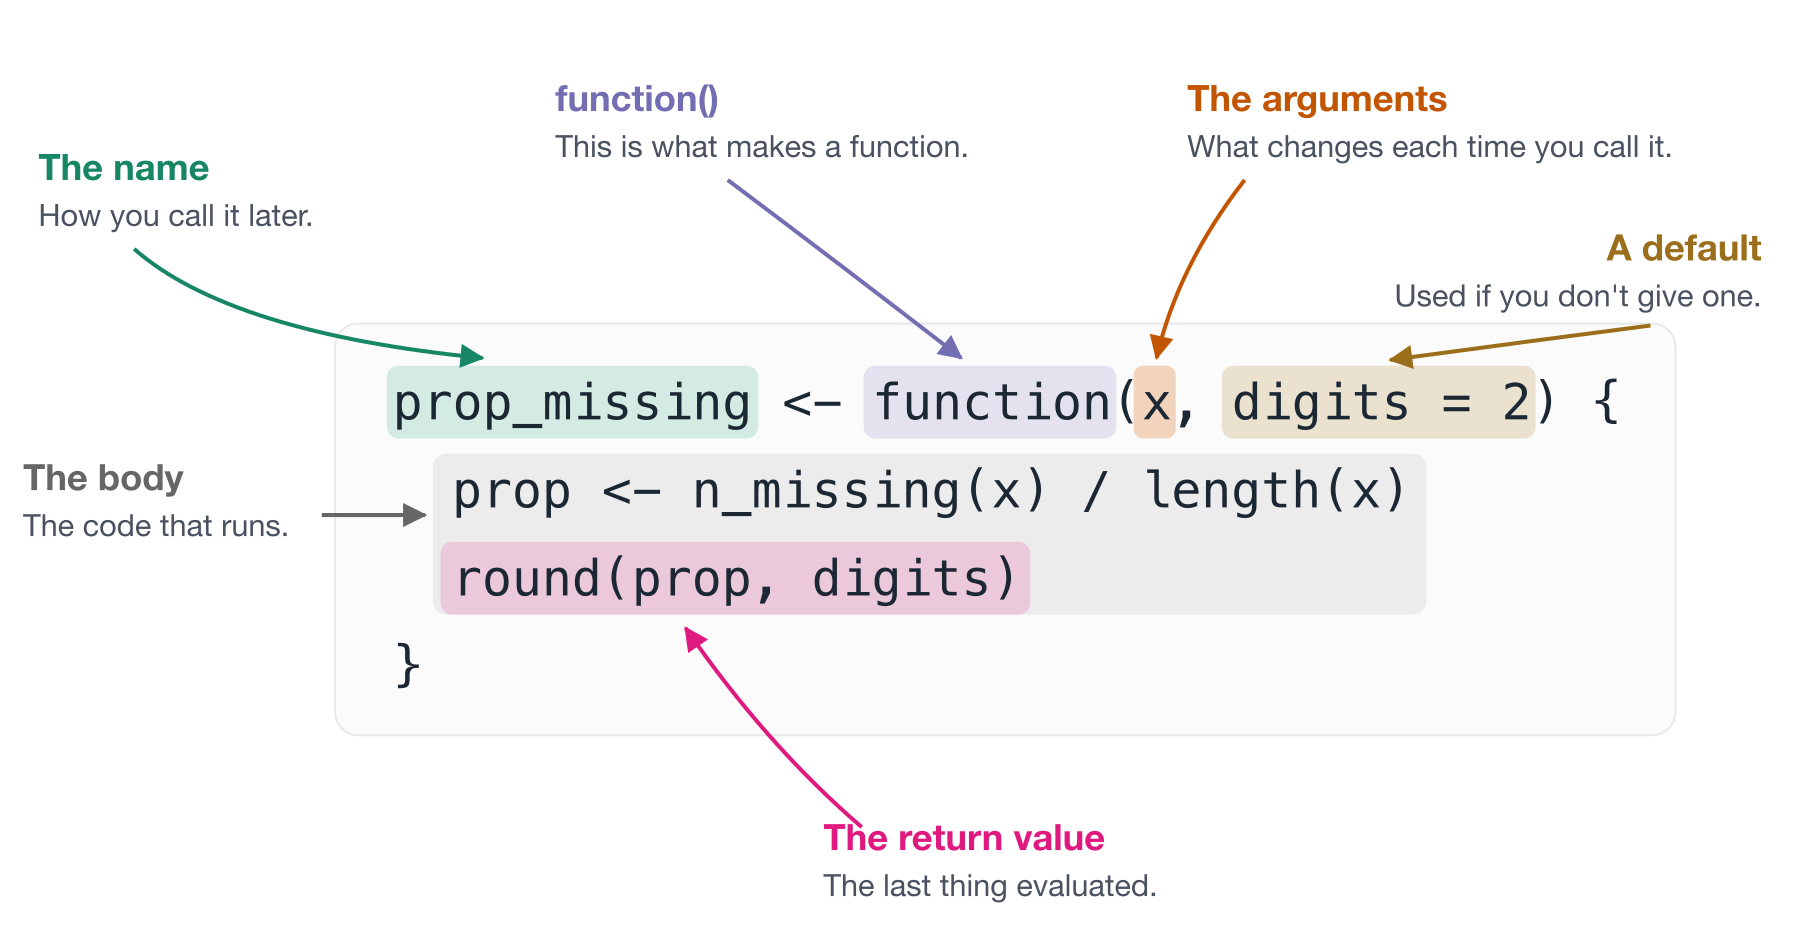
\includegraphics[width=1\linewidth,height=\textheight,keepaspectratio,alt={The function prop\_missing defined with function(x, digits = 2), with six parts highlighted in colour: the name, the function keyword, the argument x, the default digits = 2, the body, and the return value.}]{figs/function-anatomy.png}

}

\caption{The parts of a function.}

\end{figure}%

Taking the parts one at a time:

\begin{itemize}
\tightlist
\item
  \textbf{The name.} \texttt{prop\_missing}. This is how you call it
  later, so it is worth the two minutes it takes to pick a good one.
\item
  \textbf{\texttt{function()}.} This is the bit that actually creates a
  function. \texttt{prop\_missing\ \textless{}-} just binds it to a
  name, the same way you would bind any other value.
\item
  \textbf{The arguments.} \texttt{x} and \texttt{digits}. These are the
  things that change each time you call it. They are the answer to
  ``what did I keep editing at the top of my script?''
\item
  \textbf{A default.} \texttt{digits\ =\ 2}. If the caller doesn't
  supply \texttt{digits}, it is 2. Defaults let you make a function easy
  to call in the common case, without giving up control in the uncommon
  one.
\item
  \textbf{The body.} Everything between the braces. This is the code
  that runs.
\item
  \textbf{The return value.} R returns the \textbf{last thing
  evaluated}, so here that's the rounded proportion. You can write
  \texttt{return()} explicitly, and sometimes should for an early exit,
  but you don't have to.
\end{itemize}

The arguments are the part that trips people up, because \texttt{x} and
\texttt{digits} do not have values when you write the definition. They
are names waiting for something. The values arrive when you call the
function, and where they arrive is decided by the order you write them
in:

\begin{figure}[ht]

{\centering 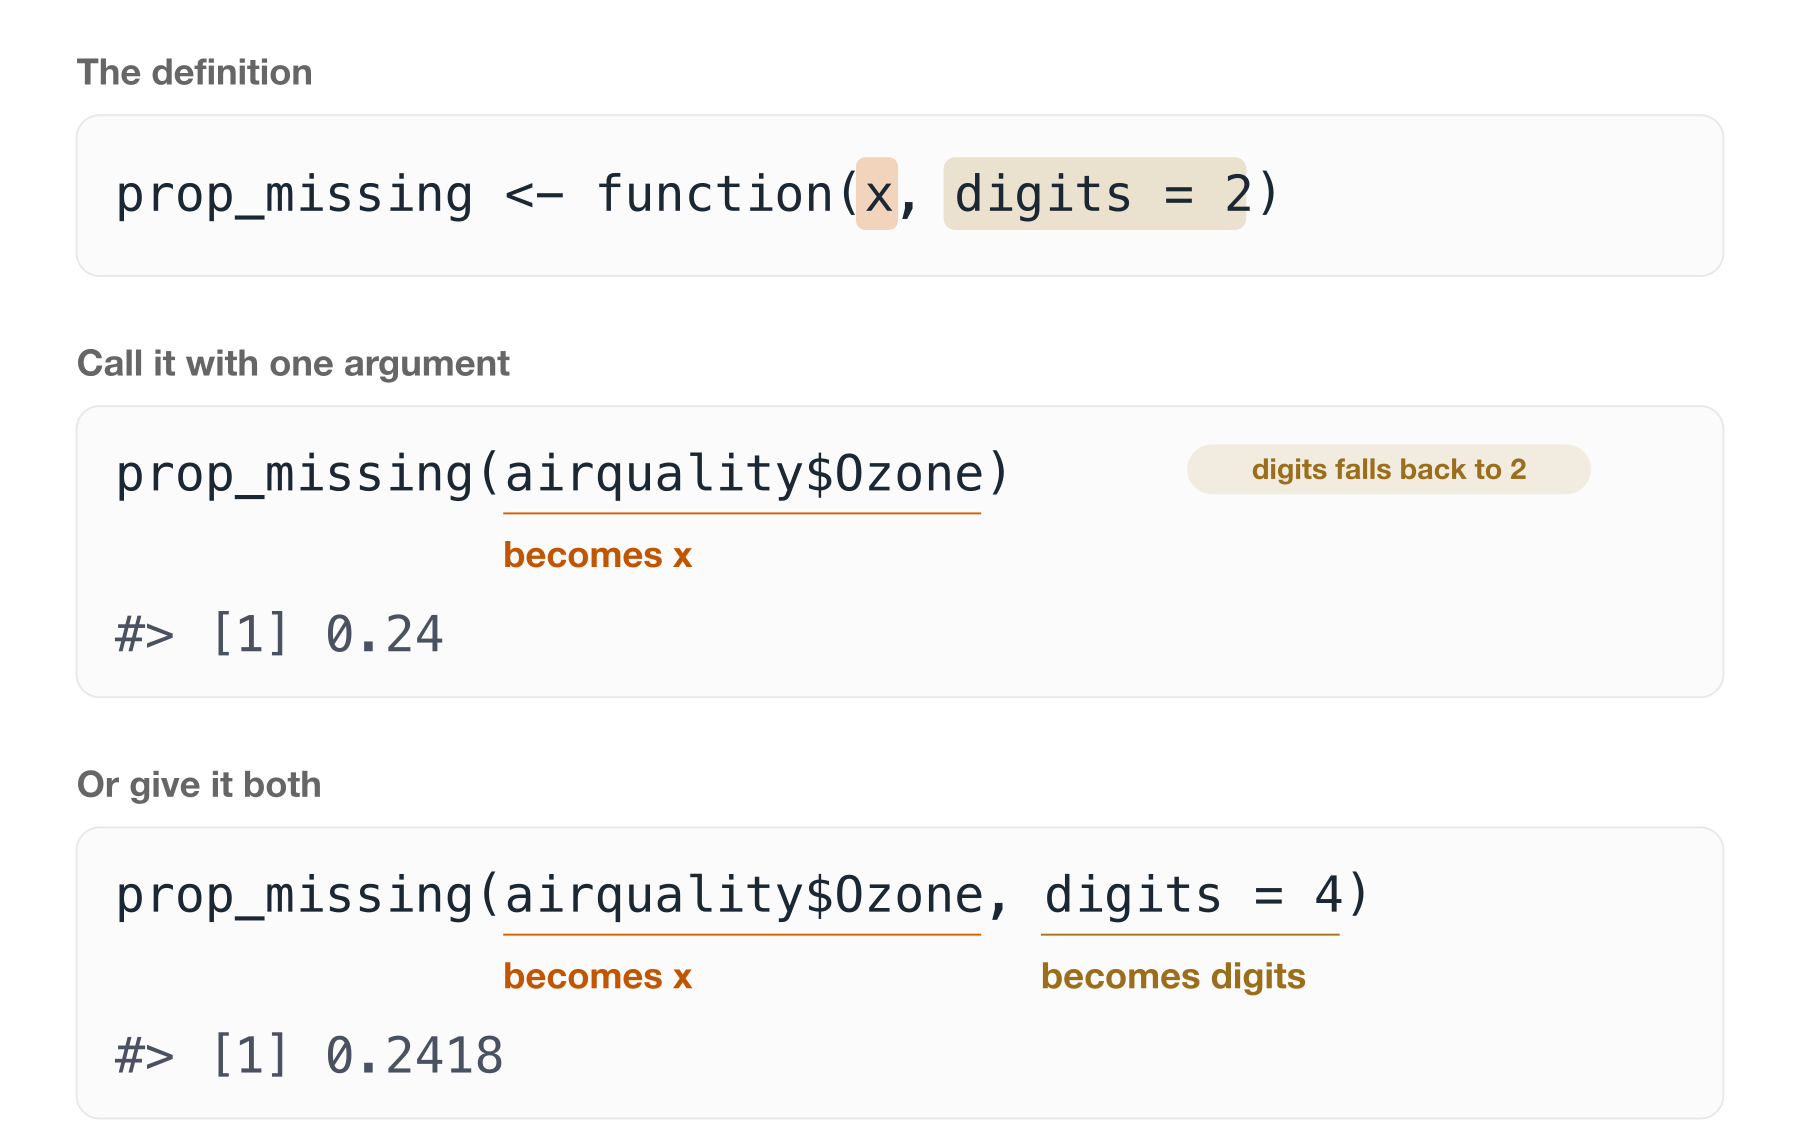
\includegraphics[width=1\linewidth,height=\textheight,keepaspectratio,alt={Three panels. The first shows the definition prop\_missing \textless- function(x, digits = 2), with x highlighted in orange and digits = 2 in brown. The second shows the call prop\_missing(airquality\$Ozone), with airquality\$Ozone underlined in orange and labelled \textquotesingle becomes x\textquotesingle, a badge noting that digits falls back to 2, and the result 0.24. The third shows prop\_missing(airquality\$Ozone, digits = 4), with airquality\$Ozone labelled \textquotesingle becomes x\textquotesingle{} and digits = 4 labelled \textquotesingle becomes digits\textquotesingle, returning 0.2418.}]{figs/function-in-use.png}

}

\caption{Argument values arrive at the call, not at the definition.}

\end{figure}%

The same function, two different answers, and nothing about the function
changed. That is the whole point of an argument.

\begin{tcolorbox}[enhanced jigsaw, arc=.35mm, bottomrule=.15mm, bottomtitle=1mm, breakable, colback=white, colbacktitle=quarto-callout-note-color!10!white, colframe=quarto-callout-note-color-frame, coltitle=black, left=2mm, leftrule=.75mm, opacityback=0, opacitybacktitle=0.6, rightrule=.15mm, title=\textcolor{quarto-callout-note-color}{\faInfo}\hspace{0.5em}{Your Turn}, titlerule=0mm, toprule=.15mm, toptitle=1mm]

Here is a function. Don't run it, and don't worry about what it
computes.

\begin{Shaded}
\begin{Highlighting}[]
\NormalTok{rate\_per\_1000 }\OtherTok{\textless{}{-}} \ControlFlowTok{function}\NormalTok{(count, population, }\AttributeTok{digits =} \DecValTok{1}\NormalTok{) \{}
\NormalTok{  rate }\OtherTok{\textless{}{-}}\NormalTok{ (count }\SpecialCharTok{/}\NormalTok{ population) }\SpecialCharTok{*} \DecValTok{1000}
  \FunctionTok{round}\NormalTok{(rate, digits)}
\NormalTok{\}}
\end{Highlighting}
\end{Shaded}

Name the parts:

\begin{enumerate}
\def\labelenumi{\arabic{enumi}.}
\tightlist
\item
  What is the \textbf{name} of this function?
\item
  What are its \textbf{arguments}?
\item
  Which argument has a \textbf{default}, and what is it?
\item
  What is the \textbf{body}?
\item
  What does it \textbf{return}?
\item
  Now call it two ways: once letting \texttt{digits} take its default,
  and once setting it yourself.
\end{enumerate}

The point of this one is the vocabulary. Once you can say ``the third
argument has a default'', you can look it up and you can ask about it.

\end{tcolorbox}

\begin{tcolorbox}[enhanced jigsaw, arc=.35mm, bottomrule=.15mm, bottomtitle=1mm, breakable, colback=white, colbacktitle=quarto-callout-tip-color!10!white, colframe=quarto-callout-tip-color-frame, coltitle=black, left=2mm, leftrule=.75mm, opacityback=0, opacitybacktitle=0.6, rightrule=.15mm, title=\textcolor{quarto-callout-tip-color}{\faLightbulb}\hspace{0.5em}{Two more parts, once the above is comfortable}, titlerule=0mm, toprule=.15mm, toptitle=1mm]

These are worth knowing about eventually. Skip them for now if you are
still getting the hang of the parts above.

\textbf{Side effects.} Anything a function does \emph{other} than return
a value. Printing to the console, writing a file, drawing a plot,
setting an option. Side effects are not bad, and plenty of useful
functions have them. But a function that both returns something useful
\emph{and} quietly writes a file is harder to reason about than one that
does a single one of those things.

\textbf{Functions are values.} An argument can be a function. Here is
the situation where you would want that.

Say you want to know how many values are missing in each column of your
data. With the function we already have, you could write:

\begin{Shaded}
\begin{Highlighting}[]
\FunctionTok{n\_missing}\NormalTok{(airquality}\SpecialCharTok{$}\NormalTok{Ozone)}
\FunctionTok{n\_missing}\NormalTok{(airquality}\SpecialCharTok{$}\NormalTok{Solar.R)}
\FunctionTok{n\_missing}\NormalTok{(airquality}\SpecialCharTok{$}\NormalTok{Wind)}
\FunctionTok{n\_missing}\NormalTok{(airquality}\SpecialCharTok{$}\NormalTok{Temp)}
\FunctionTok{n\_missing}\NormalTok{(airquality}\SpecialCharTok{$}\NormalTok{Month)}
\FunctionTok{n\_missing}\NormalTok{(airquality}\SpecialCharTok{$}\NormalTok{Day)}
\end{Highlighting}
\end{Shaded}

That is six lines to say one thing. You have to know every column name,
you have to type each one correctly, and when the data gains a column
next month you have to remember to come back and add a line.

It is the copy-paste problem from the start of this chapter, wearing a
different hat.

What you want to say is ``do this to every column''. To say that, you
need to hand one function to another function:

\begin{Shaded}
\begin{Highlighting}[]
\FunctionTok{library}\NormalTok{(purrr)}

\FunctionTok{map\_int}\NormalTok{(airquality, n\_missing)}
\end{Highlighting}
\end{Shaded}

\begin{verbatim}
  Ozone Solar.R    Wind    Temp   Month     Day 
     37       7       0       0       0       0 
\end{verbatim}

One line, and it does not care how many columns there are or what they
are called.

Look closely at how \texttt{n\_missing} is written there. \textbf{No
brackets.} We are not calling it, we are handing it over, the same way
we would hand over a number or a data frame. That is what ``functions
are values'' means.

And you can accept a function in your own functions too:

\begin{Shaded}
\begin{Highlighting}[]
\NormalTok{n\_complete }\OtherTok{\textless{}{-}} \ControlFlowTok{function}\NormalTok{(x) \{}
  \FunctionTok{sum}\NormalTok{(}\SpecialCharTok{!}\FunctionTok{is.na}\NormalTok{(x))}
\NormalTok{\}}

\NormalTok{summarise\_columns }\OtherTok{\textless{}{-}} \ControlFlowTok{function}\NormalTok{(data, f) \{}
  \FunctionTok{map\_dbl}\NormalTok{(data, f)}
\NormalTok{\}}

\FunctionTok{summarise\_columns}\NormalTok{(airquality, n\_complete)}
\end{Highlighting}
\end{Shaded}

\begin{verbatim}
  Ozone Solar.R    Wind    Temp   Month     Day 
    116     146     153     153     153     153 
\end{verbatim}

\begin{quote}
\textbf{A quick word on \texttt{map()}}

\href{https://purrr.tidyverse.org/}{\texttt{purrr}} is the tidyverse
package for applying a function to each element of something. The whole
family works the same way, and the suffix tells you what comes back:

\begin{itemize}
\tightlist
\item
  \texttt{map()} gives you a \textbf{list}, always.
\item
  \texttt{map\_int()} gives you an \textbf{integer vector}, or an error.
\item
  \texttt{map\_dbl()}, \texttt{map\_chr()}, \texttt{map\_lgl()} do the
  same for numbers, text and \texttt{TRUE}/\texttt{FALSE}.
\end{itemize}

That ``or an error'' is the point. You say what shape you are expecting,
and if the function cannot deliver it you find out straight away, rather
than three lines later when something else breaks.

\begin{Shaded}
\begin{Highlighting}[]
\FunctionTok{map\_dbl}\NormalTok{(airquality, as.character)}
\CommentTok{\#\textgreater{} Error in \textasciigrave{}map\_dbl()\textasciigrave{}:}
\CommentTok{\#\textgreater{} i In index: 1.}
\CommentTok{\#\textgreater{} i With name: Ozone.}
\CommentTok{\#\textgreater{} Caused by error:}
\CommentTok{\#\textgreater{} ! Result must be length 1, not 153.}
\end{Highlighting}
\end{Shaded}

Base R has its own versions of these, called \texttt{lapply()},
\texttt{vapply()} and \texttt{sapply()}. You will meet them in other
people's code, they do the same job with different names, and we will
come to the differences later.
\end{quote}

\begin{quote}
\textbf{Anonymous functions, and that \texttt{\textbackslash{}(x)}
thing}

Everything so far has handed over a function that already had a name.
Sometimes you want to hand over a function you will never need again,
where naming it would just add clutter to the top of your script.

You can write the function right there, in the argument:

\begin{Shaded}
\begin{Highlighting}[]
\FunctionTok{map\_dbl}\NormalTok{(airquality, }\ControlFlowTok{function}\NormalTok{(x) }\FunctionTok{round}\NormalTok{(}\FunctionTok{mean}\NormalTok{(x, }\AttributeTok{na.rm =} \ConstantTok{TRUE}\NormalTok{), }\DecValTok{1}\NormalTok{))}
\end{Highlighting}
\end{Shaded}

\begin{verbatim}
  Ozone Solar.R    Wind    Temp   Month     Day 
   42.1   185.9    10.0    77.9     7.0    15.8 
\end{verbatim}

That \texttt{function(x)\ round(mean(x,\ na.rm\ =\ TRUE),\ 1)} is an
ordinary function. It simply never got a name, which is why it is called
an \textbf{anonymous function}.

It does the same job as this:

\begin{Shaded}
\begin{Highlighting}[]
\NormalTok{mean\_rounded }\OtherTok{\textless{}{-}} \ControlFlowTok{function}\NormalTok{(x) \{}
  \FunctionTok{round}\NormalTok{(}\FunctionTok{mean}\NormalTok{(x, }\AttributeTok{na.rm =} \ConstantTok{TRUE}\NormalTok{), }\DecValTok{1}\NormalTok{)}
\NormalTok{\}}

\FunctionTok{map\_dbl}\NormalTok{(airquality, mean\_rounded)}
\end{Highlighting}
\end{Shaded}

\begin{verbatim}
  Ozone Solar.R    Wind    Temp   Month     Day 
   42.1   185.9    10.0    77.9     7.0    15.8 
\end{verbatim}

So which should you write? My rule is straightforward. If you would use
it twice, or if a name would explain something, give it a name.
Otherwise, leave it anonymous.

While you are learning, name them. A named function is something you can
call on its own and poke at, which makes it far easier to debug.

\textbf{The shorthand: \texttt{\textbackslash{}(x)}}

Since R 4.1 you can write \texttt{\textbackslash{}(x)} instead of
\texttt{function(x)}:

\begin{Shaded}
\begin{Highlighting}[]
\FunctionTok{map\_dbl}\NormalTok{(airquality, \textbackslash{}(x) }\FunctionTok{round}\NormalTok{(}\FunctionTok{mean}\NormalTok{(x, }\AttributeTok{na.rm =} \ConstantTok{TRUE}\NormalTok{), }\DecValTok{1}\NormalTok{))}
\end{Highlighting}
\end{Shaded}

\begin{verbatim}
  Ozone Solar.R    Wind    Temp   Month     Day 
   42.1   185.9    10.0    77.9     7.0    15.8 
\end{verbatim}

Identical to the version above, just shorter.
\texttt{\textbackslash{}(x)\ x\ +\ 1} and \texttt{function(x)\ x\ +\ 1}
are the same thing.

You will see \texttt{\textbackslash{}(x)} constantly in modern R code,
so it is worth being able to read. When you are writing your own, use
whichever you find clearer.
\end{quote}

\begin{quote}
\textbf{Some history: where the backslash comes from}

\texttt{\textbackslash{}(x)} is written with a backslash because it
looks a little like \textbf{λ}, the Greek letter lambda.

That comes from
\href{https://en.wikipedia.org/wiki/Lambda_calculus}{lambda calculus}, a
way of describing computation worked out by
\href{https://en.wikipedia.org/wiki/Alonzo_Church}{Alonzo Church} in the
1930s, where \texttt{λx.} means ``a function of x''.

Plenty of programming languages borrowed the idea and the word, which is
why you will hear anonymous functions called ``lambdas'' in Python,
JavaScript and elsewhere.
\end{quote}

\begin{quote}
\textbf{Some history: older purrr code and the
\texttt{\textasciitilde{}\ .x} shorthand}

In older code, and in plenty of code still being written today, you will
see this instead:

\begin{Shaded}
\begin{Highlighting}[]
\FunctionTok{map\_dbl}\NormalTok{(airquality, }\SpecialCharTok{\textasciitilde{}} \FunctionTok{round}\NormalTok{(}\FunctionTok{mean}\NormalTok{(.x, }\AttributeTok{na.rm =} \ConstantTok{TRUE}\NormalTok{), }\DecValTok{1}\NormalTok{))}
\end{Highlighting}
\end{Shaded}

\begin{verbatim}
  Ozone Solar.R    Wind    Temp   Month     Day 
   42.1   185.9    10.0    77.9     7.0    15.8 
\end{verbatim}

That \texttt{\textasciitilde{}} is a \textbf{formula}, and purrr treats
it as a shorthand for a function. Inside it, \texttt{.x} stands for
whatever is being passed in.

So all three of these do the same thing:

\begin{Shaded}
\begin{Highlighting}[]
\FunctionTok{map\_dbl}\NormalTok{(airquality, }\SpecialCharTok{\textasciitilde{}} \FunctionTok{round}\NormalTok{(}\FunctionTok{mean}\NormalTok{(.x, }\AttributeTok{na.rm =} \ConstantTok{TRUE}\NormalTok{), }\DecValTok{1}\NormalTok{))}
\FunctionTok{map\_dbl}\NormalTok{(airquality, \textbackslash{}(x) }\FunctionTok{round}\NormalTok{(}\FunctionTok{mean}\NormalTok{(x, }\AttributeTok{na.rm =} \ConstantTok{TRUE}\NormalTok{), }\DecValTok{1}\NormalTok{))}
\FunctionTok{map\_dbl}\NormalTok{(airquality, }\ControlFlowTok{function}\NormalTok{(x) }\FunctionTok{round}\NormalTok{(}\FunctionTok{mean}\NormalTok{(x, }\AttributeTok{na.rm =} \ConstantTok{TRUE}\NormalTok{), }\DecValTok{1}\NormalTok{))}
\end{Highlighting}
\end{Shaded}

The formula version came first, because until R 4.1 there was no short
way to write a function, and \texttt{function(x)} every time got tiring.
Now that \texttt{\textbackslash{}(x)} exists, purrr's own documentation
recommends it, and it is what I would write in new code.

You still need to be able to \emph{read} \texttt{\textasciitilde{}\ .x},
because it is everywhere.

Two more things you will meet alongside it. A bare \texttt{.} works in
place of \texttt{.x}, and in two-argument functions like \texttt{map2()}
the arguments are \texttt{.x} and \texttt{.y}:

\begin{Shaded}
\begin{Highlighting}[]
\FunctionTok{map2\_dbl}\NormalTok{(}\DecValTok{1}\SpecialCharTok{:}\DecValTok{3}\NormalTok{, }\DecValTok{4}\SpecialCharTok{:}\DecValTok{6}\NormalTok{, }\SpecialCharTok{\textasciitilde{}}\NormalTok{ .x }\SpecialCharTok{*}\NormalTok{ .y)}
\end{Highlighting}
\end{Shaded}

\begin{verbatim}
[1]  4 10 18
\end{verbatim}
\end{quote}

\end{tcolorbox}

\section{Good (simple) function
design}\label{good-simple-function-design}

Functions are \textbf{tools for managing complexity}. That is also
called \emph{abstraction}, or \emph{abstracting away}.

So the question when writing one is always: \textbf{what complexity am I
managing? What am I abstracting away?}

Here is a real piece of analysis code. It asks whether temperature
differs on days when ozone is missing, compared with days when it is
not:

\begin{Shaded}
\begin{Highlighting}[]
\NormalTok{is\_different }\OtherTok{\textless{}{-}}\NormalTok{ airquality}\SpecialCharTok{$}\NormalTok{Temp}
\NormalTok{when\_missing\_index }\OtherTok{\textless{}{-}} \FunctionTok{which}\NormalTok{(}\FunctionTok{is.na}\NormalTok{(airquality}\SpecialCharTok{$}\NormalTok{Ozone))}
\NormalTok{when\_complete\_index }\OtherTok{\textless{}{-}} \FunctionTok{which}\NormalTok{(}\SpecialCharTok{!}\FunctionTok{is.na}\NormalTok{(airquality}\SpecialCharTok{$}\NormalTok{Ozone))}
\NormalTok{is\_different\_miss }\OtherTok{\textless{}{-}}\NormalTok{ is\_different[when\_missing\_index]}
\NormalTok{is\_different\_complete }\OtherTok{\textless{}{-}}\NormalTok{ is\_different[when\_complete\_index]}
\NormalTok{result\_ozone\_temp }\OtherTok{\textless{}{-}} \FunctionTok{t.test}\NormalTok{(is\_different\_miss, is\_different\_complete)}
\end{Highlighting}
\end{Shaded}

That works. But you can't use it on another pair of variables without
editing it, and you can't tell at a glance what it's \emph{for}.

\textbf{Writing a function is writing.} You don't get it right on the
first pass, and you're not supposed to.

Here's the actual process.

\textbf{Start with the bones.} Make an empty function and paste the code
into the body.

\begin{Shaded}
\begin{Highlighting}[]
\NormalTok{misstest }\OtherTok{\textless{}{-}} \ControlFlowTok{function}\NormalTok{(Temp, Ozone) \{}
  \CommentTok{\# paste the text into the body}
\NormalTok{\}}
\end{Highlighting}
\end{Shaded}

\textbf{Ask what you are interested in.} Which parts change? Here it is
the variable we are testing, and the variable whose missingness we are
splitting on.

\textbf{Work out what to name things.} Replace the hard-coded
\texttt{airquality\$Temp} with an argument. Comment out the old line
rather than deleting it, so you can see what you are replacing:

\begin{Shaded}
\begin{Highlighting}[]
\NormalTok{misstest }\OtherTok{\textless{}{-}} \ControlFlowTok{function}\NormalTok{(is\_different, when\_missing) \{}
  \CommentTok{\# is\_different \textless{}{-} airquality$Temp}
\NormalTok{  when\_missing\_index }\OtherTok{\textless{}{-}} \FunctionTok{which}\NormalTok{(}\FunctionTok{is.na}\NormalTok{(when\_missing))}
\NormalTok{  when\_complete\_index }\OtherTok{\textless{}{-}} \FunctionTok{which}\NormalTok{(}\SpecialCharTok{!}\FunctionTok{is.na}\NormalTok{(when\_missing))}
\NormalTok{  is\_different\_miss }\OtherTok{\textless{}{-}}\NormalTok{ is\_different[when\_missing\_index]}
\NormalTok{  is\_different\_complete }\OtherTok{\textless{}{-}}\NormalTok{ is\_different[when\_complete\_index]}
\NormalTok{  result\_ozone\_temp }\OtherTok{\textless{}{-}} \FunctionTok{t.test}\NormalTok{(is\_different\_miss, is\_different\_complete)}
\NormalTok{\}}
\end{Highlighting}
\end{Shaded}

Naming is tricky, and it's fine for it to take a few goes.

\textbf{Return the last thing.} The function currently assigns to
\texttt{result\_ozone\_temp} and returns it invisibly. Put it on its own
line at the end so the return is explicit to a reader:

\begin{Shaded}
\begin{Highlighting}[]
\NormalTok{  result\_ozone\_temp }\OtherTok{\textless{}{-}} \FunctionTok{t.test}\NormalTok{(is\_different\_miss, is\_different\_complete)}
\NormalTok{  result\_ozone\_temp}
\ErrorTok{\}}
\end{Highlighting}
\end{Shaded}

\textbf{Clean up the old lettuce.} Remove the commented-out lines now
that you no longer need them.

\textbf{Name the function so it evokes the action.} \texttt{misstest}
was a placeholder. What does this actually do?

\begin{Shaded}
\begin{Highlighting}[]
\NormalTok{missingness\_impact }\OtherTok{\textless{}{-}} \ControlFlowTok{function}\NormalTok{(is\_different, when\_missing) \{}
\NormalTok{  when\_missing\_index }\OtherTok{\textless{}{-}} \FunctionTok{which}\NormalTok{(}\FunctionTok{is.na}\NormalTok{(when\_missing))}
\NormalTok{  when\_complete\_index }\OtherTok{\textless{}{-}} \FunctionTok{which}\NormalTok{(}\SpecialCharTok{!}\FunctionTok{is.na}\NormalTok{(when\_missing))}
\NormalTok{  is\_different\_miss }\OtherTok{\textless{}{-}}\NormalTok{ is\_different[when\_missing\_index]}
\NormalTok{  is\_different\_complete }\OtherTok{\textless{}{-}}\NormalTok{ is\_different[when\_complete\_index]}
  \FunctionTok{t.test}\NormalTok{(is\_different\_miss, is\_different\_complete)}
\NormalTok{\}}
\end{Highlighting}
\end{Shaded}

\textbf{Then use it}, and write the output to a variable:

\begin{Shaded}
\begin{Highlighting}[]
\NormalTok{temp\_difference\_ozone\_missing }\OtherTok{\textless{}{-}} \FunctionTok{missingness\_impact}\NormalTok{(}
  \AttributeTok{when\_missing =}\NormalTok{ airquality}\SpecialCharTok{$}\NormalTok{Ozone,}
  \AttributeTok{is\_different =}\NormalTok{ airquality}\SpecialCharTok{$}\NormalTok{Temp}
\NormalTok{)}
\end{Highlighting}
\end{Shaded}

The process, in short:

\begin{enumerate}
\def\labelenumi{\arabic{enumi}.}
\tightlist
\item
  \textbf{Copy} the text into the body.
\item
  \textbf{Identify} the complexity to manage.
\item
  \textbf{Abstract} that complexity.
\item
  \textbf{Iterate} --- writing functions is iterative, just like regular
  writing.
\end{enumerate}

\begin{tcolorbox}[enhanced jigsaw, arc=.35mm, bottomrule=.15mm, bottomtitle=1mm, breakable, colback=white, colbacktitle=quarto-callout-tip-color!10!white, colframe=quarto-callout-tip-color-frame, coltitle=black, left=2mm, leftrule=.75mm, opacityback=0, opacitybacktitle=0.6, rightrule=.15mm, title=\textcolor{quarto-callout-tip-color}{\faLightbulb}\hspace{0.5em}{Circling back to DRY}, titlerule=0mm, toprule=.15mm, toptitle=1mm]

You will often be told: ``if you copy and paste the same code three
times, write a function.''

That's true, but it treats the symptom. The real problem is
\textbf{complex code}.

You only end up repeating yourself because you couldn't \emph{express}
the idea. So the cause is expression and reasoning, not repetition.

A function isn't only needed when you repeat code. It's needed when you
have an idea worth naming.

\end{tcolorbox}

\begin{tcolorbox}[enhanced jigsaw, arc=.35mm, bottomrule=.15mm, bottomtitle=1mm, breakable, colback=white, colbacktitle=quarto-callout-note-color!10!white, colframe=quarto-callout-note-color-frame, coltitle=black, left=2mm, leftrule=.75mm, opacityback=0, opacitybacktitle=0.6, rightrule=.15mm, title=\textcolor{quarto-callout-note-color}{\faInfo}\hspace{0.5em}{Your Turn}, titlerule=0mm, toprule=.15mm, toptitle=1mm]

Earlier you wrote down a sentence describing a chunk of your own code.
Now build the function around it, using the process above.

\begin{enumerate}
\def\labelenumi{\arabic{enumi}.}
\tightlist
\item
  \textbf{Copy.} Make an empty function, and paste the chunk into the
  body. Don't change anything yet.
\item
  \textbf{Identify.} Which parts of it change between uses? Those are
  your arguments.
\item
  \textbf{Abstract.} Replace the hard-coded parts with argument names.
  Comment the old lines out rather than deleting them, so you can see
  what you are replacing.
\item
  \textbf{Iterate.} Get it working first, then go back and improve the
  names. The first name you pick is rarely the one you keep.
\end{enumerate}

Then call your function, and check you get the same answer you got
before you started. That check matters. It is very easy to tidy
something into a different result.

If you don't have a chunk of your own to hand, use
\texttt{06-bad-style/messy-analysis.R} from the course repository. The
loop at the bottom is doing the same thing to each species, one at a
time.

\end{tcolorbox}

\section{Using \{fnmate\} to speed up creating
functions}\label{using-fnmate-to-speed-up-creating-functions}

The process above has one annoying step. You write the call you
\emph{wish} existed, then go and create the function somewhere else,
with the right arguments, and switch back.

\href{https://github.com/milesmcbain/fnmate}{\texttt{\{fnmate\}}} by
Miles McBain removes that step. Write the call you want:

\begin{Shaded}
\begin{Highlighting}[]
\NormalTok{temp\_difference }\OtherTok{\textless{}{-}} \FunctionTok{missingness\_impact}\NormalTok{(}
  \AttributeTok{when\_missing =}\NormalTok{ airquality}\SpecialCharTok{$}\NormalTok{Ozone,}
  \AttributeTok{is\_different =}\NormalTok{ airquality}\SpecialCharTok{$}\NormalTok{Temp}
\NormalTok{)}
\end{Highlighting}
\end{Shaded}

Put your cursor on it, trigger \texttt{\{fnmate\}}, and it generates the
function definition --- correctly named, with the right argument names
--- in your \texttt{R/} directory, ready for you to fill in the body.

This matters more than a keystroke saving. It makes the
\textbf{outside-in} approach cheap. You imagine the interface you want
first, then write the thing that satisfies it.

Without tooling, outside-in is enough extra effort that most people
default to inside-out.

\begin{tcolorbox}[enhanced jigsaw, arc=.35mm, bottomrule=.15mm, bottomtitle=1mm, breakable, colback=white, colbacktitle=quarto-callout-note-color!10!white, colframe=quarto-callout-note-color-frame, coltitle=black, left=2mm, leftrule=.75mm, opacityback=0, opacitybacktitle=0.6, rightrule=.15mm, title=\textcolor{quarto-callout-note-color}{\faInfo}\hspace{0.5em}{Your Turn}, titlerule=0mm, toprule=.15mm, toptitle=1mm]

\begin{enumerate}
\def\labelenumi{\arabic{enumi}.}
\tightlist
\item
  Install it with
  \texttt{remotes::install\_github("milesmcbain/fnmate")}. If the
  install gives you trouble, skip it and do the rest by hand. The habit
  is the point, not the package.
\item
  Think of something you want to do but haven't written yet. Write
  \textbf{only the call}, with the argument names you wish existed.
\item
  Read what you wrote back. Could someone else tell what it does from
  the call alone? If not, rename things now, while it costs you nothing.
\item
  Now generate the function, with \texttt{\{fnmate\}} or by hand, and
  fill in the body.
\end{enumerate}

Notice the order you just worked in. You designed the interface first
and the implementation second, which is the opposite of how most of us
write code.

\end{tcolorbox}

\section{How to use a debugger}\label{how-to-use-a-debugger}

R is interactive. You run some code, you see the output immediately, and
when something goes wrong you can poke around and look at it. It is a
lovely way to do data analysis.

Functions break that. A function is a box, and by default you can't see
inside it while it runs.

To look inside, you need a debugger.

\begin{tcolorbox}[enhanced jigsaw, arc=.35mm, bottomrule=.15mm, bottomtitle=1mm, breakable, colback=white, colbacktitle=quarto-callout-caution-color!10!white, colframe=quarto-callout-caution-color-frame, coltitle=black, left=2mm, leftrule=.75mm, opacityback=0, opacitybacktitle=0.6, rightrule=.15mm, title=\textcolor{quarto-callout-caution-color}{\faFire}\hspace{0.5em}{A confession}, titlerule=0mm, toprule=.15mm, toptitle=1mm]

If you have ever copied the internals of a function into a new script,
hard-coded the arguments at the top, and run it line by line --- this
section is for you.

I say that as someone who did exactly that for years.

\end{tcolorbox}

Three tools to know:

\textbf{\texttt{browser()}} goes \emph{inside} a function. When you run
the function, you land at that point in the code:

\begin{Shaded}
\begin{Highlighting}[]
\NormalTok{mean\_center }\OtherTok{\textless{}{-}} \ControlFlowTok{function}\NormalTok{(variable) \{}
  \FunctionTok{browser}\NormalTok{()}
\NormalTok{  variable }\SpecialCharTok{{-}} \FunctionTok{mean}\NormalTok{(variable, }\AttributeTok{na.rm =} \ConstantTok{TRUE}\NormalTok{)}
\NormalTok{\}}
\end{Highlighting}
\end{Shaded}

Run that, then call \texttt{mean\_center(1:10)}, and you'll be dropped
in at the \texttt{browser()} line with \texttt{variable} available to
inspect.

The important thing to remember is that you have to \textbf{remove
\texttt{browser()} afterwards}.

\textbf{\texttt{debug()} and \texttt{undebug()}} do the same job without
editing the function. \texttt{debug()} turns on debugging mode for a
function --- as though \texttt{browser()} were on its first line:

\begin{Shaded}
\begin{Highlighting}[]
\FunctionTok{debug}\NormalTok{(mean\_center)}
\FunctionTok{mean\_center}\NormalTok{(}\DecValTok{1}\SpecialCharTok{:}\DecValTok{10}\NormalTok{)}
\CommentTok{\# poke around, inspect the values}
\FunctionTok{undebug}\NormalTok{(mean\_center)}
\end{Highlighting}
\end{Shaded}

\textbf{\texttt{debugonce()}} does the \texttt{debug()} step exactly
once, so you never need to call \texttt{undebug()}.

This matters more than it sounds. I've forgotten to call
\texttt{undebug()} and felt a genuine madness descend as every
subsequent call dropped me into the debugger.

So: if you want to see where a function is going wrong, reach for
\texttt{debugonce()}.

\begin{tcolorbox}[enhanced jigsaw, arc=.35mm, bottomrule=.15mm, bottomtitle=1mm, breakable, colback=white, colbacktitle=quarto-callout-note-color!10!white, colframe=quarto-callout-note-color-frame, coltitle=black, left=2mm, leftrule=.75mm, opacityback=0, opacitybacktitle=0.6, rightrule=.15mm, title=\textcolor{quarto-callout-note-color}{\faInfo}\hspace{0.5em}{Your Turn}, titlerule=0mm, toprule=.15mm, toptitle=1mm]

Here is \texttt{prop\_missing()} again, with one small change. It still
runs, and it still gives you a plausible looking number. It is wrong.

\begin{Shaded}
\begin{Highlighting}[]
\NormalTok{n\_missing }\OtherTok{\textless{}{-}} \ControlFlowTok{function}\NormalTok{(x) \{}
  \FunctionTok{sum}\NormalTok{(}\FunctionTok{is.na}\NormalTok{(x))}
\NormalTok{\}}

\NormalTok{prop\_missing }\OtherTok{\textless{}{-}} \ControlFlowTok{function}\NormalTok{(x, }\AttributeTok{digits =} \DecValTok{2}\NormalTok{) \{}
\NormalTok{  prop }\OtherTok{\textless{}{-}} \FunctionTok{n\_missing}\NormalTok{(x) }\SpecialCharTok{/} \FunctionTok{length}\NormalTok{(}\FunctionTok{na.omit}\NormalTok{(x))}
  \FunctionTok{round}\NormalTok{(prop, digits)}
\NormalTok{\}}

\FunctionTok{prop\_missing}\NormalTok{(airquality}\SpecialCharTok{$}\NormalTok{Ozone)}
\end{Highlighting}
\end{Shaded}

\begin{enumerate}
\def\labelenumi{\arabic{enumi}.}
\tightlist
\item
  Run it. You get \texttt{0.32}. Earlier in this chapter the answer was
  \texttt{0.24}. Which is right?
\item
  Run \texttt{debugonce(prop\_missing)}, then call it again. You will
  land inside the function.
\item
  Step forward one line at a time by typing \texttt{n} and pressing
  enter. At any point, type the name of a variable to see what it
  currently holds.
\item
  Type \texttt{length(x)} and then \texttt{length(na.omit(x))}. What is
  the difference between them, and which one belongs in a proportion?
\item
  Type \texttt{Q} to quit the debugger, fix the function, and run it
  again.
\end{enumerate}

This is the kind of bug worth practising on. Nothing errors, nothing
warns you, and \texttt{0.32} is every bit as believable as
\texttt{0.24}.

Then do the same on a function of your own that you don't entirely
trust.

The habit worth building: when a function surprises you, your first move
is \texttt{debugonce()}, not copying the body into a new script.

\end{tcolorbox}

\begin{tcolorbox}[enhanced jigsaw, arc=.35mm, bottomrule=.15mm, bottomtitle=1mm, breakable, colback=white, colbacktitle=quarto-callout-tip-color!10!white, colframe=quarto-callout-tip-color-frame, coltitle=black, left=2mm, leftrule=.75mm, opacityback=0, opacitybacktitle=0.6, rightrule=.15mm, title=\textcolor{quarto-callout-tip-color}{\faLightbulb}\hspace{0.5em}{Read more}, titlerule=0mm, toprule=.15mm, toptitle=1mm]

Parts of this chapter are adapted from my blog post,
\href{https://www.njtierney.com/posts/2023-10-30-how-to-get-good-with-r/}{How
to get good with R}.

The function design walkthrough, and the argument that DRY treats the
symptom rather than the cause, come from my talk \textbf{Practical
functions: practically magic} ---
\href{https://njtierney.github.io/funfun/\#/title-slide}{slides} and
\href{https://github.com/njtierney/funfun}{source}.

Its take-home messages are worth repeating here. Good functions:

\begin{enumerate}
\def\labelenumi{\arabic{enumi}.}
\tightlist
\item
  Manage \textbf{complexity}
\item
  Explain and express \textbf{ideas}
\item
  Can be \textbf{individually reasoned} with
\item
  Take \textbf{iteration}
\end{enumerate}

\end{tcolorbox}

\bookmarksetup{startatroot}

\chapter{Writing a reprex / getting
unstuck}\label{writing-a-reprex-getting-unstuck-1}

Everyone gets stuck. The skill is not avoiding it, it is getting unstuck
quickly, and being able to ask for help in a way that actually gets you
an answer.

This section is about the reproducible example, or reprex. We look at
how to build one, why building one so often solves the problem before
you ask anybody, and some practical habits for debugging.

\section{Overview}\label{overview-4}

\begin{itemize}
\tightlist
\item
  \textbf{Duration} 15 minutes
\end{itemize}

\section{Questions}\label{questions-4}

\section{How to share problems}\label{how-to-share-problems}

When you hit an error you cannot solve by tinkering, it is worth
spending some time building a small example of the code that breaks.

This takes practice. And here's the thing nobody tells you.

\textbf{In the process of reducing the problem to its core, you'll often
solve it yourself.}

It's the same experience as describing a problem out loud to a colleague
and arriving at the answer before they've said anything.

So a reprex isn't only a way to ask for help. It's a debugging technique
that happens to produce something shareable.

Let's tear one down. Say we are summarising the \texttt{diamonds} data:

\begin{Shaded}
\begin{Highlighting}[]
\FunctionTok{library}\NormalTok{(tidyverse)}

\NormalTok{diamonds }\SpecialCharTok{|\textgreater{}}
  \FunctionTok{mutate}\NormalTok{(}\AttributeTok{price\_per\_carat =}\NormalTok{ price }\SpecialCharTok{/}\NormalTok{ carat) }\SpecialCharTok{|\textgreater{}}
  \FunctionTok{group\_by}\NormalTok{(cut) }\SpecialCharTok{|\textgreater{}}
  \FunctionTok{summarise}\NormalTok{(}
    \AttributeTok{price\_mean =} \FunctionTok{mean}\NormalTok{(price\_per\_carat),}
    \AttributeTok{price\_sd =} \FunctionTok{sd}\NormalTok{(price\_per\_carat),}
    \AttributeTok{mean\_color =} \FunctionTok{mean}\NormalTok{(color)}
\NormalTok{  )}
\CommentTok{\#\textgreater{} Warning: There were 5 warnings in \textasciigrave{}summarise()\textasciigrave{}.}
\CommentTok{\#\textgreater{} The first warning was:}
\CommentTok{\#\textgreater{} ℹ In argument: \textasciigrave{}mean\_color = mean(color)\textasciigrave{}.}
\CommentTok{\#\textgreater{} ℹ In group 1: \textasciigrave{}cut = Fair\textasciigrave{}.}
\CommentTok{\#\textgreater{} Caused by warning in \textasciigrave{}mean.default()\textasciigrave{}:}
\CommentTok{\#\textgreater{} ! argument is not numeric or logical: returning NA}
\end{Highlighting}
\end{Shaded}

The warning gives us a clue: it is something about \texttt{mean\_color}.
So try just that:

\begin{Shaded}
\begin{Highlighting}[]
\NormalTok{diamonds }\SpecialCharTok{|\textgreater{}}
  \FunctionTok{mutate}\NormalTok{(}\AttributeTok{mean\_color =} \FunctionTok{mean}\NormalTok{(color))}
\CommentTok{\#\textgreater{} Warning: There was 1 warning in \textasciigrave{}mutate()\textasciigrave{}.}
\CommentTok{\#\textgreater{} ℹ In argument: \textasciigrave{}mean\_color = mean(color)\textasciigrave{}.}
\CommentTok{\#\textgreater{} Caused by warning in \textasciigrave{}mean.default()\textasciigrave{}:}
\CommentTok{\#\textgreater{} ! argument is not numeric or logical: returning NA}
\end{Highlighting}
\end{Shaded}

Same warning, and we've dropped \texttt{group\_by()} and
\texttt{summarise()} entirely. Strip it further:

\begin{Shaded}
\begin{Highlighting}[]
\FunctionTok{mean}\NormalTok{(diamonds}\SpecialCharTok{$}\NormalTok{color)}
\CommentTok{\#\textgreater{} Warning in mean.default(diamonds$color): argument is not numeric or}
\CommentTok{\#\textgreater{} logical: returning NA}
\CommentTok{\#\textgreater{} [1] NA}
\end{Highlighting}
\end{Shaded}

Still the same. We are now down to one line. So what is in
\texttt{color}?

\begin{Shaded}
\begin{Highlighting}[]
\FunctionTok{head}\NormalTok{(diamonds}\SpecialCharTok{$}\NormalTok{color)}
\CommentTok{\#\textgreater{} [1] E E E I J J}
\CommentTok{\#\textgreater{} Levels: D \textless{} E \textless{} F \textless{} G \textless{} H \textless{} I \textless{} J}
\end{Highlighting}
\end{Shaded}

Ah. Does it make sense to take the mean of some letters? Of course not.

Notice what happened. We never needed to ask anyone.

Each step made the example smaller, and the smaller it got, the more
obvious the problem became.

That's the technique.

\begin{figure}[ht]

{\centering 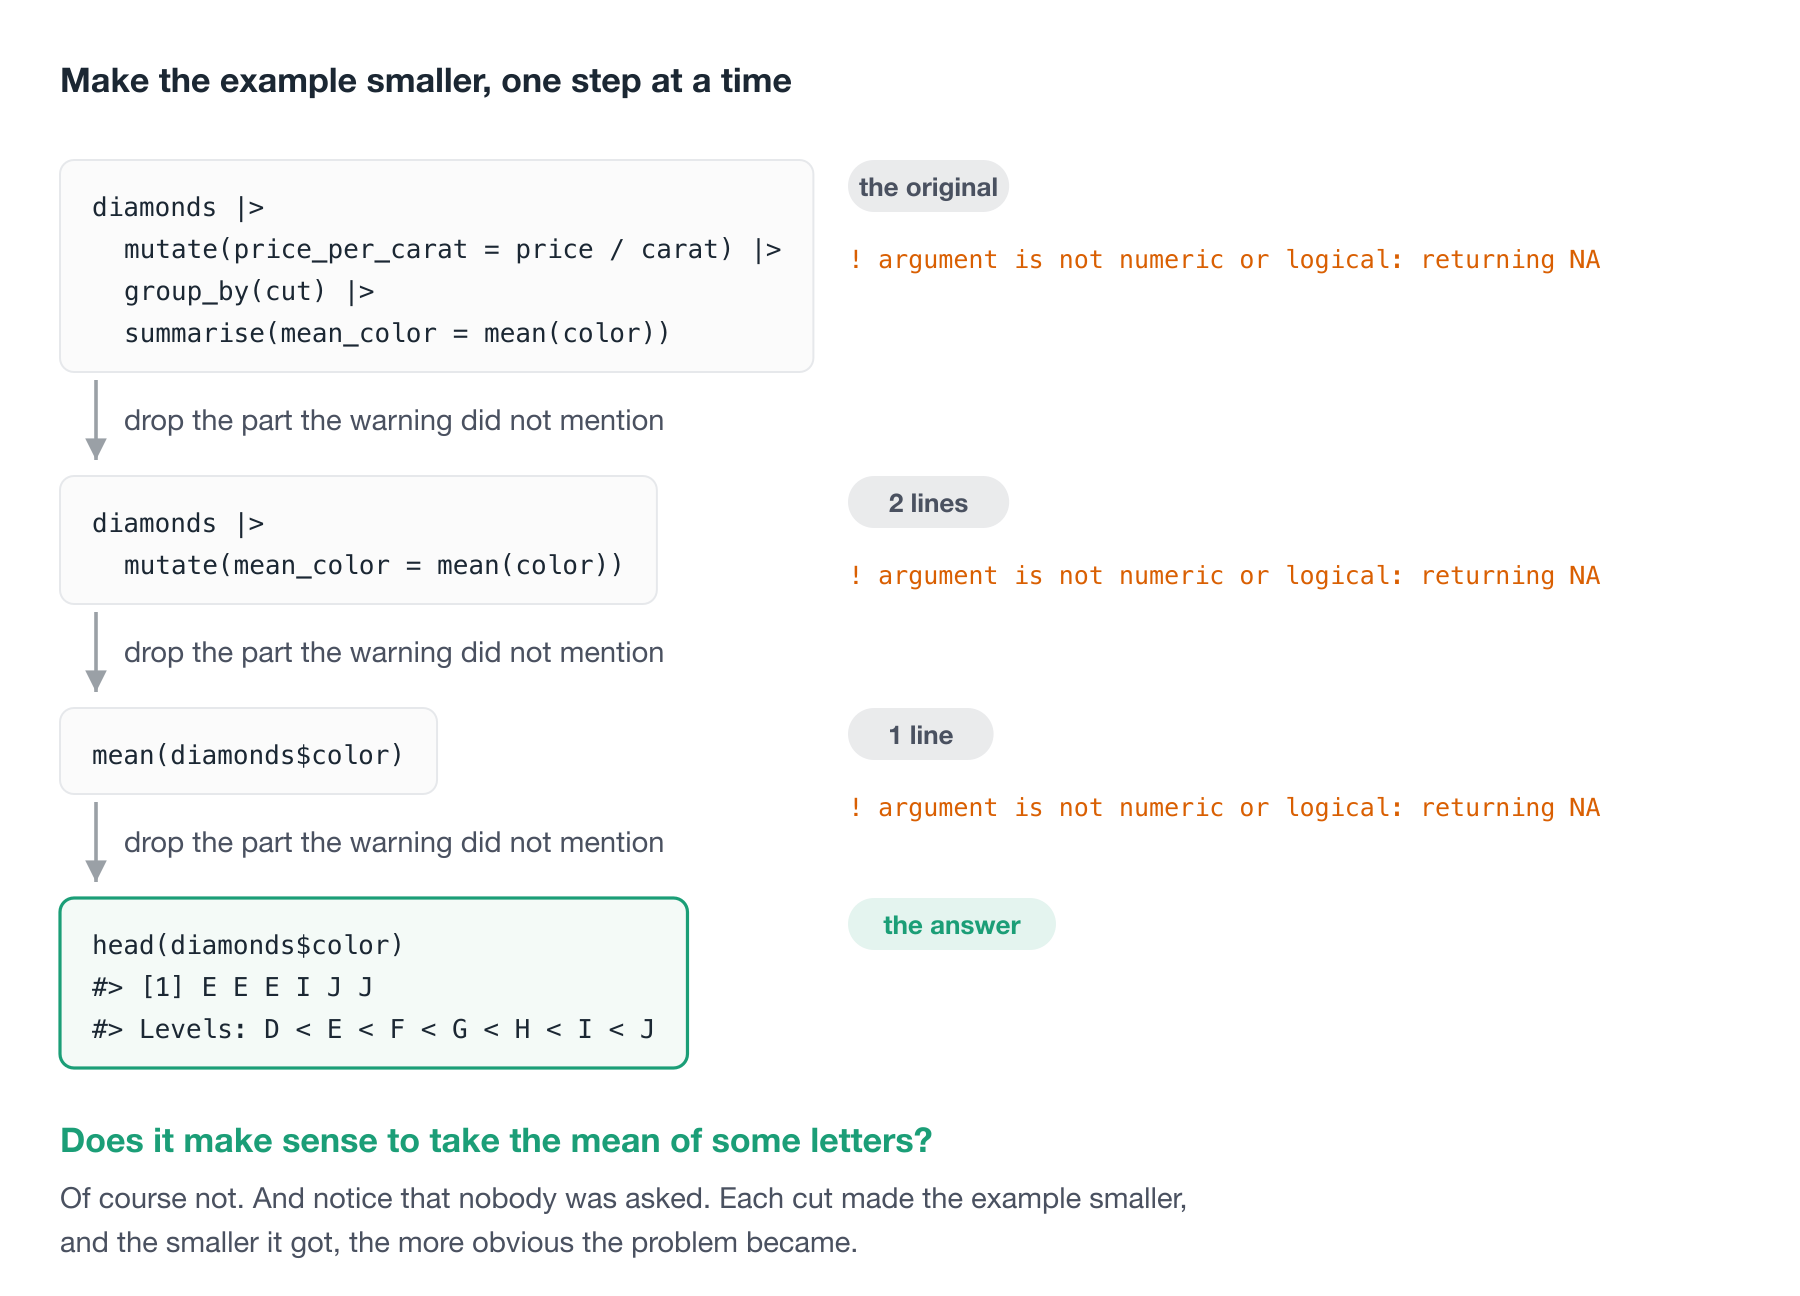
\includegraphics[width=1\linewidth,height=\textheight,keepaspectratio,alt={Four steps. An eight line pipeline warns that an argument is not numeric or logical. Dropping group\_by and summarise gives the same warning from two lines. Dropping mutate gives the same warning from one line. Finally, looking at the column shows it is a factor, so taking its mean was never going to work. The answer arrived without anyone being asked.}]{figs/reprex-reduction.png}

}

\caption{Cutting the example down until the problem is obvious.}

\end{figure}%

\begin{tcolorbox}[enhanced jigsaw, arc=.35mm, bottomrule=.15mm, bottomtitle=1mm, breakable, colback=white, colbacktitle=quarto-callout-note-color!10!white, colframe=quarto-callout-note-color-frame, coltitle=black, left=2mm, leftrule=.75mm, opacityback=0, opacitybacktitle=0.6, rightrule=.15mm, title=\textcolor{quarto-callout-note-color}{\faInfo}\hspace{0.5em}{Your Turn}, titlerule=0mm, toprule=.15mm, toptitle=1mm]

\begin{enumerate}
\def\labelenumi{\arabic{enumi}.}
\tightlist
\item
  TODO: exercise for this section.
\end{enumerate}

\end{tcolorbox}

\section{Using \{reprex\}}\label{using-reprex}

Making reproducible examples by hand is fiddly. You have to make sure
the environment is clean, the right packages are loaded, the code is
formatted, and any images come out at a sensible size.

If your problem is tightly defined that might take a couple of minutes.

Other times it takes far longer. Say, when you've got a variable sitting
in your environment that you've forgotten how you created, and didn't
realise was load-bearing. \emph{OH GOD HOW DID I EVEN DO THIS.} Ahem.

So, after some sensible swearing, you might ask:

\begin{quote}
Surely there is an easy, reproducible way to make reproducible examples?
\end{quote}

There is: the \href{https://reprex.tidyverse.org/}{\texttt{\{reprex\}}}
package, by Jenny Bryan.

The workflow is four steps:

\begin{enumerate}
\def\labelenumi{\arabic{enumi}.}
\tightlist
\item
  Copy your code to the clipboard.
\item
  Run \texttt{reprex()} and wait a moment for it to execute.
\item
  \texttt{\{reprex\}} shows you an HTML preview of the code \emph{and
  its output}.
\item
  A markdown version is placed on your clipboard, ready to paste.
\end{enumerate}

\begin{Shaded}
\begin{Highlighting}[]
\NormalTok{reprex}\SpecialCharTok{::}\FunctionTok{reprex}\NormalTok{()}
\end{Highlighting}
\end{Shaded}

By default the output is formatted for GitHub. There is also
\texttt{reprex(venue\ =\ "so")} for Stack Overflow.

\begin{tcolorbox}[enhanced jigsaw, arc=.35mm, bottomrule=.15mm, bottomtitle=1mm, breakable, colback=white, colbacktitle=quarto-callout-tip-color!10!white, colframe=quarto-callout-tip-color-frame, coltitle=black, left=2mm, leftrule=.75mm, opacityback=0, opacitybacktitle=0.6, rightrule=.15mm, title=\textcolor{quarto-callout-tip-color}{\faLightbulb}\hspace{0.5em}{Why this actually works}, titlerule=0mm, toprule=.15mm, toptitle=1mm]

\texttt{\{reprex\}} takes your copied code and runs
\texttt{rmarkdown::render()} on it, \textbf{in a fresh R session}.

That's the whole trick. It means \texttt{\{reprex\}} will \textbf{fail
hard and fail early} if your example isn't reproducible.

Forgot a \texttt{library()} call? You'll see the error. Relying on an
object you made an hour ago? You'll see that too.

So when \texttt{reprex()} gives you a working example, you \emph{know}
it works. Not because you were careful, but because it was run somewhere
your local mess doesn't exist.

\end{tcolorbox}

It also handles images, which is the sort of thing you only notice by it
never being a problem.

\begin{tcolorbox}[enhanced jigsaw, arc=.35mm, bottomrule=.15mm, bottomtitle=1mm, breakable, colback=white, colbacktitle=quarto-callout-note-color!10!white, colframe=quarto-callout-note-color-frame, coltitle=black, left=2mm, leftrule=.75mm, opacityback=0, opacitybacktitle=0.6, rightrule=.15mm, title=\textcolor{quarto-callout-note-color}{\faInfo}\hspace{0.5em}{Your Turn}, titlerule=0mm, toprule=.15mm, toptitle=1mm]

\begin{enumerate}
\def\labelenumi{\arabic{enumi}.}
\tightlist
\item
  TODO: exercise for this section.
\end{enumerate}

\end{tcolorbox}

\section{Practicing reprex}\label{practicing-reprex}

\begin{tcolorbox}[enhanced jigsaw, arc=.35mm, bottomrule=.15mm, bottomtitle=1mm, breakable, colback=white, colbacktitle=quarto-callout-note-color!10!white, colframe=quarto-callout-note-color-frame, coltitle=black, left=2mm, leftrule=.75mm, opacityback=0, opacitybacktitle=0.6, rightrule=.15mm, title=\textcolor{quarto-callout-note-color}{\faInfo}\hspace{0.5em}{Your Turn}, titlerule=0mm, toprule=.15mm, toptitle=1mm]

\begin{enumerate}
\def\labelenumi{\arabic{enumi}.}
\tightlist
\item
  TODO: exercise for this section.
\end{enumerate}

\end{tcolorbox}

\section{Practical tips on debugging}\label{practical-tips-on-debugging}

\begin{tcolorbox}[enhanced jigsaw, arc=.35mm, bottomrule=.15mm, bottomtitle=1mm, breakable, colback=white, colbacktitle=quarto-callout-note-color!10!white, colframe=quarto-callout-note-color-frame, coltitle=black, left=2mm, leftrule=.75mm, opacityback=0, opacitybacktitle=0.6, rightrule=.15mm, title=\textcolor{quarto-callout-note-color}{\faInfo}\hspace{0.5em}{Your Turn}, titlerule=0mm, toprule=.15mm, toptitle=1mm]

\begin{enumerate}
\def\labelenumi{\arabic{enumi}.}
\tightlist
\item
  TODO: exercise for this section.
\end{enumerate}

\end{tcolorbox}

\subsection{Keep solving vs cleaning
up}\label{keep-solving-vs-cleaning-up}

\begin{tcolorbox}[enhanced jigsaw, arc=.35mm, bottomrule=.15mm, bottomtitle=1mm, breakable, colback=white, colbacktitle=quarto-callout-tip-color!10!white, colframe=quarto-callout-tip-color-frame, coltitle=black, left=2mm, leftrule=.75mm, opacityback=0, opacitybacktitle=0.6, rightrule=.15mm, title=\textcolor{quarto-callout-tip-color}{\faLightbulb}\hspace{0.5em}{Read more}, titlerule=0mm, toprule=.15mm, toptitle=1mm]

Parts of this chapter are adapted from my blog posts
\href{https://www.njtierney.com/posts/2023-10-30-how-to-get-good-with-r/}{How
to get good with R} and
\href{https://www.njtierney.com/posts/2019-01-11-magic-reprex/}{Magic
reprex}, the latter of which has gifs of the whole workflow in action.

\end{tcolorbox}

\bookmarksetup{startatroot}

\chapter{Putting it all together}\label{putting-it-all-together-1}

This is the part where you point everything from today at some real
code.

We take an existing project, review it, and work through the whole lot:
organisation, \texttt{\{air\}}, a linter, and pulling repeated code into
functions. Then we talk about what you found.

\section{Overview}\label{overview-5}

\begin{itemize}
\tightlist
\item
  \textbf{Duration} 15 minutes
\end{itemize}

\section{Questions}\label{questions-5}

\section{Take an existing project and provide code
review}\label{take-an-existing-project-and-provide-code-review}

\begin{tcolorbox}[enhanced jigsaw, arc=.35mm, bottomrule=.15mm, bottomtitle=1mm, breakable, colback=white, colbacktitle=quarto-callout-note-color!10!white, colframe=quarto-callout-note-color-frame, coltitle=black, left=2mm, leftrule=.75mm, opacityback=0, opacitybacktitle=0.6, rightrule=.15mm, title=\textcolor{quarto-callout-note-color}{\faInfo}\hspace{0.5em}{Your Turn}, titlerule=0mm, toprule=.15mm, toptitle=1mm]

\begin{enumerate}
\def\labelenumi{\arabic{enumi}.}
\tightlist
\item
  TODO: exercise for this section.
\end{enumerate}

\end{tcolorbox}

\section{Apply code linting, code styling,
functions}\label{apply-code-linting-code-styling-functions}

\begin{tcolorbox}[enhanced jigsaw, arc=.35mm, bottomrule=.15mm, bottomtitle=1mm, breakable, colback=white, colbacktitle=quarto-callout-note-color!10!white, colframe=quarto-callout-note-color-frame, coltitle=black, left=2mm, leftrule=.75mm, opacityback=0, opacitybacktitle=0.6, rightrule=.15mm, title=\textcolor{quarto-callout-note-color}{\faInfo}\hspace{0.5em}{Your Turn}, titlerule=0mm, toprule=.15mm, toptitle=1mm]

\begin{enumerate}
\def\labelenumi{\arabic{enumi}.}
\tightlist
\item
  TODO: exercise for this section.
\end{enumerate}

\end{tcolorbox}

\section{Getting better, beyond the
code}\label{getting-better-beyond-the-code}

Everything in this course has been about the code itself. But a lot of
getting good at R has nothing to do with typing R.

Here is what I would actually recommend, and none of it requires
permission or a budget:

\textbf{Find a community of people who use R.} This is the single
highest-leverage one. A local useR group, an online community, a Slack
or Discord, a reading group at work. You learn faster around people who
are also learning.

\textbf{Read other people's code.} Pick a package you use and read its
source. You will find things you did not know were possible, and you
will find things that look wrong to you --- both are useful.

\textbf{Practise reading the documentation.} Help files have a
consistent structure, and once you can navigate one quickly you can
navigate all of them. This is a skill, and it improves with deliberate
use.

\textbf{Read books and learning material.}
\href{https://r4ds.hadley.nz/}{R for Data Science} and
\href{https://adv-r.hadley.nz/}{Advanced R} are both free online.

\textbf{Offload ideas and tasks somewhere outside your head.} GitHub
issues, a notebook, a task list --- anything that means an idea does not
have to be carried around. Your head is for having ideas, not for
holding them.

\textbf{Ask yourself how relevant what you are doing right now is to the
problem you set out to solve.} I get distracted often. Asking this
question is how I redirect. It is remarkable how frequently the honest
answer is ``not very''.

\textbf{Write about your work publicly.} This is the one that surprised
me most. Knowing that someone might read it forced me to clean up my
code and keep a tidy ship, and I learned a great deal in the process of
explaining things.

\textbf{Have a strong desire to improve.} I cannot give you this one.
But if you are reading this at the end of a course you chose to take,
you probably already have it.

\begin{tcolorbox}[enhanced jigsaw, arc=.35mm, bottomrule=.15mm, bottomtitle=1mm, breakable, colback=white, colbacktitle=quarto-callout-note-color!10!white, colframe=quarto-callout-note-color-frame, coltitle=black, left=2mm, leftrule=.75mm, opacityback=0, opacitybacktitle=0.6, rightrule=.15mm, title=\textcolor{quarto-callout-note-color}{\faInfo}\hspace{0.5em}{Your Turn}, titlerule=0mm, toprule=.15mm, toptitle=1mm]

\begin{enumerate}
\def\labelenumi{\arabic{enumi}.}
\tightlist
\item
  TODO: exercise for this section.
\end{enumerate}

\end{tcolorbox}

\section{Discussion and Q \& A}\label{discussion-and-q-a}

\begin{tcolorbox}[enhanced jigsaw, arc=.35mm, bottomrule=.15mm, bottomtitle=1mm, breakable, colback=white, colbacktitle=quarto-callout-tip-color!10!white, colframe=quarto-callout-tip-color-frame, coltitle=black, left=2mm, leftrule=.75mm, opacityback=0, opacitybacktitle=0.6, rightrule=.15mm, title=\textcolor{quarto-callout-tip-color}{\faLightbulb}\hspace{0.5em}{Not the end}, titlerule=0mm, toprule=.15mm, toptitle=1mm]

There is more to all of this, and I do not have all the answers.

I am a decent R programmer. I am also still learning all the time, and I
make mistakes a lot. I am not perfect, far from it. But I hope some of
this helps you on your own journey of improving at R.

\end{tcolorbox}

\begin{tcolorbox}[enhanced jigsaw, arc=.35mm, bottomrule=.15mm, bottomtitle=1mm, breakable, colback=white, colbacktitle=quarto-callout-note-color!10!white, colframe=quarto-callout-note-color-frame, coltitle=black, left=2mm, leftrule=.75mm, opacityback=0, opacitybacktitle=0.6, rightrule=.15mm, title=\textcolor{quarto-callout-note-color}{\faInfo}\hspace{0.5em}{Your Turn}, titlerule=0mm, toprule=.15mm, toptitle=1mm]

\begin{enumerate}
\def\labelenumi{\arabic{enumi}.}
\tightlist
\item
  TODO: exercise for this section.
\end{enumerate}

\end{tcolorbox}

\begin{tcolorbox}[enhanced jigsaw, arc=.35mm, bottomrule=.15mm, bottomtitle=1mm, breakable, colback=white, colbacktitle=quarto-callout-tip-color!10!white, colframe=quarto-callout-tip-color-frame, coltitle=black, left=2mm, leftrule=.75mm, opacityback=0, opacitybacktitle=0.6, rightrule=.15mm, title=\textcolor{quarto-callout-tip-color}{\faLightbulb}\hspace{0.5em}{Read more}, titlerule=0mm, toprule=.15mm, toptitle=1mm]

Parts of this chapter are adapted from my blog post,
\href{https://www.njtierney.com/posts/2023-10-30-how-to-get-good-with-r/}{How
to get good with R}.

\end{tcolorbox}

\cleardoublepage
\phantomsection
\addcontentsline{toc}{part}{Appendices}
\appendix

\chapter{Working closer to the speed of
thought}\label{sec-speed-of-thought}

The rest of this book is about making code readable once it is written.
This appendix is about how it gets written in the first place, and it is
the one thing here you can start on today.

None of it is required to write good R. But tools that let you work with
less resistance are good, and typing is the one nobody teaches you.

\section{Overview}\label{overview-6}

\begin{itemize}
\tightlist
\item
  \textbf{Duration} 15 minutes, or a few minutes a day for a couple of
  months
\end{itemize}

\section{Questions}\label{questions-6}

\begin{itemize}
\tightlist
\item
  Why would typing speed matter for writing code?
\item
  Which keyboard shortcuts are actually worth learning?
\end{itemize}

\section{Typing, and the speed of
thought}\label{typing-and-the-speed-of-thought}

Here's the jam: \textbf{if you can type faster, you operate closer to
the speed of thought.} It's not really about working faster. It's about
being able to clearly express what's in your head. And when you can do
that, you put yourself in a good position to enter the
\href{https://en.wikipedia.org/wiki/Flow_(psychology)}{flow state},
being in the zone, completely absorbed, where things feel easy and make
sense.

When you type quickly and accurately, you aren't making the small
stumbling mistakes that pull you out of that state.

Keyboard shortcuts do the same job. More of what's in your head gets
onto the screen without friction.

I don't think being a fast typist is \textbf{necessary} to be a better
programmer. But tools that let you work with less resistance are good.

I once switched to a new keyboard and felt like I was walking around
with ankle weights and a large unwieldy backpack. I simply couldn't get
what was in my head onto the screen.

So I spent a couple of months working on typing every day. It made my
typing faster and more accurate, which made my coding faster. I ended up
ditching the keyboard and keeping the skill.

Two things worth knowing:

\begin{itemize}
\tightlist
\item
  \textbf{Accuracy first.} There's not much benefit in typing the wrong
  and unintelligible words very quickly.
  \href{https://www.keybr.com/}{keybr} is good for this, and I have
  heard good things about \href{https://monkeytype.com/}{monkeytype}.
\item
  \textbf{You don't need a new keyboard.} I've spent a lot of time and
  money looking for a good one and I'm still not there. My favourite is
  still an old wireless Mac keyboard. Practising is a better use of your
  time than shopping. But if you want the keyboard, get the keyboard.
\end{itemize}

\section{Shortcuts worth learning
first}\label{shortcuts-worth-learning-first}

\begin{figure}[ht]

{\centering \pandocbounded{\includegraphics[keepaspectratio,alt={An xkcd comic showing a keyboard where the vowel keys have LCD displays.}]{index_files/mediabag/xkeyboarcd.png}}

}

\caption{Sourced from \href{https://xkcd.com/2150/}{xkcd 2150}}

\end{figure}%

You already use keyboard shortcuts every day without thinking about
them. Saving with \texttt{Cmd\ /\ Ctrl\ +\ S}, or undoing with
\texttt{Cmd\ /\ Ctrl\ +\ Z}.

So this is not a new skill. It's the same skill, pointed at the things
you do most often in R.

These are the ones that come up repeatedly in this course:

\begin{itemize}
\tightlist
\item
  \texttt{Cmd\ /\ Ctrl\ +\ Enter} --- run the current line
\item
  \texttt{Cmd\ /\ Ctrl\ +\ Shift\ +\ Enter} --- run the whole script or
  chunk
\item
  \texttt{Cmd\ /\ Ctrl\ +\ Shift\ +\ F10} --- restart R. We will use
  this a lot
\item
  \texttt{Cmd\ /\ Ctrl\ +\ S} --- save, and with air set up, reformat
\item
  \texttt{Cmd\ /\ Ctrl\ +\ Shift\ +\ C} --- comment or uncomment the
  current line
\item
  \texttt{Cmd\ /\ Ctrl} + click on a function --- jump to where it is
  defined
\item
  \texttt{Ctrl} + \texttt{.} --- go to a file or function by name
\item
  \texttt{Alt\ /\ Option\ +\ Shift\ +\ J} --- jump to a section of the
  current file
\item
  \texttt{Cmd\ /\ Ctrl\ +\ Shift\ +\ F} --- find in files, across a
  whole directory
\end{itemize}

\begin{tcolorbox}[enhanced jigsaw, arc=.35mm, bottomrule=.15mm, bottomtitle=1mm, breakable, colback=white, colbacktitle=quarto-callout-caution-color!10!white, colframe=quarto-callout-caution-color-frame, coltitle=black, left=2mm, leftrule=.75mm, opacityback=0, opacitybacktitle=0.6, rightrule=.15mm, title=\textcolor{quarto-callout-caution-color}{\faFire}\hspace{0.5em}{What about \texttt{Cmd\ /\ Ctrl\ +\ Shift\ +\ A}?}, titlerule=0mm, toprule=.15mm, toptitle=1mm]

That's RStudio's own ``reformat section'', and it's what people reached
for before air existed.

You can stop using it. Air does a better job, does it to the whole file,
and does it on save without you asking.

\end{tcolorbox}

\begin{tcolorbox}[enhanced jigsaw, arc=.35mm, bottomrule=.15mm, bottomtitle=1mm, breakable, colback=white, colbacktitle=quarto-callout-tip-color!10!white, colframe=quarto-callout-tip-color-frame, coltitle=black, left=2mm, leftrule=.75mm, opacityback=0, opacitybacktitle=0.6, rightrule=.15mm, title=\textcolor{quarto-callout-tip-color}{\faLightbulb}\hspace{0.5em}{More shortcuts, once those are automatic}, titlerule=0mm, toprule=.15mm, toptitle=1mm]

\textbf{Moving around}

\begin{itemize}
\tightlist
\item
  \texttt{Alt\ +\ Left\ /\ Right} --- move the cursor one word at a
  time. Add \texttt{Shift} to select
\item
  \texttt{Cmd\ /\ Ctrl\ +\ Left\ /\ Right} --- jump to the start or end
  of the line
\item
  \texttt{Alt\ +\ Up\ /\ Down} --- move the current line up or down
\item
  \texttt{Cmd\ /\ Ctrl\ +\ Alt\ +\ Up\ /\ Down} --- copy the current
  line up or down
\item
  \texttt{Ctrl\ +\ Alt\ +\ Up\ /\ Down} --- multiple cursors
\item
  \texttt{Cmd\ /\ Ctrl\ +\ D} --- delete the current line
\end{itemize}

Being able to move by word, or jump to the end of a line, matters more
than it sounds. You stop leaning on the arrow key to get where you're
going.

\textbf{Elsewhere on your machine}

\begin{itemize}
\tightlist
\item
  \texttt{Cmd\ /\ Ctrl\ +\ Z}, then
  \texttt{Cmd\ /\ Ctrl\ +\ Shift\ +\ Z} --- undo, then undo the undo
\item
  \texttt{Cmd\ /\ Ctrl\ +\ Tab} --- change application
\item
  \texttt{Cmd\ +\ Space} --- Spotlight on macOS
\item
  \texttt{Cmd\ /\ Ctrl\ +\ F} --- search for a word. Works in nearly
  everything: PDFs, browsers, code
\item
  \texttt{Cmd\ /\ Ctrl\ +\ T} / \texttt{+\ W} / \texttt{+\ Shift\ +\ T}
  --- new browser tab, close tab, reopen the tab you just closed
\end{itemize}

\textbf{Finding and setting your own}

In RStudio, \texttt{Alt\ +\ Shift\ +\ K} brings up a shortcut menu
(\texttt{Esc} to dismiss), and Tools → Keyboard Shortcuts Help lets you
see and change all of them.

Some packages add shortcuts as RStudio add-ins, which you can then bind.
Two worth having:

\begin{itemize}
\tightlist
\item
  Render a reprex from the current selection, which needs the
  \texttt{\{reprex\}} package. Mine is
  \texttt{Cmd\ /\ Ctrl\ +\ Shift\ +\ R}
\item
  Define a function at the cursor with
  \href{https://github.com/milesmcbain/fnmate}{\texttt{\{fnmate\}}}.
  Very much worth a look, this one accelerated my functional programming
  considerably
\end{itemize}

\href{https://github.com/gadenbuie/shrtcts}{\texttt{\{shrtcts\}}} by
\href{https://www.garrickadenbuie.com/}{Garrick Aden-Buie} lets you set
up arbitrary shortcuts of your own.

\textbf{Where to look things up}

\begin{itemize}
\tightlist
\item
  The
  \href{https://rstudio.github.io/cheatsheets/html/rstudio-ide.html\#keyboard-shortcuts}{RStudio
  IDE cheat sheet} has an index of the lot.
\item
  Posit's guide to
  \href{https://support.posit.co/hc/en-us/articles/206382178-Customizing-Keyboard-Shortcuts-in-the-RStudio-IDE}{customising
  keyboard shortcuts} covers rebinding them.
\end{itemize}

\end{tcolorbox}

\begin{tcolorbox}[enhanced jigsaw, arc=.35mm, bottomrule=.15mm, bottomtitle=1mm, breakable, colback=white, colbacktitle=quarto-callout-note-color!10!white, colframe=quarto-callout-note-color-frame, coltitle=black, left=2mm, leftrule=.75mm, opacityback=0, opacitybacktitle=0.6, rightrule=.15mm, title=\textcolor{quarto-callout-note-color}{\faInfo}\hspace{0.5em}{Your Turn}, titlerule=0mm, toprule=.15mm, toptitle=1mm]

\begin{enumerate}
\def\labelenumi{\arabic{enumi}.}
\tightlist
\item
  Bring up the shortcut reference with
  \texttt{Alt\ /\ Option\ +\ Shift\ +\ K}, and find the shortcut for
  inserting a pipe (\texttt{\textbar{}\textgreater{}}).
\item
  Pick two shortcuts from the list above that you do not currently use,
  and write them on something you will see tomorrow.
\item
  Spend three minutes practising them on a script of your own.
\item
  Spend five minutes on \href{https://www.keybr.com/}{keybr}. Note your
  accuracy, not your speed.
\end{enumerate}

Ask me to demonstrate a few of my favourite combos: multiple cursors,
moving and copying lines, and jumping to a function by name. They are
much easier to understand when you watch them than when you read about
them.

\end{tcolorbox}

\begin{tcolorbox}[enhanced jigsaw, arc=.35mm, bottomrule=.15mm, bottomtitle=1mm, breakable, colback=white, colbacktitle=quarto-callout-tip-color!10!white, colframe=quarto-callout-tip-color-frame, coltitle=black, left=2mm, leftrule=.75mm, opacityback=0, opacitybacktitle=0.6, rightrule=.15mm, title=\textcolor{quarto-callout-tip-color}{\faLightbulb}\hspace{0.5em}{Read more}, titlerule=0mm, toprule=.15mm, toptitle=1mm]

This appendix is adapted from my blog post
\href{https://www.njtierney.com/posts/2023-11-23-get-good-type-fast/}{Get
good with R: typing skills and shortcuts}, which has more detail,
including a note on vim and emacs, and, importantly, how to get
\emph{out} of vim.

\end{tcolorbox}


\backmatter


\end{document}
